%  ========================================================================
%  Copyright (c) 1985 The University of Washington
%
%  Licensed under the Apache License, Version 2.0 (the "License");
%  you may not use this file except in compliance with the License.
%  You may obtain a copy of the License at
%
%      http://www.apache.org/licenses/LICENSE-2.0
%
%  Unless required by applicable law or agreed to in writing, software
%  distributed under the License is distributed on an "AS IS" BASIS,
%  WITHOUT WARRANTIES OR CONDITIONS OF ANY KIND, either express or implied.
%  See the License for the specific language governing permissions and
%  limitations under the License.
%  ========================================================================
%

% Documentation for University of Washington thesis LaTeX document class
% by Jim Fox
% fox@washington.edu
%
%    Revised for version 2015/03/03 of uwthesis.cls
%    Revised, 2016/11/22, for cleanup of sample copyright and title pages
%
%    This document is contained in a single file ONLY because
%    I wanted to be able to distribute it easily.  A real thesis ought
%    to be contained on many files (e.g., one for each chapter, at least).
%
%    To help you identify the files and sections in this large file
%    I use the string '==========' to identify new files.
%
%    To help you ignore the unusual things I do with this sample document
%    I try to use the notation
%
%    % --- sample stuff only -----
%    special stuff for my document, but you don't need it in your thesis
%    % --- end-of-sample-stuff ---


%    Printed in twoside style now that that's allowed
%

\documentclass [11pt, proquest] {uwthesis}[2016/11/22]

%
% The following line would print the thesis in a postscript font

% \usepackage{natbib}
% \def\bibpreamble{\protect\addcontentsline{toc}{chapter}{Bibliography}}

\setcounter{tocdepth}{1}  % Print the chapter and sections to the toc



% ==========   Local defs and mods
%

%----- Janet additions
\usepackage[colorlinks = true, linkcolor = black, urlcolor  = blue, citecolor = black, anchorcolor = black]{hyperref} % for hyperlinks.
\usepackage{longtable} % for multi-page tables.  Used for glossary. http://stackoverflow.com/questions/2896833/how-to-stretch-a-table-over-multiple-pages
\usepackage{seqsplit} % to wrap AA sequences. See RFP sequence. % http://tex.stackexchange.com/questions/100391/how-to-wrap-a-word-in-line-without-hyphen

\usepackage{palatino} % Erick's favorite font
\usepackage{textgreek} % allows for mu, etc.    $\mu$ is my fav, but there is \textmu \textmugreek
% to get reaction arrows, use mhchem.  From http://tex.stackexchange.com/questions/142865/arrows-chemical-equations
\usepackage[version=3]{mhchem} % http://bay.uchicago.edu/tex-archive/macros/latex/contrib/mhchem/mhchem.pdf
	% Ammonium sulphate is \ce{(NH4)2SO4}

\hyphenpenalty=5000 % from http://sei.pku.edu.cn/~yaoguo/latex.htm
\tolerance=1000 % from http://sei.pku.edu.cn/~yaoguo/latex.htm

% --- sample stuff only -----
% These format the sample code in this document

\usepackage{alltt}  %
\newenvironment{demo}
  {\begin{alltt}\leftskip3em
     \def\\{\ttfamily\char`\\}%
     \def\{{\ttfamily\char`\{}%
     \def\}{\ttfamily\char`\}}}
  {\end{alltt}}

% metafont font.  If logo not available, use the second form
%
% \font\mffont=logosl10 scaled\magstep1
\let\mffont=\sf
% --- end-of-sample-stuff ---

% ---- Formatting Info ----
% Preparing Your Manuscript for Submission : http://grad.uw.edu/wordpress/wp-content/uploads/Preparing-Your-Manuscript-for-Submission-Revised-31jul2015.pdf
% Pro-Quest FAQ:  http://www.etdadmin.com/cgi-bin/main/faq?siteId=0
% Jim Fox page: https://staff.washington.edu/fox/tex/uwthesis.shtml
% http://grad.uw.edu/for-students-and-post-docs/thesisdissertation/


\begin{document}

% ==========   Preliminary pages
%
% ( revised 2012 for electronic submission )
%

\prelimpages

%
% ----- copyright and title pages
%
\Title{My Thesis}
\Author{Janet Matsen}
\Year{2017}
\Program{Chemical Engineering}

\Chair{Mary Lidstrom}{Professor}{Chemical Engineering, Microbiology}
\Signature{David Beck}
\Signature{David Baker}
\Signature{Fran�ois Baneyx}

\copyrightpage

\titlepage


%
% ----- signature and quoteslip are gone
%

%
% ----- abstract
%

\setcounter{page}{-1}
\abstract{%

Abstract.
}
%
% ----- contents & etc.
%
\tableofcontents
\listoffigures
%\listoftables  % I have no tables

%
% ----- glossary
%
%\chapter*{Glossary} % \chapter*{Glossary} <-- the star turns off the chapter numbering and removes it from the index.
\renewcommand*{\arraystretch}{1.4} % space between entries % http://tex.stackexchange.com/questions/135593/adding-row-spacing-to-a-longtable

\begin{singlespace}
\begin{longtable}{ p{.20\textwidth}  p{.80\textwidth} }

\textbf{ANI} & Average nucleotide idenity, a measure of similarity between organisms. \\
\textbf{assembly} &  \\
\textbf{AWS} & Amazon Web Services, the leading cloud computing platform \\
\textbf{bin} &  \\
\textbf{binning} &  "clustering"? \\
\textbf{BWA} & Burrows-Wheeler Aligner, a tool for maping reads to reference DNA sequences \\
\textbf{CheckM} &  \\
\textbf{contig} & A contiguous DNA sequence.  In this case, they are the longer DNA stretches identified from assembling Illumina reads. \\
\textbf{C1} & Single-carbon compounds such as methanol, \ce{CO_2}, or formate \\
\textbf{coverage} & number of reads that include a given nucleotide in the reconstructed sequence \\
\textbf{d} &  \\
\textbf{EC2} &  \\
\textbf{EFS} &  \\
\textbf{Elviz} &  \\
\textbf{FASTA} &  TODO: note that blocks of sequence can be the DNA of a single contig, a single gene, or the nucleotide of a single gene.  \\
\textbf{feature} &  \\
\textbf{genomics} & the collective characterization and quantification of pools of DNA molecules \\
\textbf{genome bin} & a collection of contigs used to approximate a single organism's genome.  Often referred to as "bin". \\
\textbf{graph} &  \\
\textbf{i.i.d.} & Independent and identically distributed.
    Each random variable has the same probability distribution as the others and all are mutually independent \\
\textbf{isolate} & \\
\textbf{JGI} & the Goint Genome Institute, U.S. Department of Energy laboratory who provided sequencing services for the metagenomics work of this thesis \\
\textbf{kb} & kilobase. A unit of DNA (or RNA) length, corresponding to 1000 base pairs. \\
\textbf{mapping} & Mapping of reads means XXX \\
\textbf{machine learning} &  \\
\textbf{metabat} &  \\
\textbf{methanotroph} &  \\
\textbf{methylotroph} &  \\
\textbf{MyCC} &  \\
\textbf{N} &  \\
\textbf{N50} & the length for which the collection of all contigs of that length, or longer, contains at least half of the total of the
                lengths of the contigs in the assembly” \\ % https://www.ncbi.nlm.nih.gov/pmc/articles/PMC4426941/pdf/bbi-9-2015-075.pdf (cites 49, 50)
\textbf{OB3b} & A RuMP cycle methanotroph, that is the subject of study in Chapter \ref{chapter:A}  \\
\textbf{omics} & the collective characterization and quantification of pools of biological molecules \\
\textbf{partial correlation} &  \\
\textbf{PCA} principle components analysis &  \\
\textbf{PhyloPhlAn} &  \\
\textbf{Prokka} &  \\
\textbf{read} & a single short DNA sequence of a larger high-throughput sequencing data set. \\
\textbf{regularization} &  \\
\textbf{taxa} &  \\
\textbf{taxonomy} &  \\
\textbf{transcriptomics} & the collective characterization and quantification of pools of RNA molecules (transcripts) \\
\textbf{16S} &  \\

\end{longtable}
\end{singlespace}

\chapter*{Glossary} % \chapter*{Glossary} <-- the star turns off the chapter numbering and removes it from the index.
\renewcommand*{\arraystretch}{1.4} % space between entries % http://tex.stackexchange.com/questions/135593/adding-row-spacing-to-a-longtable

\begin{singlespace}
\begin{longtable}{ p{.20\textwidth}  p{.80\textwidth} }

\textbf{ANI} & Average nucleotide idenity, a measure of similarity between organisms. \\
\textbf{assembly} &  \\
\textbf{AWS} & Amazon Web Services, the leading cloud computing platform \\
\textbf{bin} &  \\
\textbf{binning} &  "clustering"? \\
\textbf{BWA} & Burrows-Wheeler Aligner, a tool for maping reads to reference DNA sequences \\
\textbf{CheckM} &  \\
\textbf{contig} & A contiguous DNA sequence.  In this case, they are the longer DNA stretches identified from assembling Illumina reads. \\
\textbf{C1} & Single-carbon compounds such as methanol, \ce{CO_2}, or formate \\
\textbf{coverage} & number of reads that include a given nucleotide in the reconstructed sequence \\
\textbf{d} &  \\
\textbf{EC2} &  \\
\textbf{EFS} &  \\
\textbf{Elviz} &  \\
\textbf{FASTA} &  TODO: note that blocks of sequence can be the DNA of a single contig, a single gene, or the nucleotide of a single gene.  \\
\textbf{feature} &  \\
\textbf{genomics} & the collective characterization and quantification of pools of DNA molecules \\
\textbf{genome bin} & a collection of contigs used to approximate a single organism's genome.  Often referred to as "bin". \\
\textbf{graph} &  \\
\textbf{i.i.d.} & Independent and identically distributed.
    Each random variable has the same probability distribution as the others and all are mutually independent \\
\textbf{isolate} & \\
\textbf{JGI} & the Goint Genome Institute, U.S. Department of Energy laboratory who provided sequencing services for the metagenomics work of this thesis \\
\textbf{kb} & kilobase. A unit of DNA (or RNA) length, corresponding to 1000 base pairs. \\
\textbf{mapping} & Mapping of reads means XXX \\
\textbf{machine learning} &  \\
\textbf{metabat} &  \\
\textbf{methanotroph} &  \\
\textbf{methylotroph} &  \\
\textbf{MyCC} &  \\
\textbf{N} &  \\
\textbf{N50} & the length for which the collection of all contigs of that length, or longer, contains at least half of the total of the
                lengths of the contigs in the assembly” \\ % https://www.ncbi.nlm.nih.gov/pmc/articles/PMC4426941/pdf/bbi-9-2015-075.pdf (cites 49, 50)
\textbf{OB3b} & A RuMP cycle methanotroph, that is the subject of study in Chapter \ref{chapter:A}  \\
\textbf{omics} & the collective characterization and quantification of pools of biological molecules \\
\textbf{partial correlation} &  \\
\textbf{PCA} principle components analysis &  \\
\textbf{PhyloPhlAn} &  \\
\textbf{Prokka} &  \\
\textbf{read} & a single short DNA sequence of a larger high-throughput sequencing data set. \\
\textbf{regularization} &  \\
\textbf{taxa} &  \\
\textbf{taxonomy} &  \\
\textbf{transcriptomics} & the collective characterization and quantification of pools of RNA molecules (transcripts) \\
\textbf{16S} &  \\

\end{longtable}
\end{singlespace}

%
% ----- acknowledgments
%
\acknowledgments{% \vskip2pc
  % {\narrower\noindent

I feel incredible gratitude for Mary Lidstrom, who taught me biology, metabolic engineering, and supported my transition to computational biology and data science.
It was clear that my and other lab members' best interests for scientific and professional development were always her top priority.
She will forever remain one of my top leadership role models.

I also  would like to thank David Beck for his computational mentorship over the years, especially the last few when we worked so closely.
His incredible knowledge breadth, and eagerness to share it with students is unparalleled.
It was Dave's enthusiasm for data science and support of knowledge-expanding coursework that led me to complete the Advanced Data Science Option.
I am so grateful to have had the opportunity to absorb so much data science knowledge before leaving the University of Washington.

Thanks to the dozens of people who helped me and collaborated with me on wet lab adventures, most of which are not described in this thesis.
I thank the Formolase project team, particularly Amanda Smith, David Baker, Adam W, Justin Siegel.
I thank the numerous Lidstrom Lab members; it was a pleasure to develop lab skills alongside you.
I thank Marina K. for initial mentorship in experimental biology, and Ludmila C. for years of consultation about methylotrophic metabolism.

I thank my family for leading me toward engineering, and the support through these 25 years of education.

I also thank the community around the Data Science Studio and Advanced Data Science program at UW.
The impact of these programs on my training and career trajectory are substantial.

Finally, I thank my committee members for support throughout a very diverse PhD experience.

%My committee: Francois, David Baker, and Barry Stoddard.
% Internship companies.
% Grandparents and parents support of education.

  % \par}
}

%
% ----- dedication
%
\dedication{\begin{center}

I dedicate this to my miracle husband, Erick.
You inspired me to embark on this journey, worked by my side every day, and contributed greatly to my happiness throughout.
 \end{center}}

%
% end of the preliminary pages

%
% ==========      Text pages
%

\textpages

\chapter{Introduction}

I came to the Lidstrom Lab eager to learn the art of engineering microbes, with understanding that the future of sustainable chemical production will feature such processes.
During my PhD, I had the opportunity to do significant amounts of challenging wet-lab biology, much of which is not included in the scope of this dissertation.
During this training in strain design, engineering, enzyme design, enzyme evolution, and fermentation, it became clear to me that our ability to achieve the potentential of our field relies on robotics, high-throughput screening, and advanced analytics.
With Mary's incredible support, I redirected my focus to computational biology and data science.
Along the way, I completed the coursework and was granted the first Advanced Data Science certificate from the University of Washington.
Again with Mary's generous support, I was able to do two computational internships at two leading biotech startups in our field.
I am so grateful for the biological knowledge and understanding of biological experiments that has informed my computational biology and data science PhD work.
This thesis focuses on genomic and transcriptomic studies of pure cultures and mixed microbial populations, as both an experimentalist (Chapter \ref{chapter:A}), and fully computational data scientist (Chapters \ref{chapter:B}, \ref{chapter:C}).
For information about the wet-lab work regarding the Formolase pathway \cite{siegel2015}, development of SIP3-4 as a model organism, and development of a high-throughput formaldehyde-production enzyme screen, please see my general exam \url{https://github.com/JanetMatsen/thesis/blob/master/documents/2015_Matsen_General_Exam.pdf}.

\section{Methylotrophy and Methanotrophy}
The focus of the Lidstrom lab is understanding and manipulating methylotrophs, which are microorganisms that grow on reduced single-carbon compunds such as methane, methanol, methylamine and formate as sole carbon source and energy source (cite).
Methanotrophs are methylotrophs that have extra metabolic modules enabling them to enzymatically convert methane to methanol.
The energetics of activating these highly reduced single carbon compounds and the unique challenge of assimilating the activated products requires special metabolic pathway not present in other microbes.
Furthermore, understanding of both methylotrophs and methanotrophs is increasingly important given their role in mittigating these greenhouse gases, and their biotechnological potential for converting inexpensive single-carbon compoiunds to multicarbon compounds

\section{Tools for Metabolism Studies}
The Lidstrom lab uses many approaches to gain understanding of and to manipulate methylotrophic metabolism to gain greater understanding of the complex network and the ability to perturb it for human good.
Metabolism can be observed at many levels; at each level there are distinct sets of techniques to quantitate molecular concentrations.
The most commonly quantified are DNA pools, RNA pools, metabolite concentrations, metabolite flux.
DNA is used to identify metabolic potential of a single organism or population, in terms of what genes are available.
RNA is used to identify which of these genes microbes actually express, and under which conditions.
Metabolite concentrations and flux measurements indicate the effects of gene expression on the chemical environment of the cell.
Omics

Each type of study corresponds to a different scientific disclipine of "`omics": the collective characterization and quantification of pools of biological molecules.
The study of genomes (DNA sequences) is called "genomics", while the study of transcripts (RNA) is called "transcriptomics".
While our lab combines all of these tools, this paper focuses on genomic and transcriptomic datasets obtained via high-throughput sequencing.
There will be some mention of a metabolite study ("metabolomics") in Chapter Chapter \ref{chapter:A} that complements the discussed transcriptomic study.
High-throughput sequencing (HTS)

Genomics and transcriptomics can futher be classified by whether they address a single organism's nucleic acids or those from a collection of organisms.
When genomics and transcriptomics are used to study populations rather than single organism (pure) cultures, the prefix "meta" is added, yielding "metagenomics" and "metatranscriptomics".
Metagenomics can imply different types of sequencing, which can be coarsely divided into deeper sequencing of only 16S ribosomal DNA to profile taxa abundance, or more broad sequencing of the entire DNA pool in a community.
This dissertation will focus entirely on the latter, termed "shotgun" metagenomics to clarify that specific type of DNA sequences aren't target for sequencing.
This allows discovery of the genes available to the population of organisms, and the potential to identify genomes of un-cultured organisms.

\section{Machine Learning}
'Omics studies usually stop after tabulating and describing the measurements made.
For megagenomics, and transcriptomics this corresponds to descriptions of the genetic material present and the expression level of the predicted genes.
There can, however, be much richer descriptions of datasets if explored with the appropriate computational tehchniques.
This thesis takes that extra step, and applies machine learning techniques to extract experimentally testable hypotheses from complex meta-'omics data.
The aim is to generate experimentally testably hypotheses for future studies.
Road map for rest of thesis: Unifying themes
The broad theme of this dissertation is use of high-throughput sequencing to understand microbial metabolism.
It begins with the simplest and most traditional type of study, using a lab isolate, and transitions to the increased biological and analytical complexity of natural sediment communities.
For both systems, it aims to identify which metabolic pathways organism use, given species-level and community-level metabolic redundancy.
For the case of complex communities, additional computational and machine learning techniques are used to extract higher-order function from the communities.

\section{Road Map for Thesis} %: Unifying themes
The broad theme of this dissertation is use of high-throughput sequencing to understand microbial metabolism.
It begins with the simplest and most traditional type of study, using a lab isolate, and transitions to the increased biological and analytical complexity of natural sediment communities.
For both systems, it aims to identify which metabolic pathways organism use, given species-level and community-level metabolic redundancy.
For the case of complex communities, additional computational and machine learning techniques are used to extract higher-order function from the communities.

Chapter \ref{chapter:A} describes how carbon flows through the metabolic network of a model methanotroph.
Pure cultures allow high-confidence elucidation of metabolic pathways, but pure cultures may not represent the often un-cultivatable wild relatives.
This thesis focuses on the the transcriptomics half (cite) of a two-part study including metabolomics (cite) of the same culture.

Chapter \ref{chapter:B} increases the complexity in that it explores metabolism in species-rich methanotroph-enriched natural communities.
It aims to clarify how diverse populations of methanotrophs and auxillary microbes oxidize methane in nature.
Uses both metagenomic and metatranscriptomic sequencing data for an 88-sample data set.
Which metabolic pathways do individual microbes use?
What metabolic interactions occur between species in nature?
Does the presence of other microbes influence which subset of the network each utilizes?
This work is part of a rapidly developing field of community `omics.
The newness of the field and corresponding lack of standards, combined with a pluthera of tools to navigate requires thoughtful method selection, custom definitions of efficacy, and consideration of trade-offs between seemingly redundant tools.
For this thesis, special attention is paid to monitoring how well the results reflect the ground-truth raw sequences representing each sample.

%Results preview

Chapter \ref{chapter:B}  shows rarefication of the natural community into a smaller number of higher-abundance microbes over the 14 week experiment.
Approximations of "who is there" are reported, as much as was possible given the sequences at hand.
The importance of oxygen availability, a key environmental variable, is clarified by observing differences in the dominant methanotrophs and partner microbes under high and low oxygen concentrations, as well as differences in the genes expressed for each condition.
%Insight into community rarefication and abundance stochasticity is illustrated by having four biological replicates at each condition, and 11 samples in each series.
Differences in how wild strains metabolized compared to their potentially domesticated lab-isolate relatives are revealed.

TODO: EXPAND Application of machine learning on these data to generate testable hypotheses about between-species interactions.
Chapter \ref{chapter:C} addresses the potential to uncover additional, more complicated results from the data produced in Chapter \ref{chapter:B}.
Though sorting, enumerating, and describing of reads provides a rich basis for understanding the samples at hand, there is great potential for machine learning to uncover higher-order and perhaps nonlinear signatures of interesting biology.
This chapter explores the potential to apply machine learning techniques, which typically involve less noisy data and orders of magnitude more samples.
It is the hope that the critical eye used to tune methinds in Chapter \ref{chapter:B} yield sufficiently clean data for algorithms to identify the underlying structure of the data.






% ========== Chapter 1

\chapter{Transcriptomics of A Pure Methanotrophic Culture}
\label{chapter:A}


\section{Abstract}
Methane utilizing bacteria (methanotrophs) are important in both environmental and biotechnological applications, due to their ability to convert methane to multicarbon compounds.
However, systems-level studies of methane metabolism have not been carried out in methanotrophs.
In this work we have integrated genomic and transcriptomic information to provide an overview of central metabolic pathways for methane utilization in Methylosinus trichosporium OB3b, a model alphaproteobacterial methanotroph.
Particulate methane monooxygenase, PQQ-dependent methanol dehydrogenase, the \ce{H4}MPT-pathway, and NAD-dependent formate dehydrogenase are involved in methane oxidation to \ce{CO_2}.
All genes essential for operation of the serine cycle, the ethylmalonyl-CoA (EMC) pathway, and the citric acid (TCA) cycle were expressed.
PEP-pyruvate-oxaloacetate interconversions may have a function in regulation and balancing carbon between the serine cycle and the EMC pathway.
A set of transaminases may contribute to carbon partitioning between the pathways.
Metabolic pathways for acquisition and/or assimilation of nitrogen and iron are discussed.

Note: this chapter is published as an article \cite{matsenOB3b}, alongside a complementary metabolomics article \cite{yangOB3b}.
See the original paper (\url{http://journal.frontiersin.org/article/10.3389/fmicb.2013.00040/full}) for supplementary material. 

\section{Introduction}
Aerobic methanotrophic bacteria (methanotrophs) are a highly specialized group of microbes utilizing methane as a sole source of carbon and energy \cite{hanson1996, murrell2009}.
As the recognition of methane’s impact on global climate change increases, a multitude of research activities have been directed toward understanding the natural mechanisms for reducing methane emissions, including consumption by methanotrophs.
The number of described microbial species capable of methane oxidation has recently expanded dramatically.
A number of novel methanotrophic phyla have been isolated and described in the past few years, including new members of the Alpha- and Gammaproteobacteria, and Verrucomicrobia \cite{trotsenko2008, mila2009, murrell2009}.
Several genomes of methanotrophic bacteria have been sequenced opening new dimensions in characterization of methane metabolism \cite{ward2004, dunfield2007, hou2008, chen2010, stein2010, stein2011, dam2012b}.
Initial genome-based reconstructions of methane metabolism in methanotrophic proteobacteria and Verrucomicrobia have been performed \cite{ward2004, kelly2005, hou2008, khadem2011}.

Methylosinus trichosporium OB3b, an obligate alphaproteobacterial methanotroph, has served as a model system for years (first described in \cite{whittenbury1970}).
Research on both fundamental and biotechnological aspects of methanotrophy in M. trichosporium OB3b has been carried out with applications involving cometabolism of contaminants \cite{oldenhuis1991, EPA1993, fitch1996}, epoxidation of propene \cite{hou1979}, and synthesis of polyhydroxybutyrate (PHB) \cite{williams1998, doronina2008}.
M. trichosporium OB3b possesses two systems for methane oxidation, a particulate methane monooxygenase (pMMO), expressed under high biomass/copper ratios, and a soluble methane monooxygenase (sMMO) which is expressed at low copper conditions \cite{hakemian2007, semrau2010}.
It has been shown that the strain is capable of fixing nitrogen \cite{oakley1988, auman2001}.
Although significant progress has been made in the understanding of primary methane and methanol oxidation pathways in this model bacterium, little work has been carried out on carbon assimilation by M. trichosporium OB3b.
The reconstruction of the core metabolic pathways for alphaproteobacterial methanotrophs has been primarily based on a restricted set of enzymatic studies and extrapolations relying on similarity to non-methane utilizing methylotrophs \cite{lawrence1970, strom1974}.
A draft genome of M. trichosporium OB3b has recently been generated \cite{stein2010}.
This genetic blueprint provides an essential background for revisiting the established model of methanotrophy in Alphaproteobacteria using modern system-level approaches.
For this research, we integrated heterogeneous multi-scale genomic, transcriptomic, and metabolomic data to redefine the metabolic framework of \ce{C_1}-utilization in M. trichosporium OB3b grown in batch culture under copper, oxygen, and iron sufficiency on methane and nitrate as the sources of carbon and nitrogen, respectively.
In this part of our work we present transcriptomic-based analysis of the methanotrophic metabolic network.
Metabolomic and 13C-labeling studies are presented in a follow-up paper \cite{yangOB3b}.

\section{Results and Discussion}

\subsection{Gene Expression Studies}
Gene expression studies were carried out with M. trichosporium OB3b cultures grown on methane at N (10 mM), Cu (9 $\mu$M), and Fe (9 $\mu$M) sufficiency conditions.
The maximum specific growth rate of M. trichosporium OB3b in shake flasks during the exponential growth phase was $\mu$ = 0.038 $\pm$ 0.004 h$^{-1}$.
The methane consumption rate during the period of maximum growth rate was 8.95 mmol of \ce{CH4} h$^{-1}$ L culture$^{-1}$ (OD600 = 1).

All experiments were performed with at least two biological replicates.
RNA samples were prepared as described in the Section “Materials and Methods.”
Illumina sequencing for two biological replicates (BR1 and BR2) returned 28 and 29 million 36-bp reads.
The Burrows–Wheeler Aligner (BWA, \cite{li2009}) aligned 98\% of the reads to the M. trichosporium OB3b genome annotated by MaGe \cite{vallenet2006} using the default parameters for small genomes.
Reads per kilobase of coding sequence per million (reads) mapped (RPKM) \cite{mortazavi2008} was calculated to compare gene expression within and across replicates, and no further normalization (other than RPKM) was applied.
The samples were in good agreement with each other, with per gene coding sequence RPKM correlations of 0.959 and 0.989 for the Pearson and Spearman correlations, respectively.
In total, 4,762 of 4,812 ORFs (CDS, tRNA, and rRNA predicted from the draft genome) were detected.
Based on relative expression, genes (omitting rRNAs) could be grouped into six major expression categories (Table 1): very high (RPKM ≥ 15,000), high (RPKM ≥ 1,500), moderate (1,500 $>$ RPKM ≥ 500), modest (500 $>$ RPKM ≥ 250), low (250 $>$ RPKM ≥ 150) very low (150 $>$ RPKM ≥ 15), and not expressed (RPKM < 15).
The majority of genes fell into low/very low expression categories (74\%).
About 14\% of genes displayed moderate/modest expression and only a small fraction of the genome showed very high/high expression (2.7\%).

\begin{figure}[H]
\centering
     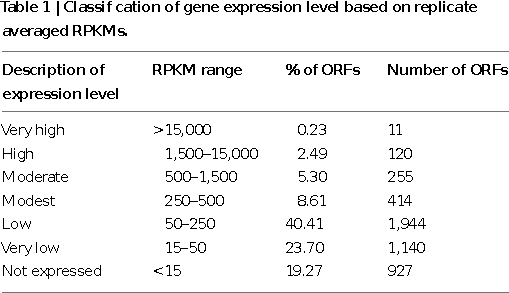
\includegraphics[width=0.7\textwidth]{./tex/chapter1/figures/matsen_OB3b_table1_page--cropped.pdf}
     \begin{singlespace}
     %\caption{}  If you don't put a caption, LaTeX doesn't number that figure.  Woot!
     \label{table:OB3b_1}
     \end{singlespace}
\end{figure}

In order to determine whether the draft genome of the strain is missing some functional genes, we performed de novo assembly of the transcriptome.
Using this approach, a total of 173 genes that are not present in the genome sequence, but have homologs in the non-redundant database were detected.
Among those are key subunits of succinate dehydrogenase (sdhABCD), 2-oxoglutarate dehydrogenase (E2), and nitric oxide reductase (norB) (Table S1 in Supplementary Material).
The de novo transcriptome assembly provides additional information for highly expressed genes and it was used for verification of some metabolic functions that were predicted by enzymatic studies but were not detected in the draft genome assembly (see below).

In addition, the reads obtained from RNA-seq were aligned to the reference genome in order to identify transcription boundaries and transcription start sites for the most highly expressed genes, including the pmoCAB operons, mxaFJGI operon, fae1, pqqA, and key genes of the serine cycle (Table S2 in Supplementary Material, see description below).
Gene expression data were used to reconstruct central metabolic pathways in M. trichosporium OB3b (Table 2; \ref{fig:A_metabolic_map}; Table S2 in Supplementary Material).
Core functions are described below.


\begin{figure}[H]
\centering
     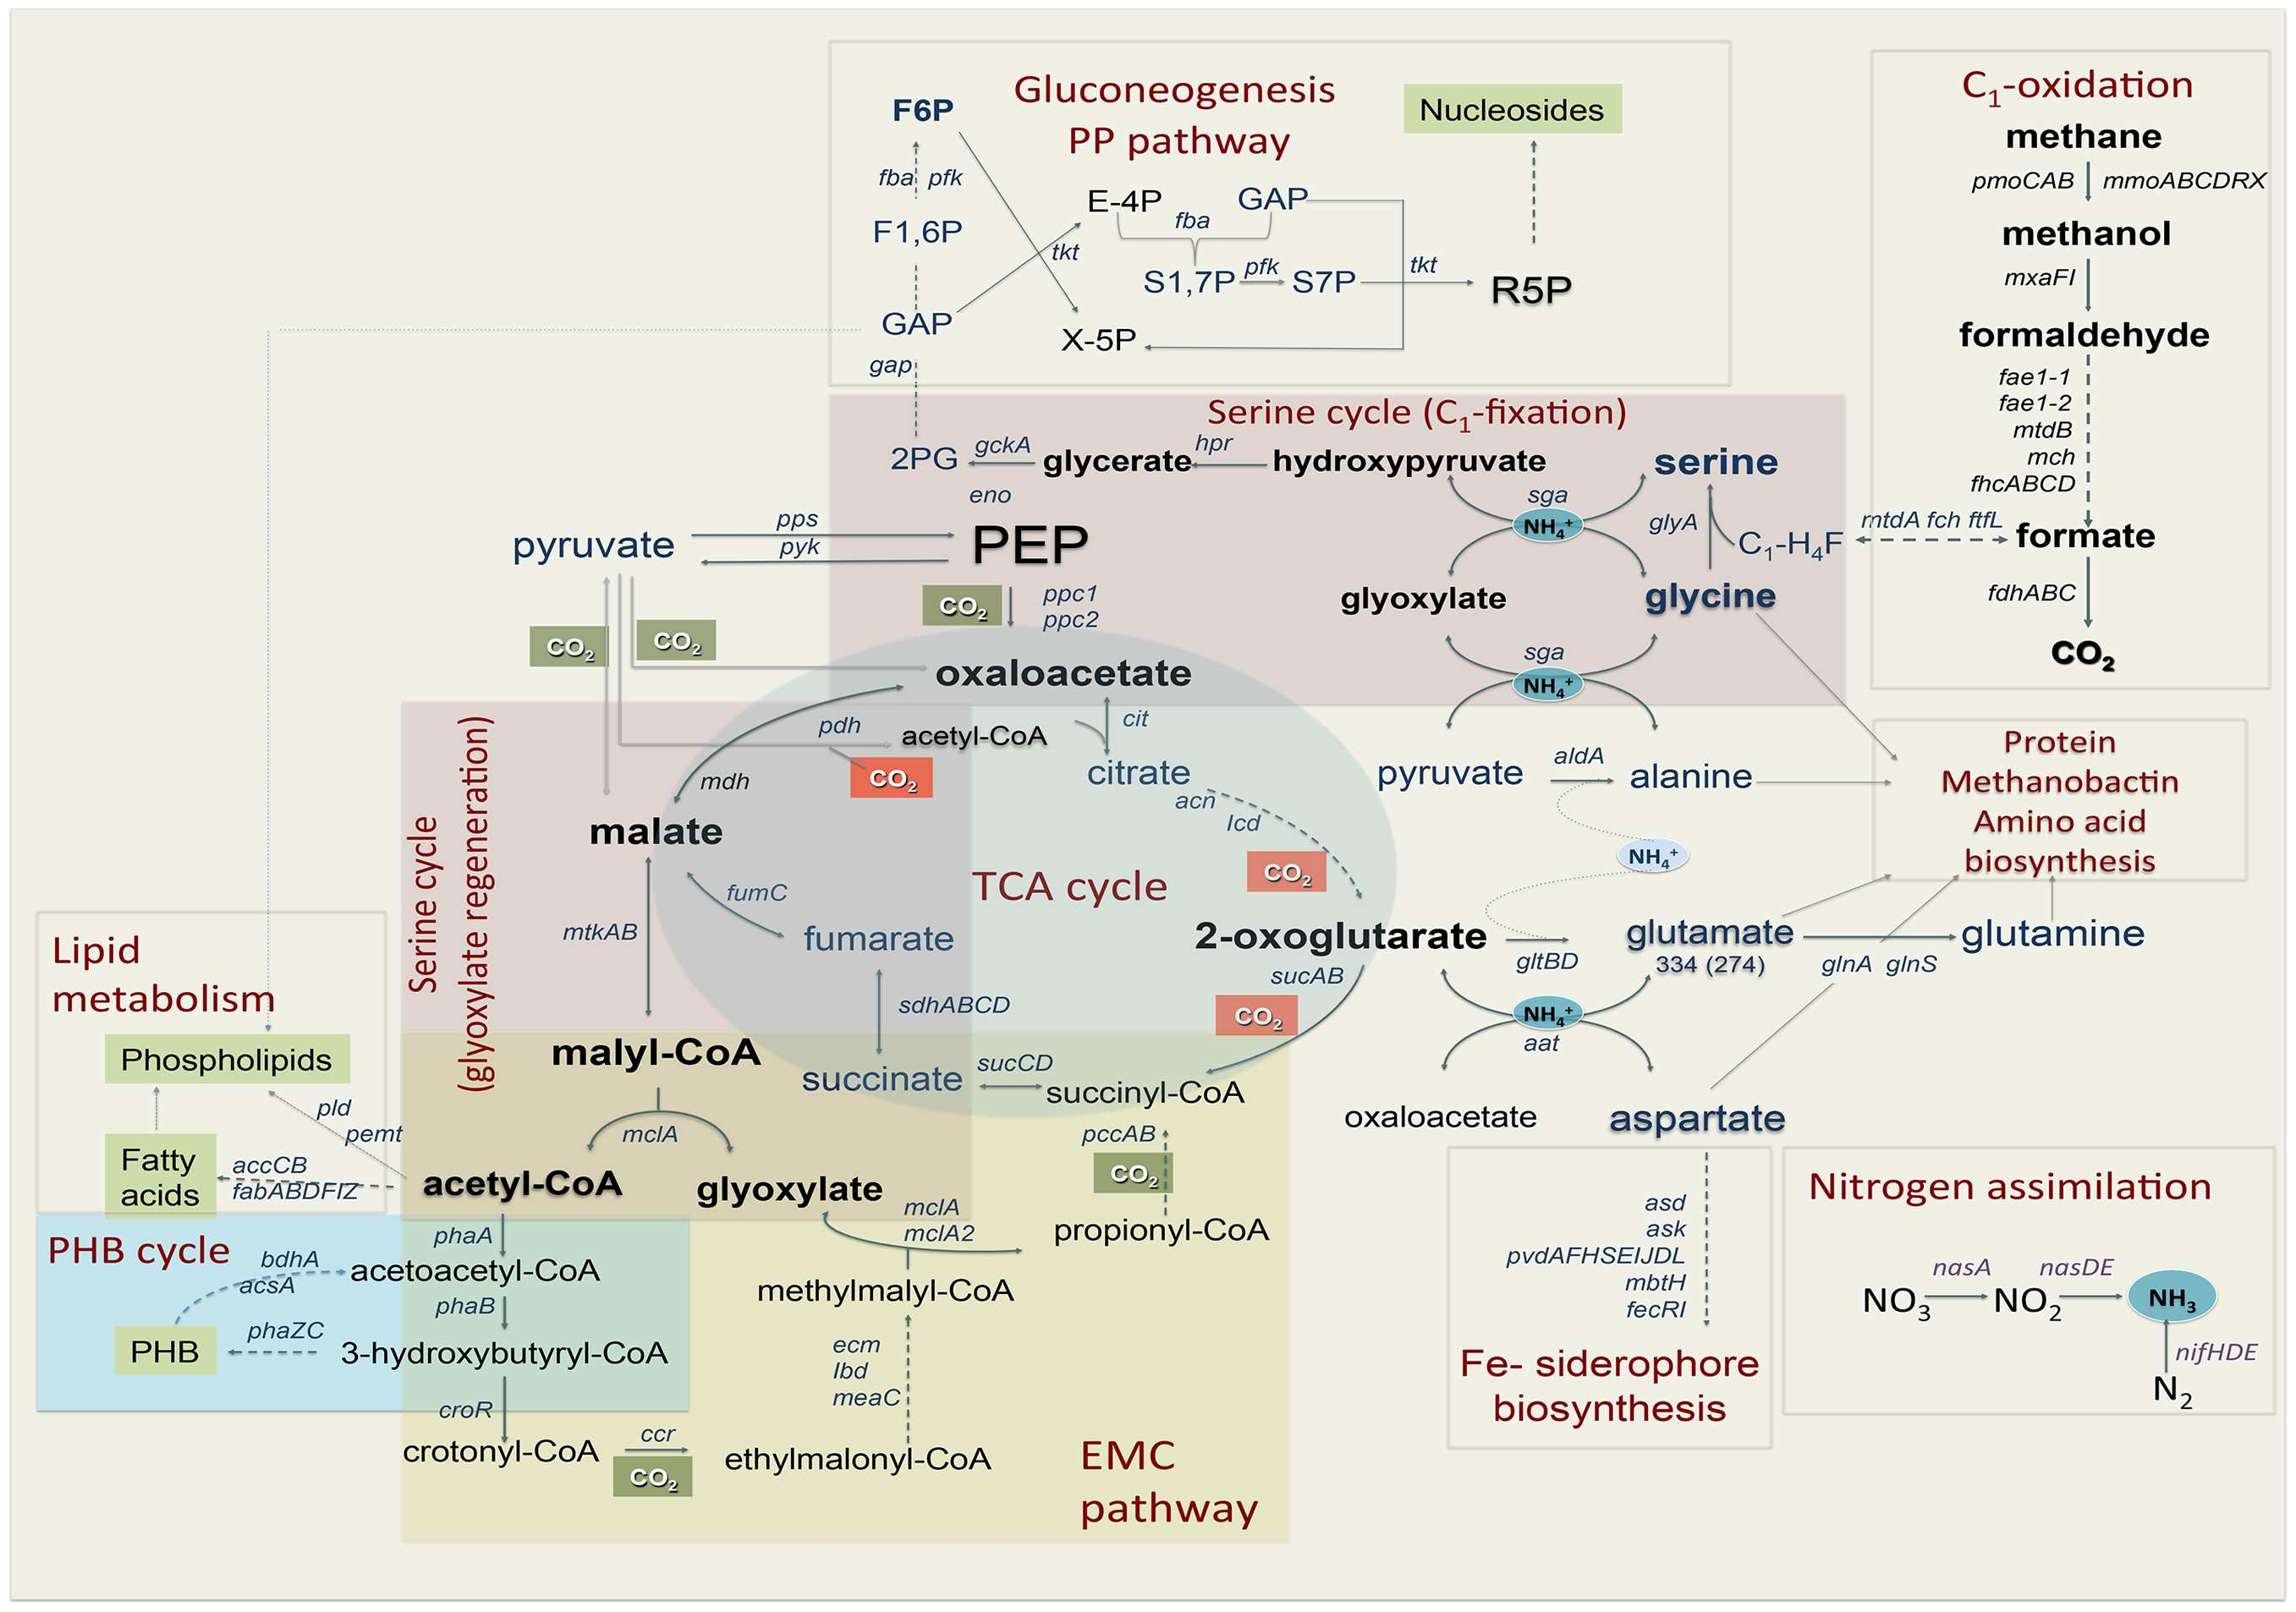
\includegraphics[width=1.0\textwidth]{./tex/chapter1/figures/figure1.png}
     \begin{singlespace}
     \caption[Central metabolism of \textit{Methylosinus trichosporium} OB3b]{
        Central metabolism of \textit{Methylosinus trichosporium} OB3b grown on methane as sole source of energy and carbon as
        deduced from the genome sequences and transcriptomic studies.
        Font size of the gene name indicates the expression level.}
     \label{fig:A_metabolic_map}
     \end{singlespace}
\end{figure}

\begin{figure}[H]
\centering
     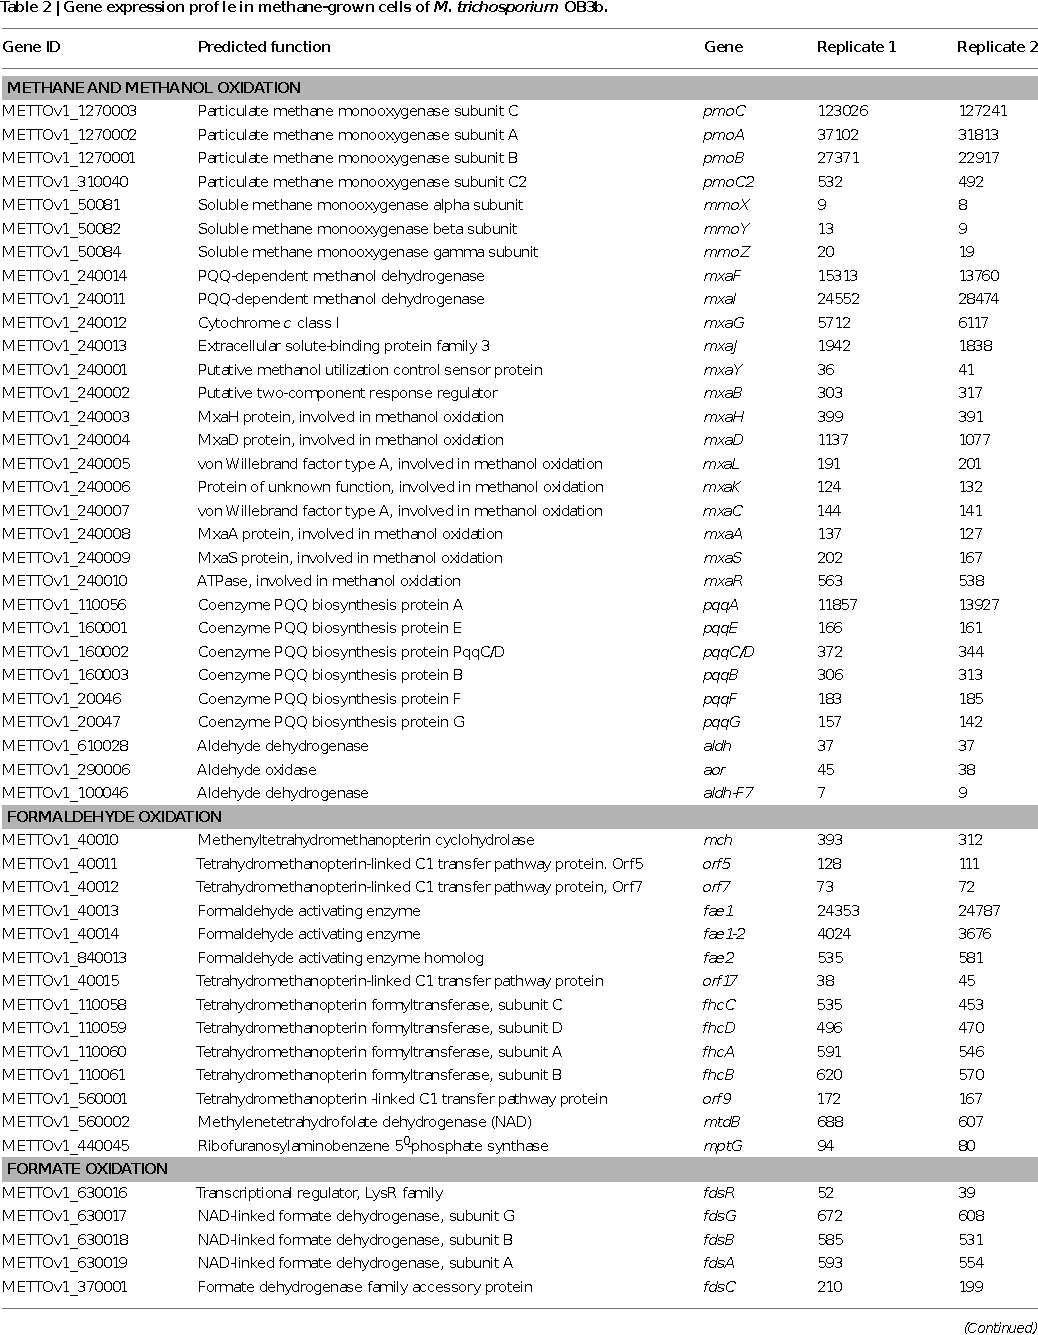
\includegraphics[width=1.0\textwidth]{./tex/chapter1/figures/matsen_OB3b_table2_piece1--cropped.pdf}
\end{figure}

\begin{figure}[H]
\centering
     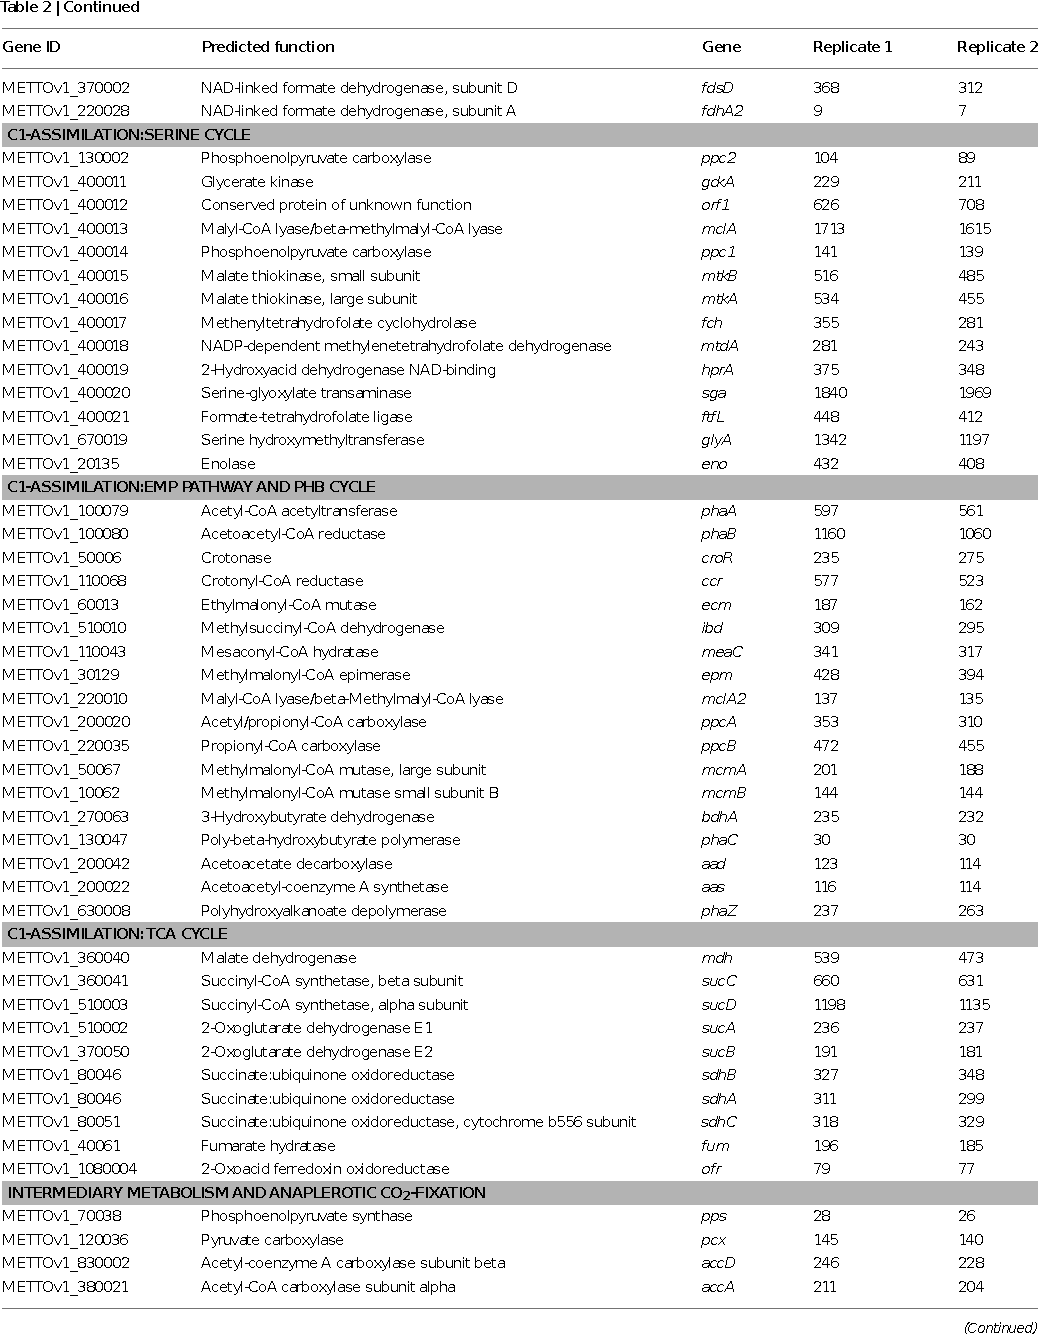
\includegraphics[width=1.0\textwidth]{./tex/chapter1/figures/matsen_OB3b_table2_piece2--cropped.pdf}
\end{figure}

\begin{figure}[H]
\centering
     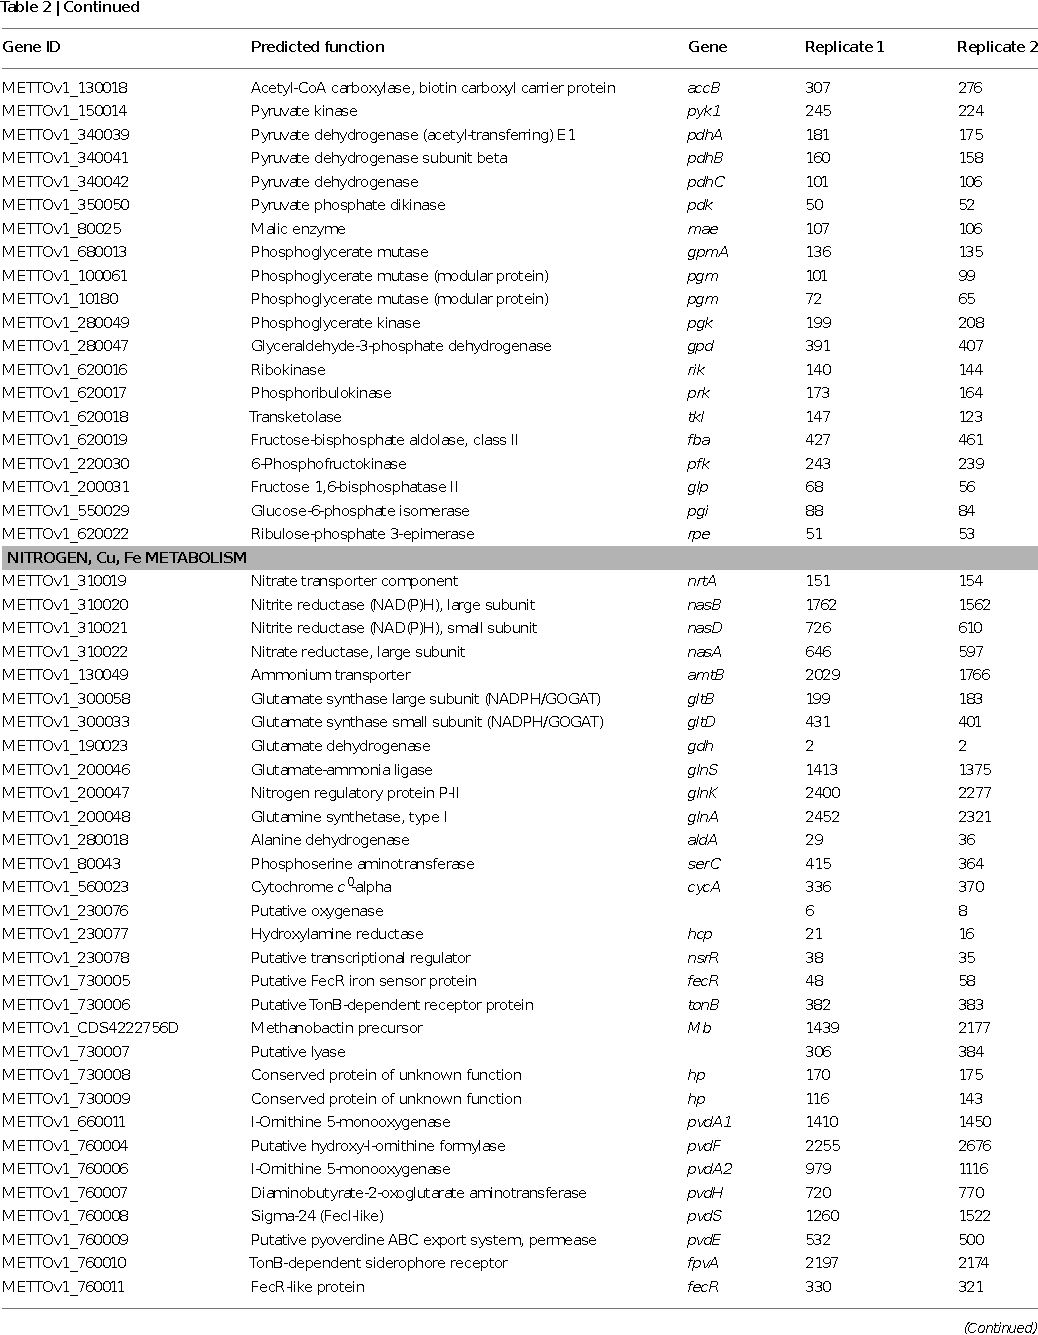
\includegraphics[width=1.0\textwidth]{./tex/chapter1/figures/matsen_OB3b_table2_piece3--cropped.pdf}
\end{figure}

\begin{figure}[H]
\centering
     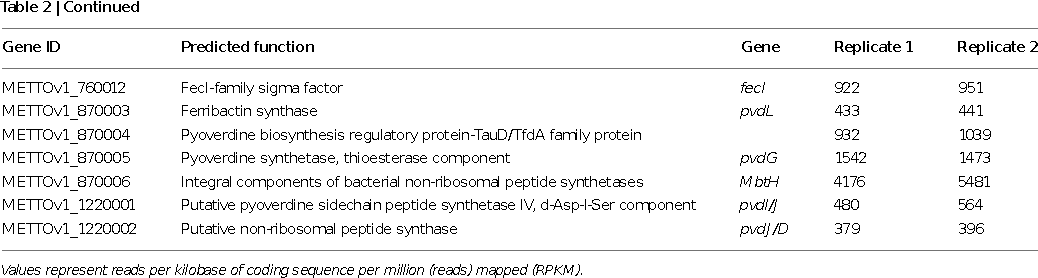
\includegraphics[width=1.0\textwidth]{./tex/chapter1/figures/matsen_OB3b_table2_piece4--cropped.pdf}
\end{figure}


\subsection{\ce{C1}-Oxidation: Methane-To-Methanol}
It has been previously demonstrated that M. trichosporium OB3b possesses two types of methane oxidation enzymes: pMMO and sMMO.
The expression of the enzymes is determined by copper availability; sMMO is dominant in copper-limited environments while pMMO dominates under copper sufficiency \cite{hakemian2007, semrau2010}.
Structures of both enzymes are available \cite{elango1997, hakemian2008}.
In this study, M. trichosporium OB3b was grown at a copper concentration that has been shown to be sufficient to suppress the expression of sMMO \cite{park1991, phelps1992, nielsen1997, lloyd1999, murrell2000}.
Indeed, virtually no expression of the sMMO gene cluster (mmoXYBZC) was observed.
In contrast, the pmoCAB genes were the most highly expressed in the transcriptome, representing about 14\% of all reads mapped to the coding regions (Table 2).
It has previously been shown that PMMO in M. trichosporium OB3b is encoded by two copies of the pmoCAB operon that appear to be identical \cite{gilbert2000}.
The current genome assembly failed to resolve these closely related duplicated regions.
The pmoCAB genes were found within one relatively short contig, which includes 320 bp upstream from pmoC, and about 66 bp downstream from pmoB.
It is possible that in the genome assembly, the pmo contig represents only those parts of the duplicated regions that are highly similar.
Thus, it was not possible to determine relative expression of the two operons with the transcriptomic data.

Previous attempts to identify transcriptional starts of the pmoCAB operons in M. trichosporium OB3b using a conventional primer extension approach were not successful \cite{gilbert2000}.
The RNA-seq data were used for identification of transcriptional starts for the pmoCAB operons.
Because the published METTOv1 genome did not contain a complete pmoCAB cluster, a separate alignment run was performed using a previously published sequence as the scaffold \cite{holmes1995}.
For this sequence, two possible transcriptional start sites were identified.
It is not known whether these reflect the same start sites of both operons, different start sites for each, or expression of only one operon with two start sites.
The position -274nt (A) from the translational start of the pmoC gene was predicted as the most prominent start of transcription of the operon (Figure \ref{fig:S1} in Supplementary Material).
Putative $\sigma_{70}$-like -10 and -35 regions could be identified upstream of the predicted start (Table S3 in Supplementary Material).
The structure of the putative promoter region from M. trichosporium OB3b shows significant similarity to a pmoCAB promoter region previously identified in Methylocystis sp. M \cite{gilbert2000}.
Another potential transcriptional start is at position -324 from the translational start of the pmoC gene.
It should be noted that the region between the two predicted start sites was also covered with relatively high count (region between -324 and -274nt with respect to the translational start of pmoC).
No putative promoter sequences were found upstream of position 324.

The genome predicts an additional copy of the pmoC gene by itself (pmoC2, METTOv1\_310040), which can be distinguished from the other pmoC genes in the transcriptomics data due to sequence divergence.
It has previously been demonstrated that additional copies of pmoC are essential for methanotrophic growth in other strains \cite{stolyar1999, dam2012a}.
It has also been shown that the homologous amoC (additional lone copy of amoC in ammonia-oxidizing bacterium Nitrosomonas europaea) plays role in cell recovery from ammonium starvation \cite{berube2012}.
However the functional role of PmoC is not known.
The relative expression of pmoC2 was approximately 450-fold less than the expression of the two pmoC genes from the pmo-operons (Table 2).
Low relative expression of the pmoC homolog may suggest a role in regulation or sensing rather than catalytic activity.

\subsection{\ce{C1}-Oxidation: Methanol-To-Formaldehyde}
The product of methane oxidation (i.e., methanol) is converted to formaldehyde by a PQQ-dependent methanol dehydrogenase (MDH) \cite{anthony1982, anthony2002, yamada1992, anthony1994}. % Yamada really is 1992.
The enzyme has been previously purified from M. trichosporium OB3b and well characterized \cite{yamada1992}.  % Yamada really is 1992.
MDH is a hetero-tetrameric enzyme encoded by mxaF and mxaI.
The activity of the enzyme in vivo requires cytochrome cL (mxaG) and a number of chaperones, regulators, and enzymes, including genes required for \ce{Ca^{2+}} insertion \cite{anthony1994, anthony2002}.
Most of the genes essential for this methanol conversion step in M. trichosporium OB3b are organized in one large operon in an order similar to that found in other methylotrophs (Figure \ref{fig:S2}A in Supplementary Material).
The first four genes of the operon (mxaFJGI), encoding the two subunits of the MDH, the associated cytochrome, and a gene of unknown function (mxaJ) were detected at relatively high RPKM counts.
The relative expression of genes downstream from mxaI, including those for chaperones, regulators, and \ce{Ca^{2+}} insertion functions drops by 10- to 50-fold (Table 2).
The overall mapping pattern of the mxa-cluster is as follows: mxaFJGI (highly expressed), mxaD (moderate expression), mxaRSACKL, mxaB (low expression), and mxaY (very low expression).
It remains to be elucidated if the mxaRSACKL transcripts arise from the same start as mxaF and are attenuated by some transcriptional or post-transcriptional mechanism, or whether separate, lower expression promoter(s) is/are present.
Orientations and/or the expression patterns of mxaD, mxaB, and mxaY, suggest that they are not part of the major mxaF-operon (Figure \ref{fig:S2}A in Supplementary Material) and most likely have independent regulatory/promoter regions.
According to RNA-seq mapping data, a putative transcriptional start of the mxaFJGI operon is predicted at position -164 from the predicted translational start (Figure \ref{fig:S3} in Supplementary Material).
Just upstream from the predicted transcriptional start, putative $\sigma^{70}$-like -10 and -35 sequences were identified (Table S3 in Supplementary Material).

The genome of M. trichosporium OB3b contains the following three homologs of the large subunit of the MDH: xoxF1, xoxF2, and xoxF3.
Relative expression of all xoxF-homologs is very low.
The most highly expressed xox-homolog (xoxF1) showed only about 2\% of the mxaF expression.
The function of the xox-gene products has not been studied in M. trichosporium OB3b.
In the non-methanotrophic methylotroph Methylobacterium extorquens AM1, it has been shown that xoxF may display methanol-oxidizing activity \cite{schmidt2010}, and can contribute to the complex regulation of mxa-genes \cite{skovran2011}.
Furthermore, there are suggestions that xoxF may play a role in formaldehyde oxidation \cite{wilson2008}.
The low expression of all xoxF-homologs in M. trichosporium OB3b compared to mxaFI or \ce{H4}MTP-linked pathway genes suggests that xox-genes may have no or a minor contribution to methanol oxidation in M. trichosporium OB3b under the tested growth conditions.
However, our data do not rule out the possibility that one or more of the xoxF gene products are involved in regulation, either of methanol or formaldehyde oxidation.

Pyrroloquinoline quinone (PQQ) biosynthesis is another function essential for operation of the primary methanol oxidation system \cite{toyama1997, anthony2002}.
A total of six pqq genes appear to be present in the M. trichosporium OB3b genome in two clusters: pqqBCDE and pqqFG.
Moderate expression of both clusters was observed (Table 2).
No gene for the small PQQ precursor (PqqA) is predicted in the current version of the genome.
Our manual review of the sequences revealed a fragment within the METTOv1\_110055 – METTOv1\_110057 gene locus (positions 1424678 – 1424755 of current version of the genome) with high sequence identity [83\% nucleic acid (NA) identity and 96\% amino acid (AA) similarity] to the pqqA sequence from Methylobacterium spp (Figures 2A,B).
Transcript mapping data indicated that only the pqqA-like region of the locus is highly expressed (\ref{fig:B_pqqA}C).
The relative expression of the putative PQQ precursor gene is comparable to the high expression of the mxaFI genes.
The rest of the genes involved in PQQ biosynthesis showed modest to low expression (Figure \ref{fig:S2}B in Supplementary Material).

\begin{figure}[H]
\centering
     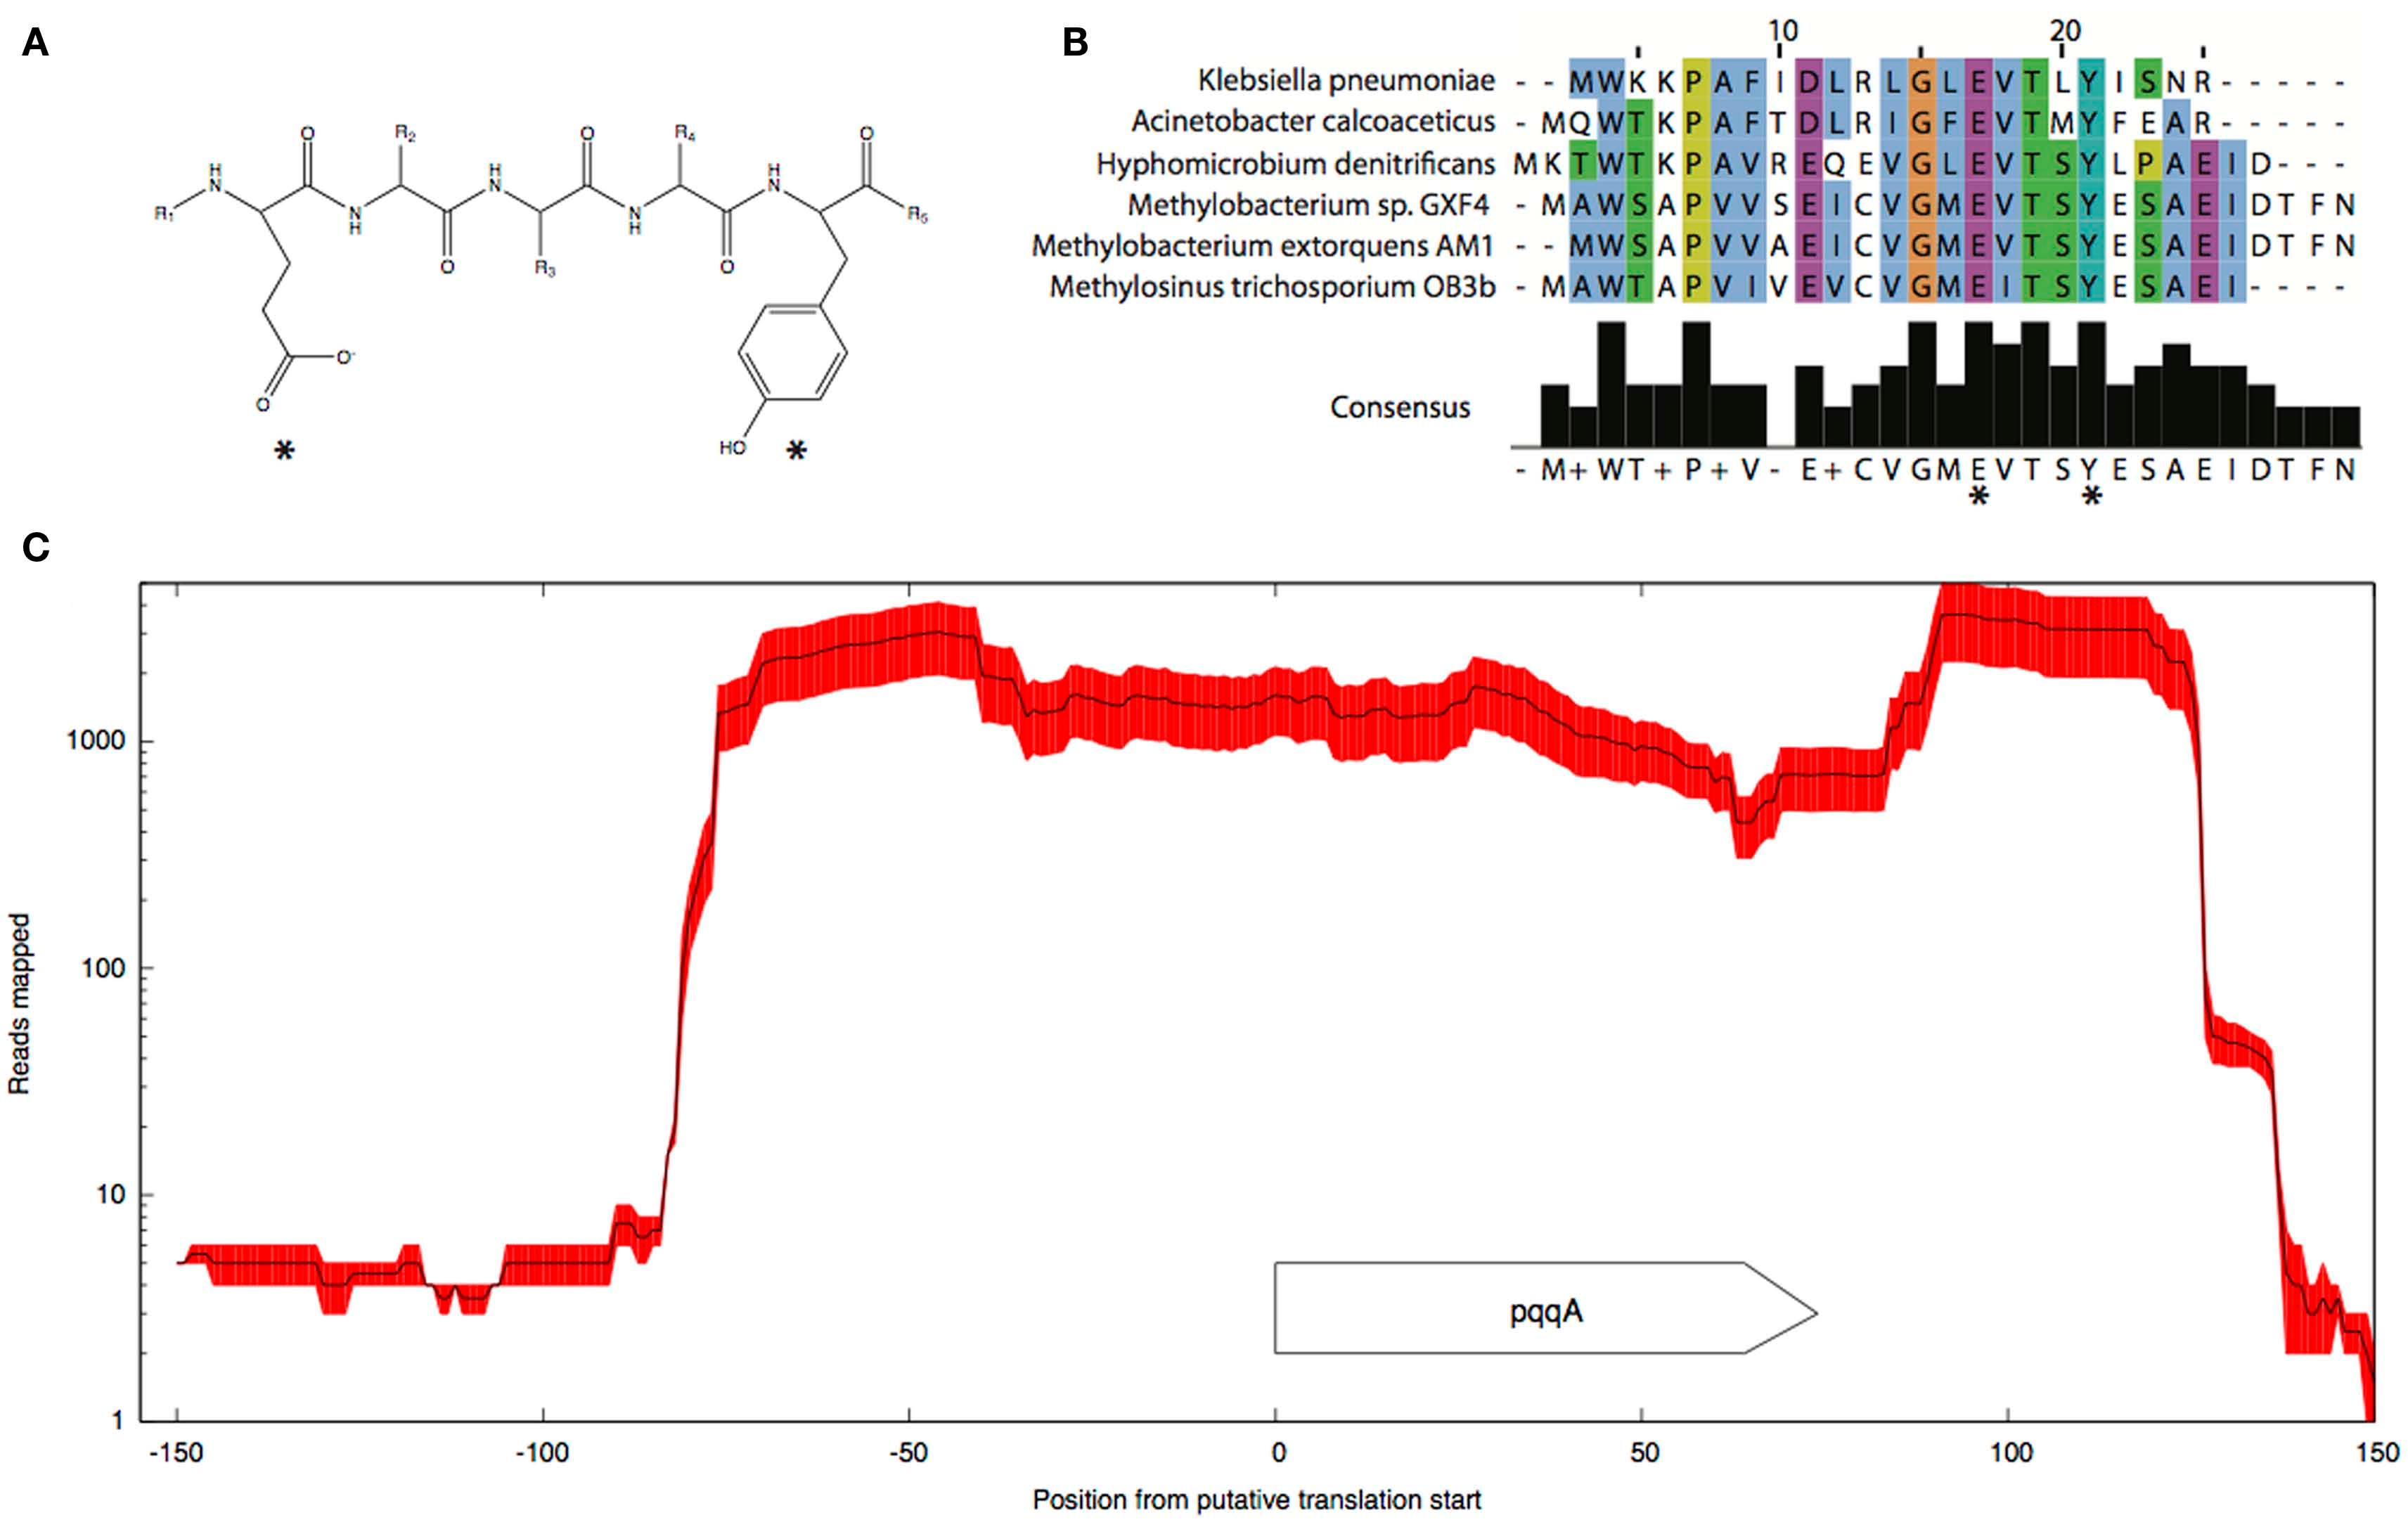
\includegraphics[width=1.0\textwidth]{./tex/chapter1/figures/figure2.png}
     \begin{singlespace}
     \caption[pqqA structure, alignment, and RNA-seq coverage]{
        Predicted structure
        (A) and alignment of the putative pqqA peptide
        (B) from M. trichosporium OB3b and pqqA peptides from Methylobacterium sp. GXF4, M. extorquens AM1,
            Hyphomicrobium denitrificans ATCC51888, K. pneumoniae, and A. calcoaceticus.
        (C) Mapping.}
     \end{singlespace}
     \label{fig:B_pqqA}
\end{figure}


\subsection{\ce{C1}-Oxidation: Formaldehyde-To-Formate}
Previous enzymatic studies predict three possible pathways for formaldehyde oxidation: (1) direct oxidation through dye-linked heme-containing formaldehyde dehydrogenase \cite{patel1980}, (2) \ce{H4}folate-, and (3) \ce{H4}MTP-mediated \ce{C1} transfers \cite{vorholt1999, doronina2008}.
Contrary to enzymatic studies, BLAST searches of the draft genome of M. trichosporium OB3b did not reveal any obvious system that could be attributed to heme-containing formaldehyde oxidation.
Three broad-specificity aldehyde-detoxification systems, including two NAD-dependent aldehyde dehydrogenases (Aldh-F7 METTOv1\_100046 and Aldh, METTOv1\_610028) and one aldehyde oxidase (Aor, METTOv1\_290006) were predicted in the genome.
Two of them, aldh and aor show low expression (Table 2), while aldh-F7 was barely detected in the transcriptome.
None of the putative genes identified by de novo transcriptome assembly could be readily attributed to any dye-linked aldehyde dehydrogenases (Schwartz et al., 2004).
Thus, even if the enzyme is present in the genome, its expression during growth of the strain on methane must be low.

For years it has been assumed that methylene \ce{H4F} is formed as a result of the spontaneous (non-enzymatic) condensation of formaldehyde with \ce{H4F} (Large and Quayle, 1963).
It has recently been demonstrated that formate, rather than formaldehyde serves as an entry substrate for assimilation in serine cycle methylotrophs (Crowther et al., 2008).
With this metabolic arrangement, the \ce{H4}Folate \ce{C1} transfer could be considered as a part of the assimilatory network that converts formate into methylene \ce{H4}F.
In M. trichosporium OB3b genes encoding all three steps of the \ce{H4}Folate pathway converting methylene-\ce{H4}F to formate (formyl-\ce{H4}F ligase, ftfL, methenyl-\ce{H4}F cyclohydrolase, fch, and methylene-\ce{H4}F dehydrogenase mtdA) were co-localized and co-transcribed with genes encoding the serine cycle enzymes (Figure \ref{fig:S4} in Supplementary Material).
While the assimilatory function of the pathway is more apparent, it is still possible that key enzymes of the pathway contribute to formaldehyde oxidation in M. trichosporium OB3b.

The tetrahydromethanopterin (\ce{H4}MTP) pathway was proposed to be the key pathway for formaldehyde oxidation/detoxification in alphaproteobacterial methylotrophs (Chistoserdova et al., 1998).
It was speculated that this pathway contributes to formaldehyde oxidation in methane utilizing proteobacteria (Vorholt et al., 1999).
Nineteen genes encoding enzymes and genes for tetrahydromethanopterin biosynthesis were identified in the M. trichosporium OB3b genome.
These genes were not clustered together in the genome, but formed five different gene islands: (1) mch-orf5-orf7-fae1/1-fae1/2-orf17 (Figure \ref{fig:S2}C in Supplementary Material); (2) orf19-orf20-afpA-orf21-orf22; (3) fhcCDAB; (4) orf9-mtdB; and (5) pcbD-mptG.
No homologs of orfY, dmrA, and pabB genes, which are commonly associated with tetrahydromethanopterin biosynthesis in methylotrophs (Caccamo et al., 2004; Rasche et al., 2004; Chistoserdova et al., 2005; Kalyuzhnaya et al., 2005), were found in the genome or detected in transcriptome.

Formaldehyde activating enzyme (FAE) is the first enzyme of the \ce{H4}MTP-pathway, which has been shown to catalyze the condensation of formaldehyde and \ce{H4}MPT to form methylene-\ce{H4}MPT (Vorholt et al., 2000).
The draft genome of M. trichosporium OB3b predicts three homologs of Fae; two of them (fae1/1 and fae1/2) share a high degree of identity (NA 82.2\%) and are co-localized in the genome (Figure \ref{fig:S2}C in Supplementary Material).
Though both fae genes are clustered with four other genes involved in the \ce{H4}MTP-pathway, they are expressed in dramatically different patterns.
The abundance of fae1-1 transcripts was almost 40-fold higher than the abundance of any other gene in the cluster, except fae1-2 (Table 2; Figure \ref{fig:S2}C in Supplementary Material).
The relative abundance of the second homolog (fae1-2) was one fifth of that observed for fae1-1, and fae1-2 was the second highest expressed gene in the pathway.
Mapping data indicate that fae1-1 and fae1-2 are most likely co-transcribed (Figure \ref{fig:S5} in Supplementary Material).
RNA-Seq mapping data suggest two putative transcriptional starts at the positions -215 (with $\sigma^{70}$-like -10 and -35 sequences upstream) and –105 (with a conserved “AATGGTTG” sequence in the -35 region) upstream from the fae1-1 translational start (Figure \ref{fig:S5} in Supplementary Material; Table S3 in Supplementary Material).

The third homolog of Fae (fae2) demonstrates moderate expression.
The rest of the genes encoding key enzymes of the pathway (mtdB, methylene-\ce{H4}MPT dehydrogenase; mch, methenyl-\ce{H4}MPT cyclohydrolase; fhcABCD, formyltransferase/hydrolase) have a similarly moderate expression.
The relative abundance of genes encoding key enzymes of the pathway were 5- to 10-fold higher than those involved in cofactor biosynthesis.
Overall, transcriptomic data indicate that the \ce{H4}MTP-pathway serves as the key pathway for formaldehyde oxidation in M. trichosporium OB3b.

\subsection{Formate Oxidation}
Formate is oxidized to \ce{CO2} by a NAD-dependent formate dehydrogenase in most, if not all, methanotrophs \cite{anthony1982}.
It has been suggested that most of the reducing power required for methane metabolism is produced by formaldehyde oxidation to formate and then to \ce{CO2} \cite{hanson1996}.
It has been speculated that in microbes with a functional serine pathway, formate serves as a key branch point between assimilation and catabolism (Chistoserdova, 2011).
NAD-dependent formate dehydrogenase from M. trichosporium OB3b has been purified and characterized (Jollie and Lipscomb, 1991).
The enzyme is composed of four subunit types and contained flavin, iron, and molybdenum (Jollie and Lipscomb, 1991).
The genome of M. trichosporium OB3b predicts one NAD-dependent molybdenum-containing formate dehydrogenase encoded by fdsABGCD and an additional single copy of the alpha subunit (fdhA).
The two genes fdsA and fdhA share 81\% identity.
Only one of them, fdsA as well as the rest of the fds cluster genes were expressed in the transcriptome (Table 2).

\subsection{\ce{C1}-Assimilation: Serine Cycle}
It has been previously suggested that the serine cycle is the major pathway for \ce{C1}-assimilation in M. trichosporium OB3b \cite{strom1974}.
All genetic elements essential for operation of the cycle were predicted in the genome and cluster together \cite{stein2010}.
However, genes of the pathway show deferent levels of expression (Table 2).
While sga, glyA, and mclA have high expression levels, the rest of the genes involved in the pathway show modest expression (Table 2; Figure \ref{fig:S4} in Supplementary Material).
In addition to the serine-glyoxylate aminotransferase (sga), a key aminotransferase in the central metabolism of serine cycle microbes, moderate levels of expression were observed for two other aminotransferases, phosphoserine aminotransferase, and aspartate aminotransferase (Table 2).

The genome of M. trichosporium OB3b encodes two copies of phosphoenolpyruvate (PEP) carboxylase (ppc1 and ppc2).
The two enzymes are only distantly related to each other and share 33\% identity at the amino acid level.
One of them, Ppc1, clusters with PEP carboxylases usually found in bacteria possessing the serine cycle for \ce{C1}-assimilation (\ref{fig:C_pep}).
Serine cycle Ppcs belong to a “non-regulated” group of PEP carboxylases \cite{anthony1982}.
The activity of these enzymes is not controlled by intermediates of the TCA cycle or glycolysis/gluconeogenesis (Newaz and Hersh, 1975).
The second homolog of Ppc (ppc2) clusters with anaplerotic “regulated” PEP carboxylases, which are controlled by a variety of metabolic effectors (Takahashi et al., 1993; Kai et al., 2003).
Both ppc1 and ppc2 transcripts demonstrate comparable levels of abundance in this study (Table 2).
The sequences of the two genes were further investigated in an attempt to better understand the rationale for the enzymatic redundancy at the PEP to oxaloacetate conversion step.
We used multiple sequence alignments of Ppc1, Ppc2, and other characterized PEP carboxylases and homology models (not shown) built from tensed and relaxed state crystal structures (Matsumura et al., 2002) to investigate the predicted allosteric regulation sites of these two enzymes.
The alignment shows that only the catalytic elements, such as PEP-binding-site residues, are conserved in both proteins (Ppc1 and Ppc2). %, Figure S6 in Supplementary Material).
However, sequence features required for the allosteric regulation of the enzyme activity show several structural differences.
The majority of the characterized bacterial PEP carboxylases are activated by acetyl-CoA, FBP, long-chain fatty acids, and pGp.
Inhibition occurs in the presence of aspartate and L-malate.
In the case of Ppc1 from M. trichosporium OB3b, two of the four highly conserved polar amino acids that bind allosteric inhibitors (e.g., aspartate, malate) were hydrophobic: L805 and A912 (K and N in E. coli respectively) suggesting alternate inhibitors or a lack of sensitivity to L-malate and aspartate.
The activator-binding residues were conserved except for a R159 instead of K.
By contrast, Ppc2 was well conserved relative to the well characterized PEP carboxylases and for those with structures, only minor rearrangements of the monomeric interfaces were predicted.
It is tempting to speculate that the presence of two functionally identical but differently regulated enzymatic systems in M. trichosporium OB3b evolved as a way to control flux through PEP-oxaloacetate in response to levels of the serine cycle and EMC pathway intermediates.
The flux is never completely blocked, due to the insensitivity of Ppc1 to the metabolic state of the cell.
Increases in the intracellular levels of acetyl-CoA, aspartate, or malate (as a result of saturation of the downstream EMC pathway and the TCA cycle) can reduce the flux through the PEP-oxaloacetate presumably twofold via allosteric inhibition and lack of activation of Ppc2 activity.
In this case, \ce{C1}-carbon assimilated via the serine cycle is re-directed to gluconeogenesis or converted into pyruvate.

\begin{figure}[H]
\centering
     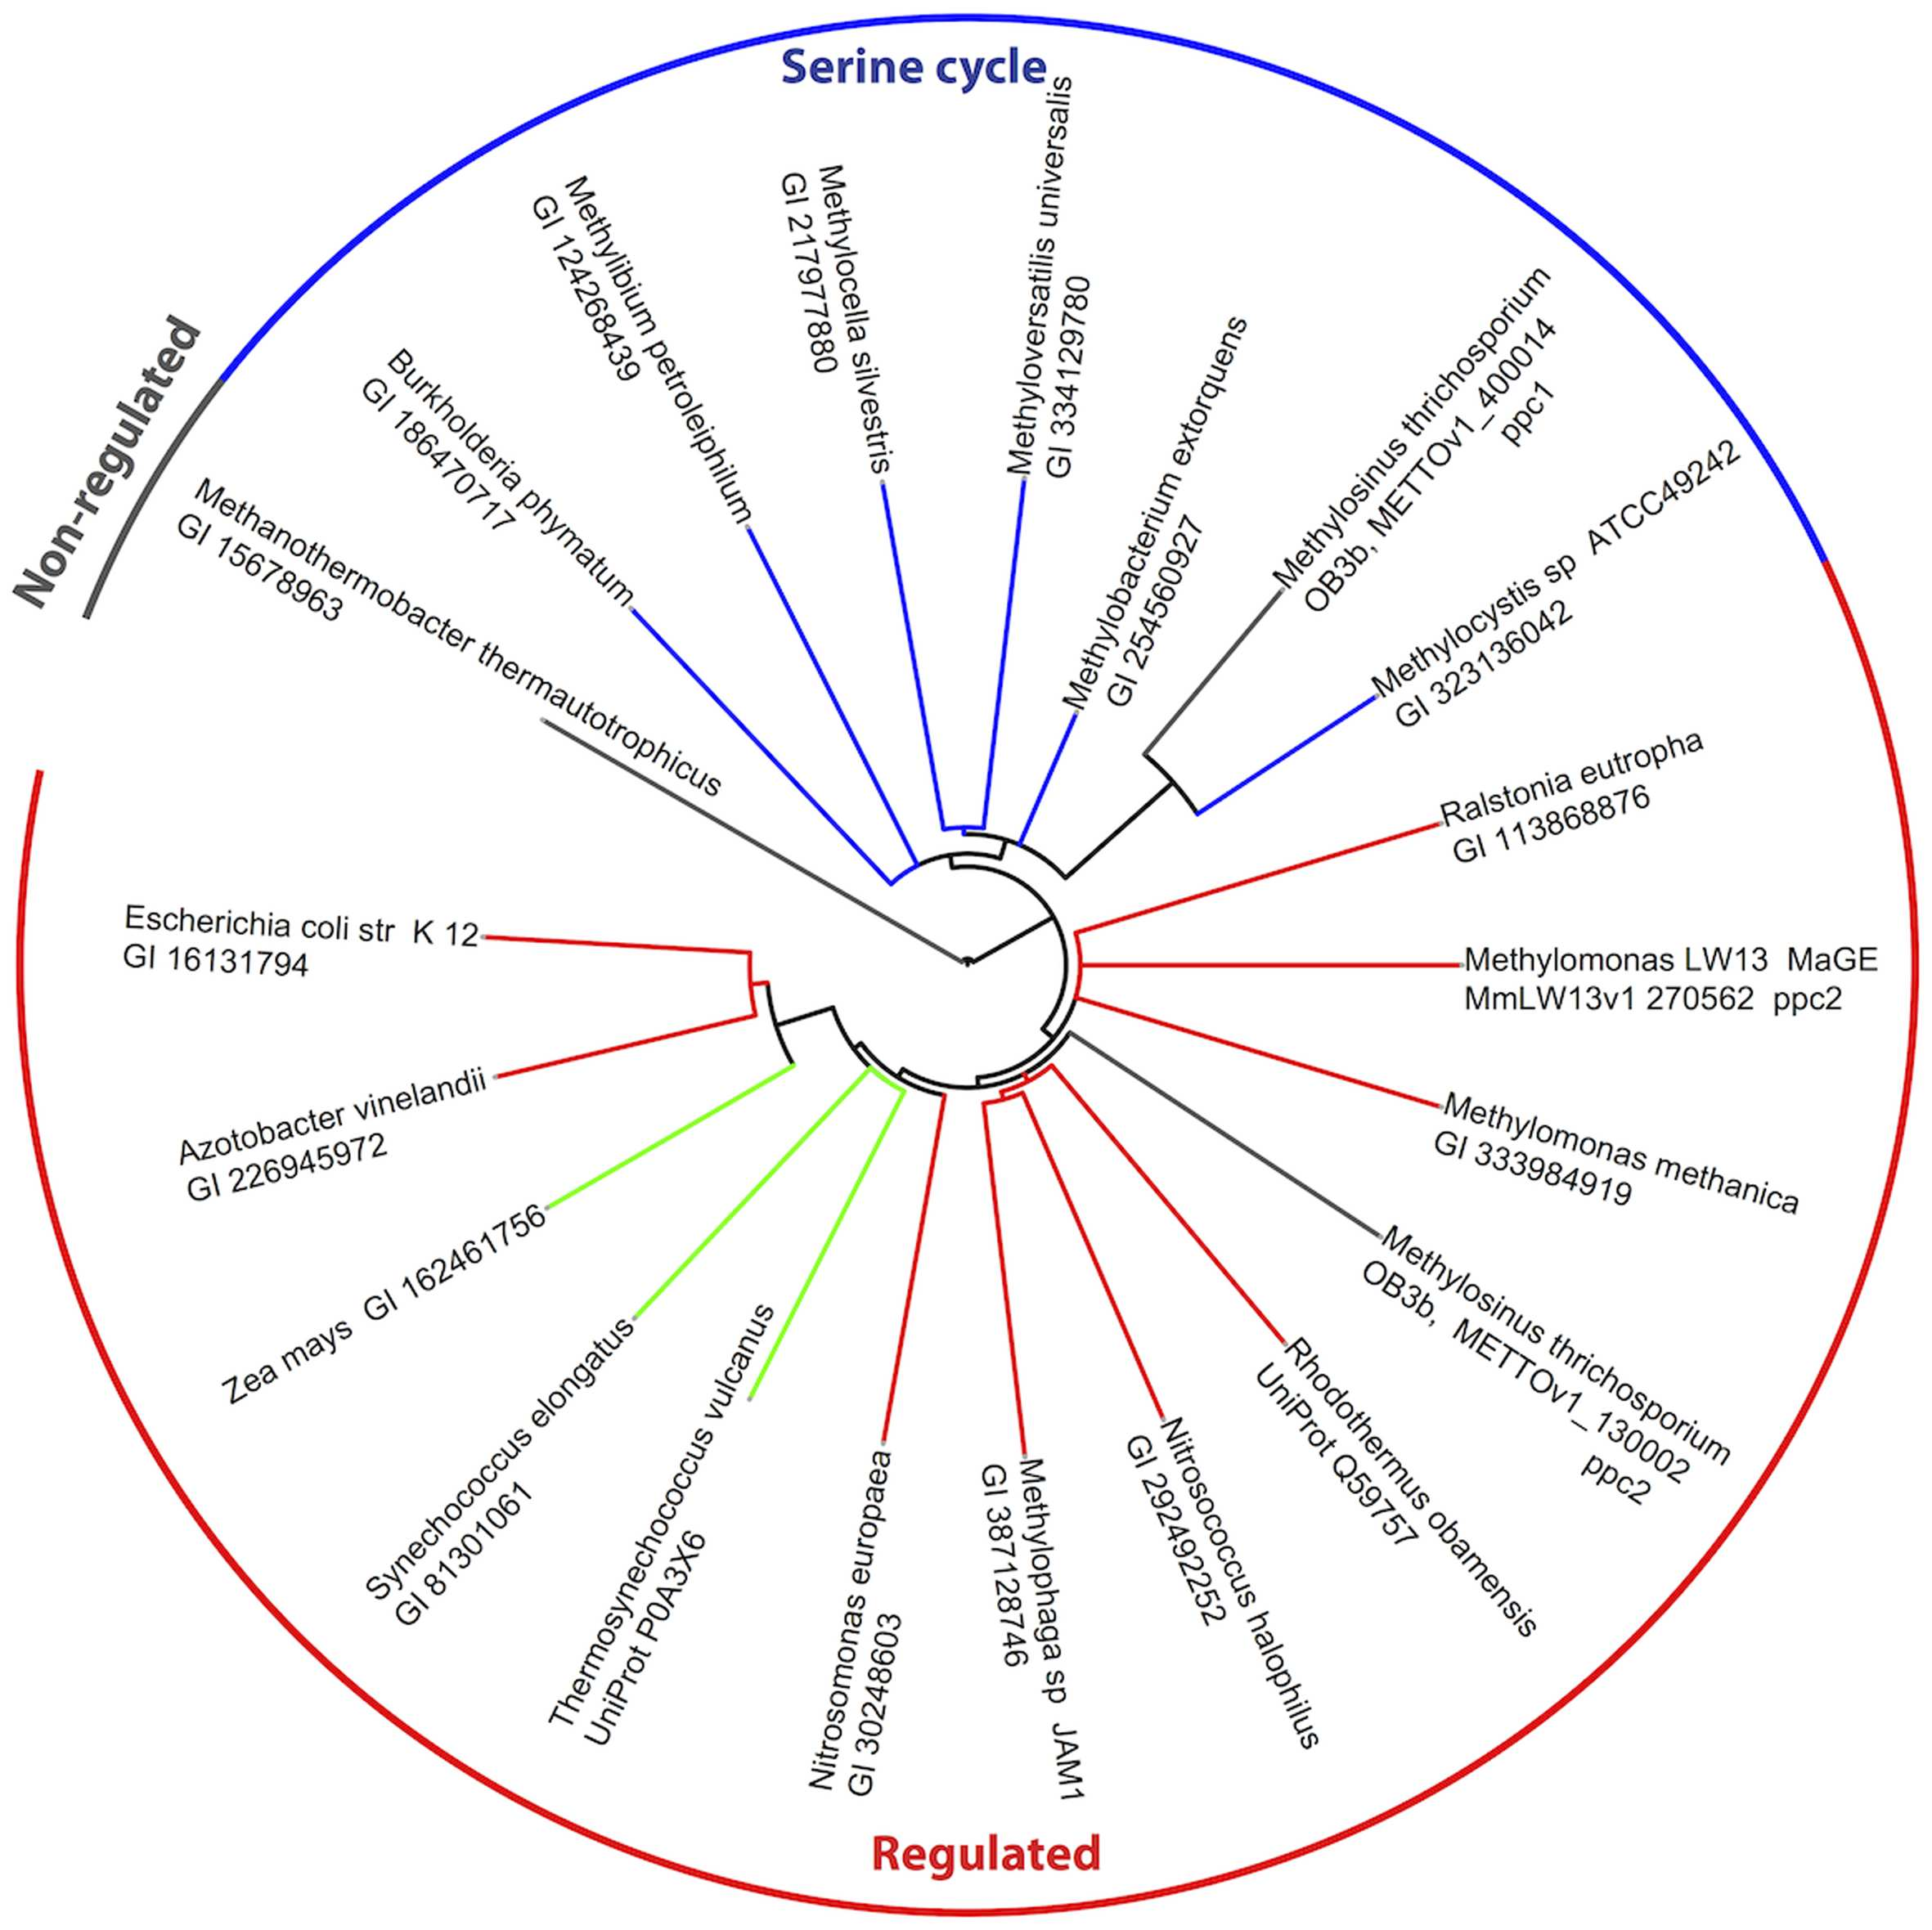
\includegraphics[width=1.0\textwidth]{./tex/chapter1/figures/figure3.png}
     \begin{singlespace}
     \caption[Phylogenetic tree of phosphoenolpyruvate carboxylases.]{
        Phylogenetic tree of phosphoenolpyruvate carboxylases.
        Sequence identifiers follow the source organism label. Sequences were aligned with MUSCLE v3.8.31 (Edgar, 2004) and
        the tree created with ClustalW2 2.0.12 (Larkin et al., 2007) and rendered with iTOL (Letunic and Bork, 2007).}
     \end{singlespace}
     \label{fig:B_pep}
\end{figure}

Regeneration of glyoxylate is an essential part of the serine cycle \cite{anthony1982, anthony2011, peyraud2009}.
Like other obligate methanotrophic bacteria, M. trichosporium OB3b lacks isocitrate lyase, a key enzyme of the glyoxylate shunt \cite{trotsenko2008}.
Homologs of enzymes involved in the ethylmalonyl-CoA (EMC) pathway, an alternative route for glyoxylate regeneration \cite{peyraud2009}, were identified in the draft genomes of M. trichosporium OB3b and another obligate methanotroph Methylocystis sp. \cite{stein2010, stein2011}.
However, a functional EMC pathway has not yet been demonstrated in methanotrophs.
Furthermore, the recent investigation of PHB-metabolism in Methylocysctis parvus OBBP, an alphaproteobacterial methanotroph, suggested that this metabolic module can not supply C2 (glyoxylate) units for biosynthesis \cite{pieja2011}.
As the initial steps of the EMC pathway are shared with PHB biosynthesis [acetyl-CoA acetyltransferase (phaA) and acetoacetyl-CoA reductase (phaB), see \ref{fig:A_metabolic_map}] in context with the data presented by Pieja et al. (\cite{pieja2011}) call into question the operation of the EMC pathway in methanotrophs.

We found that genes encoding the initial steps of the PHB-synthesis (phaA/phaB) show moderate levels of expression.
As could be expected for cells in early-mid exponential growth, the expression of the gene encoding PHB synthase (phaC) was low.
The data are consistent with previous observations of high activity of PhaA and PhaB and low activity of PHB synthase (PhaC) in exponentially grown cells of M. trichosporium OB3b \cite{williams1998, doronina2008}.
The PHB-degradation pathway genes, including 3-hydroxybutyrate dehydrogenase, acetoacetate decarboxylase, and acetoacetyl-coenzymeA synthetase, show modest expression levels (Table 2).

All homologs of the EMC pathway enzymes were expressed in M. trichosporium OB3b during growth on methane (Table 2).
Several putative acetyl/propionyl-CoA carboxylases are predicted in the genome, however only METTOv1\_200020 (putative ppcA) and METTOv1\_220035 (putative ppcB) were expressed.
Furthermore, the PpcAB and crotonyl-CoA reductase (ccr) genes display the highest level of expression among all \ce{CO2}-fixing enzymes in the M. trichosporium OB3b transcriptome.
Thus, the transcriptional profile of M. trichosporium OB3b indicates the methanotroph may possess an active EMC pathway.

\subsection{\ce{C1}-Assimilation: TCA Cycle and Anaplerotic \ce{CO2}-Fixation}
All previous enzymatic studies predict that the tricarboxylic acid cycle (TCA cycle) in alphaproteobacterial methanotrophs is complete \cite{trotsenko2008}.
However, the functional role of this metabolic pathway in methanotrophs is not fully understood.
It has been suggested that the main role of the TCA cycle in the methanotrophs is carbon assimilation rather than energy production, due to low enzyme activity and lack of pyruvate dehydrogenase \cite{trotsenko1976, anthony1982, shishkina1982, trotsenko2008}.
However, labeling studies on acetate and pyruvate utilization have predicted the presence of a catabolic TCA cycle in type II methanotrophs \cite{wadzinski1975, higgins1981}.
In silico genome analysis indicates that M. trichosporium OB3b contains predicted genes for all key enzymes of the TCA cycle and pyruvate dehydrogenase (pdh).
All of these genes were expressed (Table 2).
These steps of the TCA cycle are shared between the EMC pathway and the serine cycle (\ref{fig:A_metabolic_map}).
De novo transcriptome assembly indicated that M. trichosporium OB3b possesses an additional homolog of succinate:ubiquinone oxidoreductase (sucABCD, Table S1 in Supplementary Material).
Genes encoding the succinate:ubiquinone oxidoreductase and succinyl-CoA synthase (sucCD) are among the most highly expressed TCA cycle functions.
The reductive branch of the pathway (including genes for citrate synthase, aconitase, isocitrate dehydrogenase, and 2-ketoglutarate dehydrogenase) displays moderate-to-low expression.
Low expression of pdh genes is consistent with the previous enzymatic studies that show low/no activity of pyruvate dehydrogenase \cite{trotsenko1976}.

It has been shown that the \ce{CO2}-fixation potential is maximal during early stages of logarithmic growth \cite{park1991, park1992}.
However, data on carboxylation system(s) in M. trichosporium OB3b are controversial.
Most previous enzymatic studies predict that the PEP carboxylase (Ppc), a key enzyme of the serine cycle, is the major entry point for \ce{CO2} in alphaproteobacterial methanotrophs \cite{shishkina1982}.
On the other hand Naguib (1979) has shown that M. trichosporium OB3b possesses different carboxylation systems, including membrane bound and cytoplasmic enzymes.
It could be predicted that the EMC pathway also contributes to \ce{CO2} assimilation.
In silico analysis of the genome sequence also revealed that in addition to the \ce{CO2}-fixing functions described above, genes for NAD(P)-dependent malic enzyme (mae), acetyl-CoA carboxylase (accABD), phosphoribosyl aminoimidazole carboxylase, pyruvate carboxylase (pcx), and a putative 2-oxoacid ferredoxin oxidoreductase are all present.
All of these genes were expressed (Table 2).

\subsection{Glycolysis/Gluconeogenesis and Pentose-Phosphate Pathways}
The absence of enzymatic activity for the initial steps of the gluconeogenic pathway including pyruvate-PEP or oxaloacetate-PEP conversions was one of the most common explanations for the inability of alphaproteobacterial methanotrophic bacteria to grow on poly-carbon compounds such as pyruvate or acetate \cite{patel1979, shishkina1982}.
No homolog of PEP-carboxykinase was found in the M. trichosporium OB3b genome.
However, contrary to expectations based on enzymatic inferences, a set of pyruvate-acetyl-CoA, pyruvate-PEP, and pyruvate-malate interconversions could be predicted from the genome annotation.
Homologs of PEP synthase (pps), pyruvate kinase (pyk1 and pyk2), and pyruvate phosphate dikinase were detected.
The relative abundances of pyk1, pps, and pdk transcripts were low, but a second pyruvate kinase (pyk2) displayed modest expression (Table 2).

During growth on \ce{C1} compounds (methane or methanol), gluconeogenesis starts with conversion of 2-phosphoglycerate into 3-phosphoglycerate by phosphoglycerate mutase (pgm).
This metabolic step represents the main branch point of the serine cycle.
Four homologs of pgm were identified in the M. trichosporium OB3b genome.
Three of them (METTOv1\_10180, METTOv1\_100061, and METTOv1\_680013) were expressed at tested conditions.
Homologs of the genes for the rest of the enzymes in the pathway were detected in the genome, mostly in single copies.
All gene transcripts were observed in the RNA-Seq data (Table 2).

The genome analysis suggests that the pentose-phosphate pathway (PPP) is incomplete in M. trichosporium OB3b.
Glucose-6-phosphate dehydrogenase, gluconolactonase and phosphogluconate dehydrogenase (oxidative PPP), and transaldolase or sedoheptulose bisphosphatase (non-oxidative PPP), are missing in the genome.
In addition, no homologs of the genes were detected among de novo assembled transcripts.
The lack of the oxidative branch of the PPP is consistent with previous enzymatic data and the inability of alphaproteobacterial methanotrophs to utilize sugars.
However if the non-oxidative PPP operates as a route for generation of ribose-5-phosphate for the synthesis of nucleotides, an unknown enzyme must be involved in the sedoheptulose-phosphate interconversion.
One possible system is a pyrophosphate-dependent phosphofructokinase (Pfk).
It has been shown that Pfks from methanotrophic bacteria have surprisingly high affinity for sedoheptulose phosphate, and can catalyze the conversion of sedoheptulose-1,7-bisphosphate to sedoheptulose-7-phosphate \cite{reshetnikov2008, rozova2012}.
It is possible that Pfk contributes to sedoheptulose-1,7-bisphosphate conversion in M. trichosporium OB3b.

\subsection{Lipid Metabolism}
Methane oxidation via particulate methane monooxygenase is linked to formation of extensive intracellular membranes.
It has been shown that lipid/biomass content of M. trichosporium OB3b cells grown on methane is 9.2\% and that phospholipids represent a significant fraction of membrane lipids (83.4\%) \cite{weaver1975, guckert1991}.
Concurrent with previous observation, genes essential for biosynthesis of major fatty acids (stearic, oleic, and palmitoleic acids) and phospholipids (including phosphotidylcholine, phosphatidylglycerol, phosphatidylserine, and phosphatidylethanolamine) show moderate level of expression (Table S2 in Supplementary Material).

\subsection{Nitrogen, Copper, and Iron Metabolism}
The pathways of nitrogen assimilation have been studied in a number of obligate methanotrophic species including M. trichosporium OB3b.
Methanotrophs are able to grow with ammonia, nitrate, and molecular nitrogen as N-sources \cite{whittenbury1970, shishkina1979, murrell1983a, murrell1983b, chu1998, kim2001}.
No activities of alanine or glutamate dehydrogenases were detected in cell extracts of M. trichosporium OB3b grown on any source of nitrogen \cite{shishkina1979, murrell1983a, murrell1983b}.
It has been concluded that ammonia was assimilated exclusively via the glutamine synthetase/glutamate synthase pathway \cite{murrell1983b}.

In this study, cells of M. trichosporium OB3b were grown using nitrate as the N-source.
Despite the presence of an exogenous source of nitrogen, some (very low) expression of the nitrogenase gene cluster was observed.
Relative expression of nitrogenase structural genes (nifHDK) was about four to five times higher than expression of the chaperone and cofactor biosynthesis genes (Table S2 in Supplementary Material).
High expression of genes involved in assimilatory nitrate reduction, including the nitrate transporter (nrtA), nitrate reductase (nasA), and nitrite reductase (nasDE) was detected.
Interestingly, moderate expression of a putative ammonium transporter (METTOv1\_130049) was detected, although a gene cluster with putative involvement in hydroxylamine detoxification (METTOv1\_230076-78), which should only be needed under conditions of high ammonium concentration, showed low expression (Table 2).
The gene encoding cytochrome c′-alpha (METTOv1\_560023), a protein implicated in NOx detoxification, was moderately expressed.
Homologs of alanine dehydrogenase (METTOv1\_280018) and glutamate dehydrogenase (METTOv1\_190023) were identified; however, neither gene was expressed (Table 2).
High expression of glutamate synthase (both NADH and Fd-dependent), glutamate-ammonia ligase (METTOv1\_200046), and Type I glutamine synthetase (METTOv1\_200048) was observed.
Based on these transcriptomic studies and genome analysis, the only pathway for alanine biosynthesis is transamination of pyruvate.
The most likely enzymatic system for this conversion is the serine-glyoxylate aminotransferase (Sga), which is known to catalyze serine-pyruvate transamination \cite{liepman2001}.
It has been shown that alanine may serve as alternative substrate for SGA in methylotrophs \cite{karsten2001}.

Copper is an important microelement in the physiology of methanotrophic bacteria possessing pMMO \cite{anthony1982}.
Methanotrophic bacteria synthetize methanobactin (Mb), a copper-chelating compound \cite{kim2004, balasubramanian2008, semrau2010}.
It has been suggested that Mb provides copper for the regulation and activity of methane oxidation machinery in methanotrophs \cite{balasubramanian2010, semrau2010}.
It has been shown that Mb is a peptide-derived molecule.
A gene encoding the Mb precursor in M. trichosporium OB3b has recently been identified \cite{krentz2010}.
We found that the Mb-gene is among the top 5\% most abundant transcripts despite the fact that the culture in our experiments was grown with sufficient Cu (Table 2).
It is not known how Mb is synthesized or cleaved, however it has been suggested that genes downstream of mb are involved \cite{krentz2010}.
These genes were also expressed, but the expression level was low.

Iron is another essential metal in \ce{C1}-metabolism.
It has been previously observed that M. trichosporium OB3b can produce a Fe-chelating compound \cite{yoon2010}; however the siderophore structure and pathways for its biosynthesis remain to be discovered.
The production of a fluorescent compound was observed on plates at tested growth conditions (data not shown).
Our transcriptomic studies revealed relatively high expression of genes homologous to those involved in pyoverdine (pvd) I biosynthesis, excretion, uptake, and regulation (Table 2), making this a possibility for a siderophore.
All four essential non-ribosomal peptide synthetases (pvdLIJD) were identified.
Unfortunately, the pvd genes are represented in fragments in the current genome assembly, making it impossible to predict the order of the amino acids in the peptide product.

\section{Conclusion}

In this work we performed genomic- and transcriptomic-based reconstruction of the central metabolic pathways in Methylosinus trichosporium OB3b grown on methane as a sole source of carbon and energy.
The overview of the methane metabolism is summarized in \ref{fig:A_metabolic_map}.
While some metabolic functions correlate well with previous enzymatic and genetic studies, several novel functions were detected and characterized.
The major outcomes of our work are listed below:

1. Exceptionally high expression of pMMO in comparison to other central pathway functions (such as methanol or formaldehyde oxidation) implies a relatively low turn over at the first step of methane conversion.

2. We propose that M. trichosporium OB3b uses the EMC variant of the serine cycle for carbon assimilation.
In addition to carbon fixing reactions of the EMC-serine cycle, a number of carboxylation reactions are predicted.
The role of \ce{CO2} fixation during methanotrophic growth has further been explored by Yang et al. (2013).

3. The diversity of predicted reactions at the PEP-pyruvate-oxaloacetate node suggests that metabolic interconversions may play an important role in the distribution of carbon flux between the serine cycle, EMC pathway, and TCA cycle.
In M. trichosporium OB3b the PEP-oxaloacetate conversion is predicted to be performed by two enzymatic systems under different metabolic control.
Increases in the intracellular pools of malate, aspartate, and acetyl-CoA could activate flow of \ce{C1}-derived carbon into gluconeogenesis and/or pyruvate.
Our results indicate that multiple PEP-pyruvate conversion reactions may be taking place in the strain during growth on methane as a way to regenerate energy and to provide pyruvate for biosynthesis.
Due to the lack of PEP-carboxykinase, the PEP synthesis from \ce{C4} compounds is also possible and could be achieved via decarboxylation of malate (MalE).
Two reactions are predicted for PEP synthesis from pyruvate, however both of them seem to be of minor importance during growth on methane.

4. A number of transamination reactions contribute to carbon partitioning and nitrogen assimilation.
It has been predicted that the growth of majority of alphaproteobacterial methylotrophic bacteria is NAD(P)H-limited due to the high NADH-requirements for formaldehyde assimilation via serine cycle \cite{anthony1978}.
Biosynthesis of key amino acids (such as alanine, glutamate and aspartate) via transamination seems to be a rational metabolic compensation to NAD(P)H-limitation.

5. While copper acquisition is quite well characterized in M. trichosporium OB3b, relatively little is known about iron uptake systems.
Transcriptomic data provide initial evidence for siderophore production in this methanotroph.

\section{Materials and Methods}
\subsection{Strain and Cultivation Conditions}
Methylosinus trichosporium strain OB3b was kindly provided by Dr. Lisa Stein.
The culture was grown in 250 mL glass bottles on modified NMS medium \cite{whittenbury1970} containing (per liter of distilled water): 1 g$\cdot$\ce{KNO3}, 1 g$\cdot$\ce{MgSO4}$\cdot$\ce{7H2O}, 0.134 g$\cdot$\ce{CaCl2}$\cdot$\ce{2H2O}, 0.25 g$\cdot$\ce{KH2-PO}, 0.7 g$\cdot$\ce{Na2HPO4}$\cdot$\ce{12H2O}, and 2 mL of trace elements solution.
The trace elements solution contained 0.5 g$\cdot$\ce{Na2-EDTA}, 1.0 g$\cdot$\ce{FeSO4}$\cdot$\ce{7H2O}, 0.75 g$\cdot$\ce{Fe-EDTA}, 0.8 g$\cdot$\ce{ZnSO4}$\cdot$\ce{7H2O}, 0.005 g$\cdot$\ce{MnCl2}$\cdot$\ce{4H2O}, 0.03 g$\cdot$\ce{H3BO3}, 0.05 g$\cdot$\ce{CoCl2}$\cdot$\ce{6H2O}, 0.4 g$\cdot$\ce{Cu-EDTA}, 0.6 g$\cdot$\ce{CuCl2}$\cdot$\ce{2H2O}, 0.002 g$\cdot$\ce{NiCl2}$\cdot$\ce{6H2O}, and 0.05 g$\cdot$\ce{Na2MoO4}$\cdot$\ce{2H2O}.
The bottles were sealed with rubber stoppers and aluminum caps, then 50 mL of methane was added to the 200 mL headspace.
Bottles were shaken at 250 RPM at 30$^o$C for 1–4 days.

\subsection{Growth Parameters and Methane Consumption Rate Measurements}
Methane consumption rates and cell density (OD600) were measured in triplicate as cultures grew.
Methane measurements were made on a Shimadzu Gas Chromatograph GC-14A, using the FID detection with helium as the carrier gas.
Concentrations were deduced from standard curves.
OD600 was measured on a Beckman DU$^{\textregistered}$ 640B spectrophotometer in plastic 1.5 mL cuvettes with a 1 cm path length.

\subsection{RNA-seq}
Two replicate cultures were grown to mid exponential phase (OD600 0.29 $\pm$ 0.01) for approximately 24 h, then collected by pouring 45 mL of culture into 50 mL tubes containing 5 mL of stop solution comprised of 5\% water-equilibrated phenol, pH 6.6 (Sigma; St. Louis, MO, USA), and 95\% ethanol (200 Proof; Deacon Labs, Inc., King of Prussia, PA, USA).
The cells were collected by centrifugation at 4,300 $\times$ g at 4$^o$C for 10 min.
The resultant pellet was re-suspended in 0.75 mL of extraction buffer [2.5\% CTAB (Sigma; St. Louis, MO, USA), 0.7 M NaCl, and 0.075 M pH 7.6 phosphate buffer] and transferred to a 2 mL sterilized screw-cap tube containing 0.75 mL of phenol:chloroform:isoamylic alcohol with a volume ratio of 25:24:1 (Ambion$^{\textregistered}$; Austin, TX, USA), 0.5 g of 0.1 mm silica beads (Biospec products; Bartlesville, OK, USA), 0.2\% SDS (Ambion$^{\textregistered}$; Austin, TX, USA), and 0.2\% lauryl sarkosine (Sigma; St. Louis, MO, USA).
The mixtures were homogenized in a bead beater (Mini-Beadbeater; Biospec Products; Bartlesville, OK, USA) for 2 min (75\% of the maximum power).
The resulting slurry was centrifuged for 5 min at 4$^o$C and 20,800$\times$g.
The aqueous layer was transferred to a fresh tube containing 0.75 mL of chloroform:isoamylic alcohol with a volumetric ratio of 24:1 (Sigma; St. Louis, MO, USA) and centrifuged again for 5 min at 4$^o$C and 20,800$\times$g to remove dissolved phenol.
The aqueous phase was transferred to a new tube. \ce{MgCl2} (final concentration 3 mM), sodium acetate (10 mM, pH 5.5), and 0.8 mL icecold isopropanol were added.
Nucleic acids were transferred to -80$^o$C for overnight precipitation.
Precipitated samples were centrifuged for 45 min at 4$^o$C and 14,000 RPM (20,800$\times$g), washed with 0.5 mL of 75\% ethanol (made from 200 proof; Deacon Labs, Inc., King of Prussia, PA, USA), and dried for 15 min at room temperature.

An RNeasy Mini Kit (Qiagen©; Venlo, Netherlands) with two types of DNA digestions was used to isolate the mRNA. Initially, the DNA/RNA pellet was re-suspended in 80 mL of a DNase I (RNase-free) mixture (Ambion$^{\textregistered}$; Austin, TX, USA) and incubated for 30 min at 37$^o$C.
Then, the samples were purified on RNeasy Mini Kit columns as described in the RNA cleanup section of the manual, including the optional on-column DNAse digestion.
The MICROBExpress$^{\texttrademark}$ (Ambion$^{\textregistered}$; Austin, TX, USA) kit was applied to each sample to reduce the rRNA concentration and increase the mRNA sequencing depth.

The sample quality was monitored with three techniques: (1) by electrophoresis in TAE buffer in 1\% agarose gels (2) using an Agilent 2100 Bioanalyzer with Agilent RNA 6000 Nano-kit as suggested by the manufacturer, and (3) by real-time reverse-transcriptase PCR (RT-RT PCR) with 16S rRNA (27F/536R) and pmoA-specific \cite{auman2001} primers.

\subsection{Transcript Sequencing, Alignment, and Mapping}
Enriched RNA samples (i.e., two biological replicates) were submitted to the University of Washington’s High-Throughput Sequencing Solutions Center on dry ice for single-read Illumina$^{\textregistered}$ sequencing (Department of Genome Sciences, University of Washington).
The replicates were aligned to the reference genome using BWA under default parameters \cite{li2009}.
The “METTOv1” genome sequence was downloaded from MaGE \cite{vallenet2006}.
The single large pseudo scaffold distributed by MaGE was split into 187 separate contigs at each stretch of N bases.
In addition, chimeric contigs from the assembly and low quality gene calls were removed (Table S5 in Supplementary Material).
The summary of RNA-seq (Illumina) reads can be found in Table S4 in Supplementary Material.
The METTOv1 genome did not have a complete pmoCAB cluster suitable for alignment.
In order to include pmoCAB, a separate alignment run was performed with the previously published sequence of this gene cluster \cite{holmes1995}.
After the alignment with BWA, SAM tools was used to generate a pileup file that was loaded into a MySQL database for normalization from Reads Per Kilobase of gene per Million mapped reads (RPKM) to coding sequences \cite{mortazavi2008}.

\subsection{Transcription Site Mapping and Transcriptome Based Gene Assembly}
The reads mapped at each base position in the genomic scaffolds generated from the pileup were manually examined to identify putative transcription starts and stops.
Briefly, reads mapped per base data for the two replicates were plotted on a log scale.
The boundary of a rapid transition from near zero reads mapped to 10, 100 RPKM or more that was upstream of a gene start was designated a transcription start.
Stops were similarly identified as a rapid transition to low numbers of reads mapped downstream of a gene termination codon.

Given the fragmented nature of the M. trichosporium OB3b genome, we performed de novo assembly of the RNA-Seq reads, in an attempt to identify transcripts whose genomic sequences were incomplete.
The assembly was performed with Velvet 1.2.06 \cite{zerbino2008} and Oases 0.2.08 \cite{schulz2012}.
The oases pipeline tool distributed with Oases was used to survey assemblies across the range of odd k-mers from 17 to 35 where the minimum fragment length was set to 100 bp.
The final merged assembly from the pipeline tool was stripped down to the highest confidence transcript for each locus with confidence ties resolved by taking the longest sequence.
The high confidence assembled transcripts were aligned to the M. trichosporium OB3b scaffolds using BLASTn.
Transcripts without significant matches were aligned with BLASTx to the protein non-redundant database, as retrieved on January 13, 2012.

%\section*{Acknowledgments}
%This project was funded by the DOE (DE-SC0005154).
%Authors are very grateful to Mary E. Lidstrom, Ludmila Chistoserdova, and Valentina N. Khmelenina for many insightful suggestions on the manuscript.



% ========== Chapter 2

%\chapter{Microbial Community Analysis: Metagenomics and Metatranscriptomics}
%\label{chapter:B}

\section{Abstract}

Methane is one of the most potent and common greenhouse gases.
In nature, specialized bacteria called methanotrophs are able to consume methane as their only carbon and energy source \cite{murrell2009}.
Deeper understanding of these microbes sheds light on a significant natural green house gas remediation system.
Lake Washington's sediment has served as a model ecosystem for methanotrophy studies \cite{auman2002, kalyuzhnaya2004, costello2002, kalyuzhnaya2011isolates, mctaggart2015, kalyuzhnaya2015} for decades.
Recent advances in high-throughput sequencing technology provided opportunities to observe the complex communities supported by methanotrophic methane oxidation in a more natural state than has been possible previously.
This study analyzes serial propagations of Lake Washington sediment incubated with methane as the only carbon and energy source, from both a metagenomics and metatranscriptomics perspective.
Inference of which microbes dominate the samples, and what metabolic functions are active are discovered.
The importance of oxygen as a factor in community composition and function is highlighted.

\section{Introduction}
\subsection{Lake Washington Methane Cycling Studies}

%The Lidstrom Lab has studied methanotrophic oxidation of methane in Lake Washington sediment for decades.
Methanotrophs are concentrated at the transition from aerobic to anaerobic soil in lake sediments.
This interface corresponds to both availability of methane, which rises from below, and oxygen from above \cite{lidstrom1984gradients, kuivilal1988, auman2000gradients}. %, which is required because methane is more reduced than biomass.
This microenvironment is rich in methanotrophs, methylothrophs, and other species.
When natural sediment samples are incubated in the lab with methane as the only food source, a high abundance of non-methanotrophs is often supported \cite{oshkin2015LW}.
Many of the abundant non-methanotrophs are methylotrophs, presumably consuming methanol, an intermediate of methane metabolism.
There are also many species which can only grow using multi-carbon compounds, and therefore must be consuming excreted organic multi-carbon compounds, or cell biomass.
Trends in the types of communities that form in these sediment incubations have been observed  \cite{oshkin2015LW}.
Some species pairs appear to occur more than others.
%Understanding the metabolic diversity of methanotrophs and methylotrophs in the sediment will advance understanding of why certain partnerships tend to occur, as well as understanding of a significant natural greenhouse gas mitigation system.

%Isolates first, but now new tools
% good resource: Methylotrophy in a Lake: from Metagenomics to Single-Organism Physiology https://www-ncbi-nlm-nih-gov.offcampus.lib.washington.edu/pmc/articles/PMC3147377/#B20
Early studies addressed these questions by sampling specific types of DNA from Lake Washington sediment (e.g. \cite{auman2002, costello2002, nercessian2005}), and studying isolates for which genome sequences were not available \cite{auman2000gradients, kalyuzhnaya2005Methylosarcina, kalyuzhnaya2006methylotenera}.
Later, significant effort was put toward isolation and sequencing of more species known to thrive in Lake Washington
    \cite{kalyuzhnaya2011isolates, beck2015isolates, mctaggart2015, kalyuzhnaya2015} to better understand these communities.
%These single species' metabolism can be further studied with transcriptomics and other tools (e.g. Chapter \ref{chapter:A}).
% (doesn't fit!) These strains can also be used as reference DNA for aligning shotgun sequencing reads.
%Furthermore, mixtures of small number of these pre-defined strains can be used to probe the potential of different partnerships and the underlying biology \cite{yu2016synthetic}.

% meta
Awareness that not all microbes can be isolated \cite{kaeberlein2002, stewart2012}, and that microbes probably behave differently when growing in communities due to influence of other microbes \cite{yu2016synthetic} motivates study of these microbes in their natural community compositions.
The omics studies used to observe pure cultures (e.g. Chapter \ref{chapter:A}) can be applied to communities, though analysis becomes much more challenging.
When omics methods are applied to mixed populations of organisms, the prefix "meta" is applied, resulting in terms such as  "metatranscriptomics".
Correspondingly the term "metagenomics" is used to describe sequencing the DNA of the community to allow inference of the abundant taxa and their genetic composition.
Having the paired metagenomic and metatranscriptomic data allows estimation of gene expression for those microbes, by mapping sequences to the reference DNA identified from the metagenomes.

Previous metagenomics and metatranscriptomics studies of Lake Washington sediment have highlighted dominance of the methanotrophic family \textit{Methylococcaceae} \cite{beck2013LW, beck2014LW, oshkin2015LW, hernandez2015LW} (Figure \ref{fig:taxonomy}).
These methanotrophs provide substrates for non-methanotrophic methylotrophs to grow \cite{beck2013LW}.
The particular methanotroph species and methylotroph species that dominate the sample are known to be influenced by oxygen availability \cite{hernandez2015LW}.
In previous studies, it was noted that low \ce{O2} tensions select for \mbox{\textit{Methylotenera/Methylobacter}} partnerships whereas high \ce{O2} tensions select for  \mbox{\textit{Methylophilus/Methylosarcina}} partnerships \cite{hernandez2015LW}.
There is also a revolving cast of (mostly) non-methylotrops including Burkholderiales and Bacteroidetes \cite{kalyuzhnaya2008Burkholderiales, beck2014LW}.  % Burkholderiales is an order (not italics).  Bacteroidetes is a Phylum.
Better understanding of the metabolic roles that each of these species play, and why certain partnerships tend to form would provide insight into this greenhouse-gas mitigating microbial community.

\begin{figure}[H]
\centering
    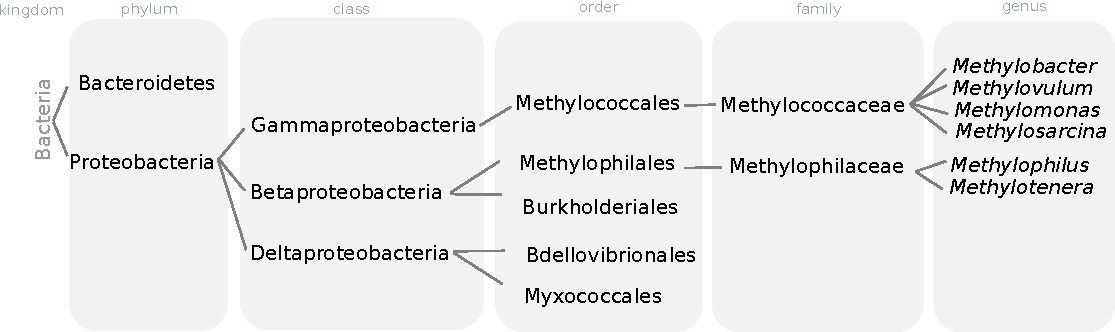
\includegraphics[width=1.0\textwidth]{./tex/chapter2/figures/170311_taxonomy_overview.pdf}
    \begin{singlespace}
    \caption[Taxonomy of microbes known to factor into methane oxidation in Lake Washington sediment]{
       Taxonomy of microbes that often appear in methane incubations of Lake Washington sediment.
       The family \textit{Methylococcaceae} is methanotrophic.
       The family \textit{Methylophilaceae} includes non-methanotrophic methylotrophs.
       Burkholderiales grow on multi-carbon compounds, but in addition, some are methylotrophs.}
    \label{fig:taxonomy}
    \end{singlespace}
\end{figure}

\subsubsection{Goals of this study}
This study aims to identify the major methanotrophic, methylotrophic, and other microbial species that together enable methane consumption in Lake Washington, and deduce each taxa's contribution to the community metabolism.
Identification of which methanotrophs dominate in natural communities provides insights into how good past isolate studies reflect the true drivers of methane oxidation.
Identification of which metabolic pathways are expressed by these methanotrophs and the accompanying non-methanotrophs informs the mechanism of methane oxidation in this natural system.
Understanding the contribution of each microbe to the community metabolism allows hypotheses about genetic factors in methanotroph/methylotroph partnerships.

%For example, this study also aims to address the relative importance of two functionally redundant methanol dehydrogenase enzymes: Xox-MDH and Mxa-MDH. (cite).
%TODO: write more about this if I get results in the area.
%TODO: Some methylotrophs only have Xox.  So they are using it, or absent.

% --- How this dataset is poised to address these questions:    Experimental design: (don't make it too methodsy!)
The experimental design chosen to answer these questions is show in in Figure \ref{fig:experimental_design}.

\begin{figure}[H]
\centering
    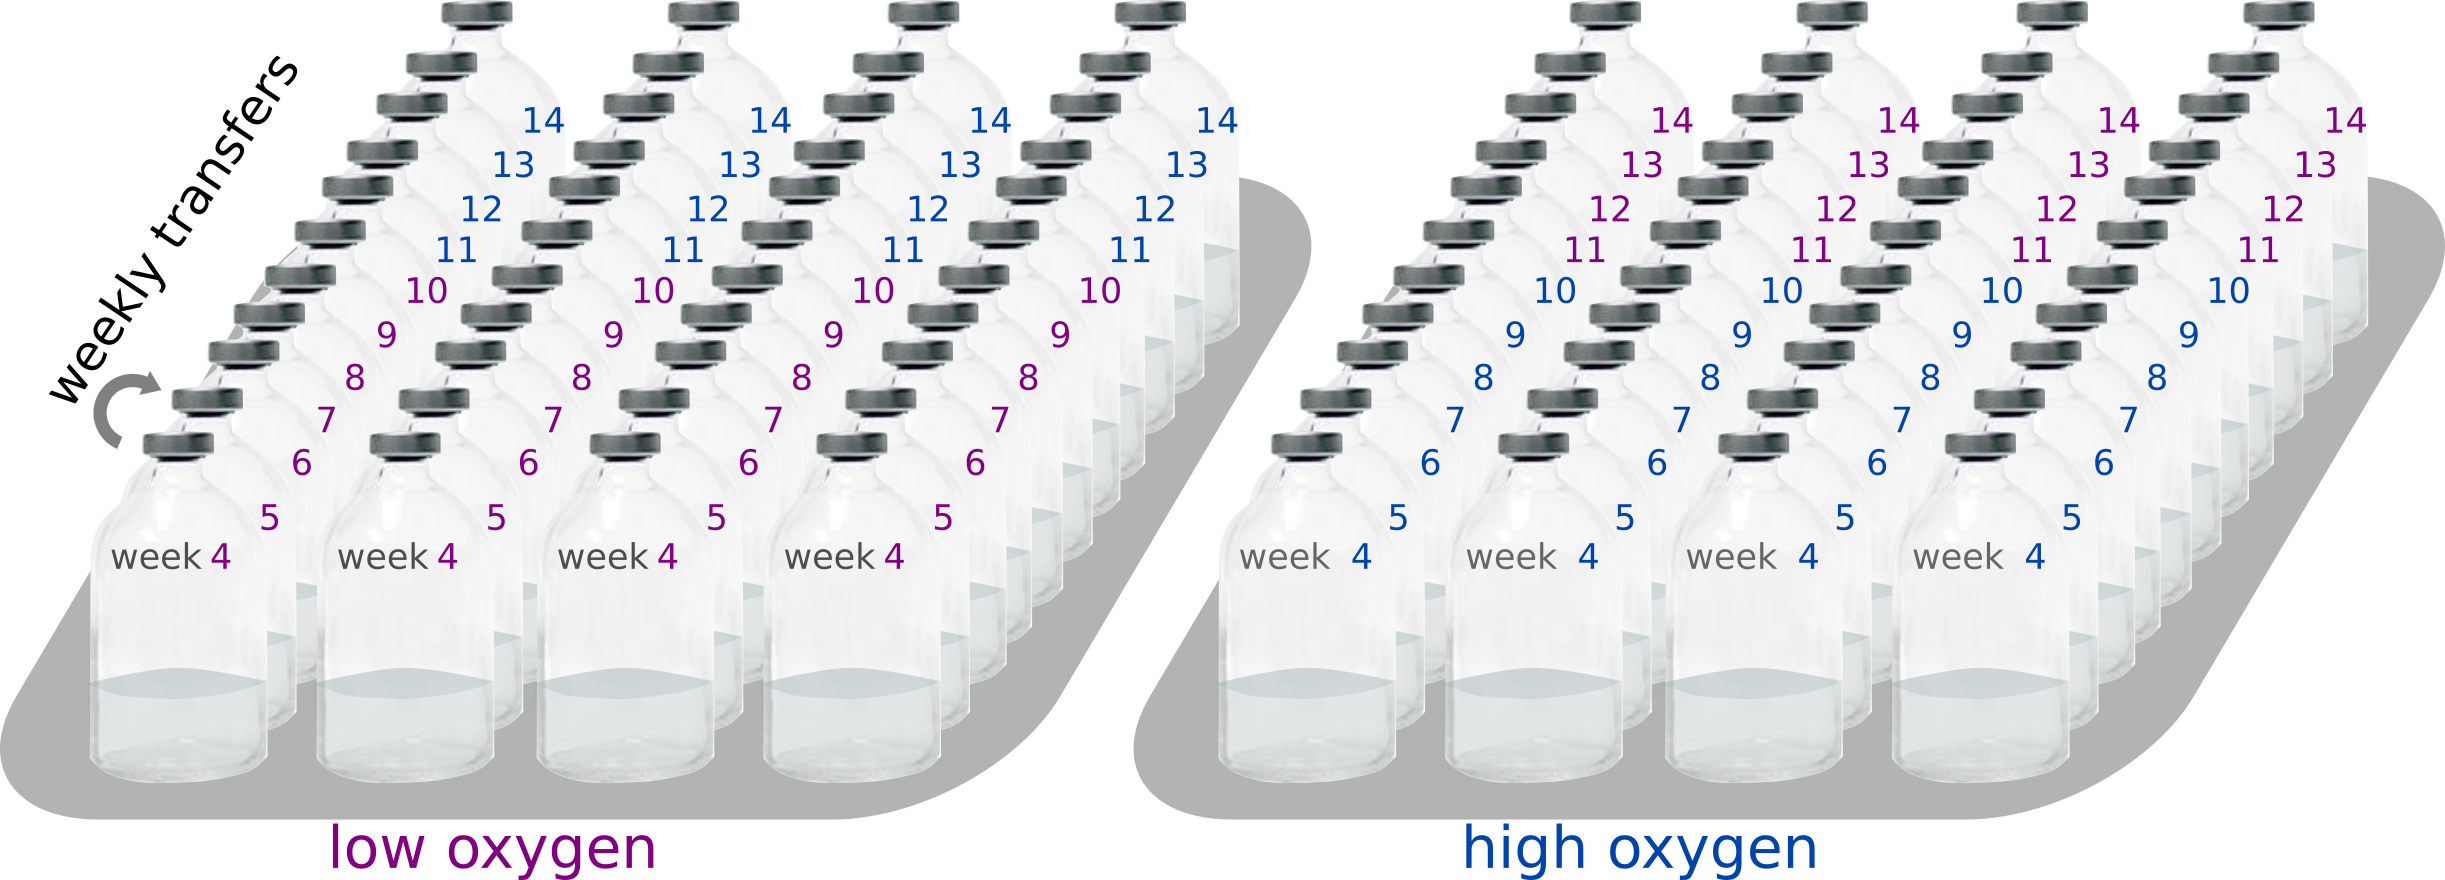
\includegraphics[width=1.0\textwidth]{./tex/chapter2/figures/170311_experimental_design_meta4--2_colors.png}
    \begin{singlespace}
    \caption[Experimental design for the data underlying Chapters \ref{chapter:A} and \ref{chapter:B}]{
	Experimental design for the data underlying Chapters \ref{chapter:A} and \ref{chapter:B}.
	Sediment from Lake Washington was thawed from -80$^o$C and cultured in 8 different bottles,
        half of which were provided with low oxygen, and half of which were provided with high oxygen (see methods).
	   Bottles were serially transferred for a total of 14 weeks.
	   The last four bottles in each series are at the opposite oxygen condition of the original experimental design
        (indicated by bottle label color switch).
	   Metagenomes and metatranscriptomes were obtained for weeks 4-14, resulting in 88 metagenomes and 88 metatranscriptomes.
	   }
    \label{fig:experimental_design}
    \end{singlespace}
\end{figure}

This relatively simple experimental design, including high degree of replication for studies of this type, was chosen to provide statistical power despite differences across replicates and measurement noise.
Variation across replicates can arise from stochasticity as communities rarefy, and are compounded by the noise-generating steps of nucleic acid extraction, ribosomal RNA removal (in the case of metatranscriptomics), library prep, and the sequencing process.
The most important environmental variable identified in previous studies, the oxygen availability, was modulated while holding all other variables constant.
Availability of sequenced isolate strains from the very ecosystem enhance exploration of the dataset by providing some ground-truth.
Lake Washington isolates can also be integrated into positive controls for many of the computational methods.

% --- Data sets like this are rare and special.
Though sequencing has become routine in most biological domains, this dataset is exceptional for several reasons.
Having four replicates for each experimental condition is much greater than typical metagenomic studies.
Furthermore, most metagenomics/metatranscriptomics studies are single time point snapshots, rather than time-series.
Having 11 samples in each series leads to a total of 88 samples.
For each of the 88 samples, untargeted metagenomes and metatranscriptomes were gathered.
These pairs allow exploration of the community without the restriction of referencing cultured strains' genomes.
Ribosomal RNA was depleted, so the majority of the information in the transcriptomes derives from mRNA.
In all the dataset totals to 9TB.

% --- Insights into what's challenging
Despite the size and replication of this dataset, answering the questions outlined above proved challenging.
First, the study aims to answer who is there, without the luxury of using reference DNA to align sequencing data to.
Thus, the first task is to assemble reference DNA from the vast number of short sequences provided.
This DNA then becomes the basis for answering both "who is there", and the reference for "what are they doing".
Ideally, the assembly yields a small number of long sequences.
More often than not, however, under-sampling of DNA or lack of punctuation in well-sampled (highly abundant) strains leads to fragmented reference DNA.
This fractured reference DNA carries uncertainty and information loss through the rest of the analysis, so care must be taken when interpreting all downstream results (see Figure \ref{fig:pipe_leaks}).

% -- Tool selection & evaluation is challenging.
Tool selection and evaluation is also challenging.
As discussed in the introduction, metagenomics and metatranscriptomics of natural microbial communities is a rapidly developing field laden with methodological challenges.
For each step of inference, there are numerous tools to choose from.
Some understanding of the underlying methods is necessary for prudent selections.
Given that each tool has different efficacy for different data sets, several tools are usually tried for each step.
For each tool, there are numerous settings the authors encourage users to tune, leading to a combinatorial explosion of potential outcomes for each inference step.
The nearly complete turnover of tools approximately every 5 years leads to very few benchmarking studies, and review papers that are out date within months of publication.
Furthermore, benchmark studies comparing tools use a small number of data sets that may not behave like your own data set.
%Methods and metrics for tool evaluation are not standardized. repeated below

% --- Lack of standards in field
The field also lacks standards for assessing the efficacy of each inference step.
This is in part due to differences in goals across metagenomics/metatranscriptomics studies: some aim for high confidence inference about a specific sub-population such as a novel taxa, whereas others aim to describe the sample more broadly.
Many tools provide only limited insight into their efficacy on your particular dataset.
Care must be taken by the investigators to select the right tools, connect them properly, and evaluate results critically.
Often the trade-offs between tools are not evident until they are tested, and the data is explored with a critical eye.
Success in this field requires iteration as these insights are developed.

% --- So Big!
Furthermore, the size of this dataset is both luxurious and challenging.
Yes, the high degree of replication and number of samples per series is essential for identifying hypotheses in noisy data.
However, many computational tools are not designed to scale to input data of this size, leading to a variety of failure modes. %and fail when used on larger datasets than they were developed for.
%While some fail quickly and with informative messages, other simply fail by running indefinitely without the tool either completing its task or aborting.
%For some goals, the data can be broken into subsets, processed separately, and re-joined upon completion.
%However, not every tool can operate on segments of the data, and extra care is required when stitching together results such that the next tool downstream is blind to such manipulations.
Despite the challenges, this chapter provides a coarse description of which microbes are present, and what they contribute metabolically.
Steps to zoom in on particular microbes to tell more detailed stories about a subset of the population are outlined as future directions.


%==========================================================================================================================================
%==========================================================================================================================================
%==========================================================================================================================================
\section{Metagenomics and Metatranscriptomics}

\subsection{Introduction to Metagenomics and Metatranscriptomic Inference}
Metagenomics and metatranscriptomics are umbrella terms for any project that uses sequencing of mixed populations of organisms.
It implies untargeted sampling of the samples' entire DNA or RNA pool, rather than selecting for specific types of sequences.
This is in contrast to 16S surveys, which amplify DNA from a segment of the conserved bacterial 16S ribosome \cite{kunin2008}.
16S DNA sequences are used as a molecular clocks for large timescales, and allow for inference of the bacterial taxa present in samples.
16S studies do not allow the possibility to determine what genes each organism has available.
Sometimes two organisms are nearly identical at the 16S level, but have substantial metabolic differences due to insertions, deletions, and transposons.  % todo (cite) (tried for 20 min).
The term "metagenomics" is typically reserved for un-targeted sampling of the entire community DNA pool.
Metagenomics affords the possibility of identifying the genetic composition of individual microbes, albeit after much greater analysis efforts.
Prior studies of Lake Washington sediment painted the coarse 16S-based perspective of who is present in Lake Washington's sediment \cite{beck2013LW, hernandez2015LW, oshkin2015LW}, and did preliminary untargeted metagenomics \cite{beck2013LW, oshkin2015LW}.
This work focuses solely on untargeted metagenomics and metatranscriptomics, to address the more challenging questions of microbial genetic composition, and the associated gene expression levels. % to provide a basis for expression analysis.

%---- Isolates vs de-novo reference-free assemblies.
Once shotgun metagenomic samples are in hand, there are many possible ways to infer which organisms are present and what they express.
One approach is to assess how the samples relate to isolate organisms, by mapping to the reads to the isolates' genomes.
High mapping rates to an isolate genome suggests the sample contained a large abundance of a similar organism.
Given enough similarity, mapping of DNA and RNA reads to these genomes can inform the abundances and expression patterns for organisms in the samples.
This strategy is only effective if the isolate genomes accurately represent strains in the community.
%This can afford an excellent benchmark for analysis of metagenomes or transcriptomes, but only if the isolate genomes accurately represent the strains and diversity of strains in the community sample.
Isolates are often poor proxies for natural microbes given that the vast majority of isolates are not currently culturable \cite{kaeberlein2002, stewart2012}.
Even if the isolates are perfect proxies for some organisms, the set may be missing whole categories of other organisms.
This project did a preliminary study using isolate genomes as a reference for mapping metatranscriptome reads, but discovered that only a small fraction of the RNA mapped to the genes in the isolate genomes (Figure \ref{fig:isolate_RNAseq}).
The project quickly pivoted to reference-genome-free workflows, whereby the metagenomic reads were assembled into contigs that collectively represent the DNA present in the dominant and semi-abundant microbes.
These contigs can be annotated to identify genes, and organised into genome bins intended to represent single strains or groups of highly similar strains.

\begin{figure}[H]
\centering
    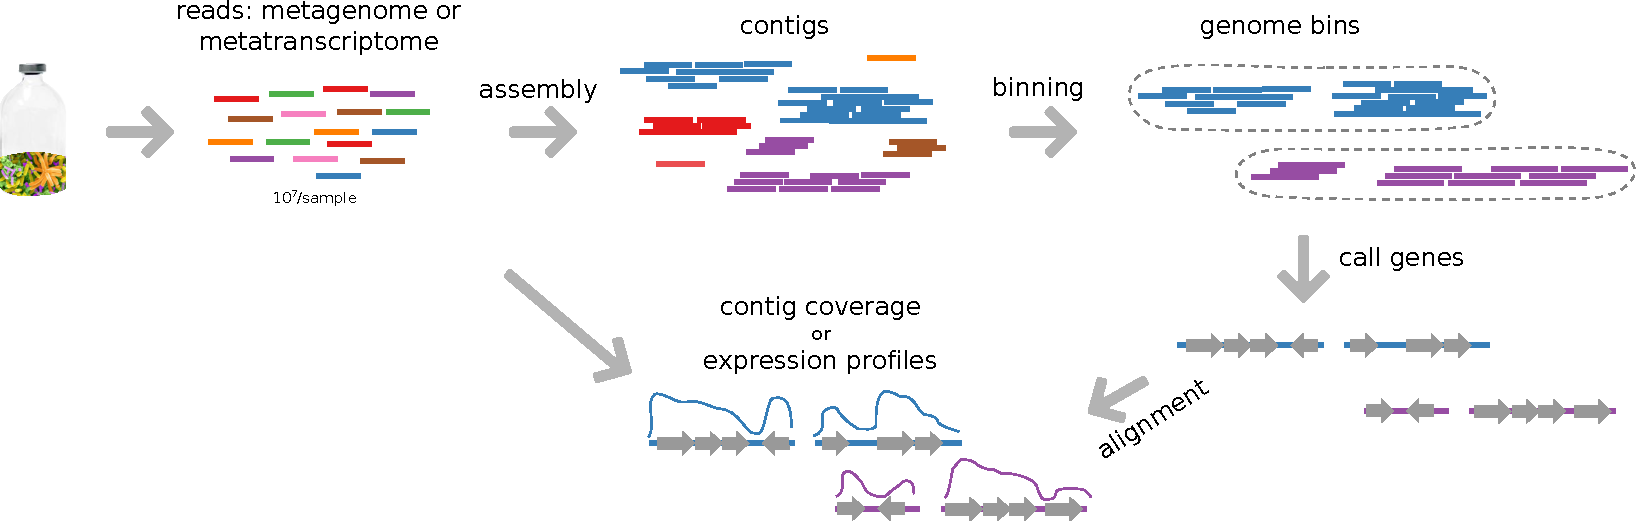
\includegraphics[width=1.0\textwidth]{./tex/chapter2/figures/170312_metagenomics_metatranscriptomics_overview.pdf}
    \begin{singlespace}
    \caption[Overview of elements in metagenomics/metatranscriptomics workflows]{
       Graphical introduction to basic vocabulary and inference steps of metagenomics and metatranscriptomics workflows.
	   Short colored lines = single reads, long colored lines = contigs,
	   gray arrows on top of colored lines = gene calls, wiggly lines above contigs depict the coverage of an alignment.}
    \label{fig:meta_workflow}
    \end{singlespace}
\end{figure}

A simplified representation of steps common to most shotgun metagenomics papers is depicted by Figure \ref{fig:meta_workflow}.
The first step of reference-free metagenomics is assembly, wherein contigs are aligned and fragments are merged to infer the sequence from which the reads originated.
Binning aims to identify contigs that in aggregate represent single organisms, or groups of highly related organisms \cite{kunin2008}.
Genes can be called on the contigs, either before or after binning, to reveal the genetic potential of the organisms.

The flow of information through metagenomics pipelines can be thought of as liquid flow through piping with leaks (Figure \ref{fig:pipe_leaks}).
In the process of aggregating information, each software step can lose information ("leak") along the way.
Flow (read accountability) can be measured at the input and exit of pipes (represented by flow gauges), allowing identification of how well output data reflects the original samples, and at which step(s) information was lost.

\begin{figure}[H]
\centering
    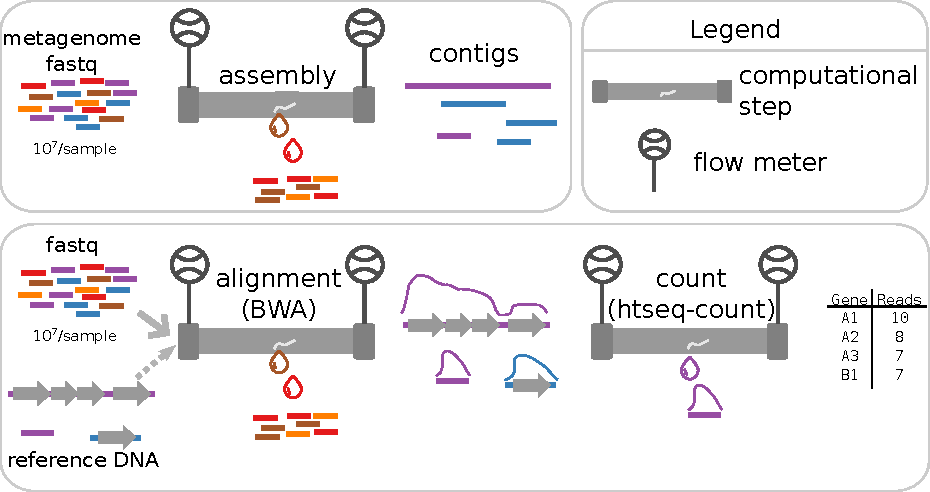
\includegraphics[width=0.8\textwidth]{./tex/chapter2/figures/170312_pipe_leaks.pdf}
    \begin{singlespace}
    \caption[Framework for assessing information loss in workflow steps]{
        Cartoon representing the ability to deduce information loss at different steps of the metagenome/metatranscriptome work flow.}
    \label{fig:pipe_leaks}
    \end{singlespace}
\end{figure}

%---- Pipe description
%A simplified cartoon of the framework used to assess efficacy of each tool in the work flow is illustrated by Figure \ref{fig:pipe_leaks}.
For papers where the goal is to describe one or several novel organism(s) with high confidence, the loss of information (reads) along the way may not be a significant concern.
Often papers in this category do not clearly report an estimate of the identified organisms' abundance in the natural community.
% Don't trash other papers \cite{evans2015} , or obscure absolute abundances by using relative abundances \cite{daly2016}.
Other papers try to describe a more wholistic description of the community (e.g. \cite{kantor2017}) by describing the diversity of organisms identified via binning.
In this case, it is crucial to quantify what fraction of the original sample is described by the output of the computational analysis.
These statistics are usually not stated clearly, allowing readers to over-estimate the importance of the described taxa in the ecosystem.
% At this stage, or research is in this camp, and the result section will highlight how this frame of mind guided selection of tools.
The pipe analysis framework illustrates the approach of this paper: use multiple monitoring methods to determine which pipeline steps are associated with information loss.
These statistics are assessed throughout to prevent misinterpretation of claims about community compositions and expression patterns.
%This thesis aims to describe the community wholistically, and thus strives to clearly report assembly, binning, and read mapping efficacy so as to not overstate claims or exaggerate community simplicity.
% Many literature studies report small and incomplete descriptions about efficacy of their assembly and binning, which obfuscates leaks in the analysis pipeline and corresponds to over-simplified descriptions of the environment under study.  % Don't cite: hard to be certain I read carefully enough to call out papers by name.  It's also not nice!

%----- There is no road map!
Each computational step can be executed by several or sometimes dozens of competing software packages \cite{sangwan2016,thomas2012}.
Each tool can report basic statistics about efficacy based on inputs and outputs, but it it up to the researcher with larger-scope understanding of the project goals to write scripts to critically assess efficacy of the tools in aggregate.
Results from one software package can give you better insight about how to evaluate the other packages' results, so an iterative process with various somewhat-equivalent tools can maximize accuracy.

Another challenge of projects of this scope is the size of the data.
While more data can lead to greater potential for extracting information from uncertain data, many tools are not designed to work on sequencing data as large as these.
While some tools fail quickly and with informative messages, other simply fail by running indefinitely without the tool either completing its task or aborting.
For some goals, the data can be broken into subsets, processed separately, and re-joined upon completion.
However, not every tool can operate on segments of the data, and extra care is required when stitching together results so the next tool downstream will be blind to the upstream manipulations.

%Tools choke.  Just don't complete.
%Sometimes the parameters can be altered, sometimes you can break up a dataset and feed it to a tool in pieces, but sometimes the size is a deal breaker.

It is the role of the computational biologist to learn enough about the competing tools to select a handful to try, develop metrics and priorities for the trade-offs of each tool, project complex data into summary graphs, and decide which tool is the best fit for the research goals.

\subsubsection{Assembly}
%---- Why assemble
Analysis of metagenomic and metatranscriptomic data usually beings with assembling metagenome reads into contigs (Fig \ref{fig:meta_workflow}), which are contiguous stretches of genomic sequence in which the order of bases is known to a high confidence level. %(JGI)
The metagenomes can be aligned to these contigs to infer the abundance of organisms.
The transcriptomes can be aligned to these same contigs to infer what genes are expressed.
In principle, metagenomes and metatranscriptomes can be aligned to isolate genomes rather than contigs, however, in practice meta-omics experiments are usually used precisely when the isolates available are known to be incomplete representatives of the microbial community under study.
Even if a similar organism has been isolated, the investigation may be probing the diversity of similar organisms, or the influence of less abundant microbes on the community's function.

%---- Not all assemblies are created equal
The challenge of assembly scales with the complexity of the microbial community.
High species diversity and strain-level heterogeneity add challenge to assembly \cite{kunin2008, thomas2012}.
Communities with a small number of well-delineated species tend to assemble better, yielding shorter numbers of long contigs.
In contrast, complex communities' high diversity can lead to fragmented assemblies, having fewer long contigs and more short contigs \cite{kunin2008}.
These shorter contigs are more challenging to analyze and can lead to an incomplete portrait of a community.
Short contigs are more difficult to call genes on, and are also more difficult to bin because measures like GC and differential abundance are noisier for short contigs than long ones \cite{sangwan2016}.
The most common measures of assembly efficacy are characteristics of the contigs themselves.  How many are there?  What is the length of the contig that divides the length-sorted contigs into a pair of equal lengths (termed "N50")?
This thesis advocates for additional measures that are rarely reported: the fraction of the total (un filtered/trimmed) original reads that map to the assembled contigs, and genome bins.   % todo: "seldom seen" instead of "not seen"?
% Dont' talk about restricting to contigs > 1.5kb.

\subsection{Elviz Assemblies}
%---- JGI assemblies
The sequencing for many metagenomics projects, including this one, are done by the Joint Genome Institute (JGI).
JGI provides some bioinformatics processing in addition to providing un-processed reads.
The software they run assembles contigs for each sample individually, predicts genes, and calls taxonomy for contigs \cite{cantor2015}.
They also report the number of reads and average coverage for each contig.
These measures are a great starting point for answering "who's there" in terms of taxa abundance, but does neglect information about reads that did not assemble well and thus must be used with caution.

%---- Not assembled together
The contigs JGI provides are assembled for each sample, individually.
For this project, that means there are 88 separate assemblies.
Thus the contigs are not shared across samples, and comparison across samples is hindered.
For example, it is difficult to infer whether a particular gene is differentially expressed across two samples if the contigs used as reference DNA are not the same across samples.
More powerful analyses can be done when the DNA from all metagenomic samples are assembled together.
This makes it possible to map DNA and RNA reads back to this shared DNA and thus to tabulate gene expression across samples.
Such an assembly also leads to more powerful binning (discussed below) by providing extra features to cluster with: the differential abundances of each contig across the samples \cite{albertsen2013}.
Since the number of reads originating from a particular organism should be proportional to its abundance, the DNA coverage for a set of contigs originating from an organism should be similar in a particular sample, and correlated across samples.
The per-sample nature of the JGI contigs restricted the types of analyses that data was used for, and motivated generation of co-assembled contigs to represent the entirety of the dataset as discussed below.

\subsubsection{Binning}
%---- Definition & Why
Desire for understanding at organism-level often leads investigators to approximate genomes as best they can from a set of metagenomic contigs.
The phrase "genome bin", often called simply "bin", is used to describe a collection of contigs used to approximate a single organism's genome.
"Bin" implies the collection is expected to be somewhat incomplete and potentially contaminated by DNA of other strains or species.
Bins allow inference of which metabolic pathways are available, and can be used as a reference to map RNA to for quantification of how these genes are expressed.
Higher confidence claims would be possible upon isolation of the organism represented by the genome bin, but laboratory isolates are often not obtainable either due to obligate partnerships with other organisms, or a variety of intolerances to laboratory conditions \cite{stewart2012}.
Binning can be done before or after annotating genes on the contigs, as very few methods use gene calls in the binning process.

%---- Overview of binning tools' strategies
The most common features used to bin contigs include GC content, tetranucleotide frequency, other oligonucleotide frequencies, and differential abundance across samples \cite{sangwan2016}.
Most aim to be effective without needing reference genomes to align to.
% can't find citation for using an isolate as a binning reference.  Only for assembly.  Drop??

%---- Rarefaction, species heterogeneity
The ability to get clean genome bins varies greatly from project to project.
As with assembly, more rarefied samples with low levels of strain heterogeneity are more amenable to binning \cite{kunin2008, thomas2012}, as the contigs are more likely to be long and few in number.
Longer contigs have reduced noise for measurements of GC ratio, tetranucleotide frequency, and differential abundance \cite{sangwan2016}.
This in turn leads to less ambiguity when sorting contigs into respective bins.
Notably, most binning tools are demonstrated on simple communities such as the premature infant gut \cite{sharon2013}.
Thus, the promising assembly quality statistics noted in binning method papers are not guaranteed to translate for analysis of high-complexity samples such as those in this thesis.
% In fact, most binning methods were demonstrated using relatively simple communities (e.g., premature infant gut datasets of Sharon et al.

%---- Bin assessment
The quality of bins can be determined using metrics of completeness, contamination, and efficacy of representing the sample.
Completeness and contamination checks can be automated by use of CheckM \cite{parks2015}, which uses the presence of marker genes in each bin as the basis for its approximations.
The marker genes used by CheckM are different based on the approximate taxonomy CheckM infers for the bins.
While this is certainly more effective than one set of genes used for all microbes, the reference sets available may not be good fits for the particular microbes under study.
Furthermore, the choice of reference gene sets might be poor for messy bins that contain contigs from wildly different taxa.
Some papers determine completeness and contamination by manual inspection using domain-specific marker gene sets. % (cite)
For papers published before CheckM, this manual check was the best option.
Now CheckM is used in the majority of papers.
It even allows the possibility of adding custom marker gene sets for CheckM to use.

%---- Binning tools
The binning tools used herein combine sequence composition and coverage across multiple samples as inputs to machine learning algorithms that automatically cluster contigs into genomes.
Several were tried, given that differences in their algorithms and output characteristics are seldomly and vaguely reported \cite{sangwan2016}.
Metabat \cite{metabat2015} uses k-medoid clustering of a distance measure composed of tetranucleotide frequency and abundance.
% ** doesn't use marker genes **
MyCC \cite{mycc2016} uses affinity propagation to cluster contigs, and uses the presence of marker genes to correct clusters.
%"an automated binning tool that combines genomic signatures, marker genes and optional contig coverages within one or multiple samples"
%"FetchMG extracts 40 universal phylogenetic marker genes"
%"AP-generated clusters were finally corrected based on the sequences harboring marker genes"
CONCOCT \cite{concoct2014} uses a Gaussian mixture model fit with a variational Bayesian approximation, on features thinned out via principle components analysis (PCA).
% This says it uses marker genes, but the original paper doesn't mention it.
% Manual curation
Almost every high-quality bin published in high-profile papers has used tools such as these, but the resulting bins are subsequently refined by manual curation, with methods only vaguely described.

\subsubsection{Mapping RNA}
Metatranscriptomes can be mapped to contigs or bins.
A key variable to consider is what you want to happen with reads that map to multiple places.
If a read maps equally well to two different contigs in a bin, should it be randomly assigned to one locus, or thrown away?
If the study is aiming for differential expression type analysis, than the latter is better.
Discarding ambiguous reads is the default of most alignment and counting tools.
If the study aims to describe a wholistic picture of expression in a sample, it may be worth guessing the source of multiply mapped reads.
Special care must be taken after that step, as the estimates will certainly be wrong some of the time.


%==========================================================================================================================================
%==========================================================================================================================================
%==========================================================================================================================================
\section{Methods}

\subsubsection{Experimental}  % Note that work was done previously, so I'm not implying I did it.
The culturing and sample preparation was done by Maria Hernandez, a visiting scholar.
Sediment stored in an aqueous DMSO solution on previous sampling trip was thawed from -80$^o$C and distributed into 250 mL bottles containing 100mL of NMS medium \ref{fig:experimental_design}, leaving 150mL of headspace.
% High: 75% air, low = 75% air.  150 mL headspace, 100 mL liquid.
All bottles were air-tight, with head spaces containing 25\% methane.
High oxygen samples' head space was 75\% air.
Low oxygen samples' head space was 15\% air, with the remainder being nitrogen.
Atmospheres were created every weekday and once per weekend.
Bottles were shaken at 250 RPM and held at 18$^o$C.
The gaseous compositions for the days between transfers were not measured.

Bottles were serially transferred for 14 weeks.
Metagenomes and metatranscriptomes were obtained for all samples corresponding to weeks 4-14.
Earlier weeks were omitted due to potential effects of residual DMSO, and interest in prioritizing sequencing of later, more-rarefied samples.
The oxygen conditions (low/high) were switched for the last 4 bottles in each series (see Figure \ref{fig:experimental_design}).

\subsubsection{Sequencing}
This large dataset was made possible by a Joint Genome Institute sequencing grant. % (cite the \#? XX).
JGI sequenced all samples on an Illumina platform to produce the 88 metagenomes and 88 metatranscriptomes.
Ribosomal RNA was removed before sequencing the metatranscriptomes.
%~ XX (?? Paired ended?) reads per sample, for both metagenomes and metatranscriptomes (??).

\subsubsection{Elviz Analysis}
Along with raw sequencing outputs (\texttt{fastq.gz} files) for each sample, Elviz data \cite{cantor2015} was provided by JGI.
These data included one assembly per metagenome, corresponding contig statistics, and transcriptome alignment statistics.
In addition, they provide taxonomy for each contig, to some degree of certainty: some contigs' taxonomy stops at family, while others are specified to the genus level.
The taxonomy, contig lengths, and number of reads mapped to each contig were used to infer the distribution of taxa in each sample.
The metric used was the fraction of reads assigned to contigs with the specified taxonomy (code at \url{https://github.com/JanetMatsen/elvizAnalysis/blob/master/abundance_utils.py}).
Length of contigs was not normalized out, or the abundance of short contigs would dominate the results.
The code checks that the taxas` abundances summed to 1 for each sample.

Tools were written to aggregate (a) based on taxonomy level, or (b) everything below a taxonomy level.
Contigs with taxonomy not described to the specified level were grouped into "unknown \& other".
This framework was also used to summarize abundances at mixed taxonomy level (e.g. phylum Bacteroidetes, order Burkholderiales, family \textit{Methylococcales}, and family \textit{Methylophilales}), and plotted (code: \url{https://github.com/JanetMatsen/elvizAnalysis/blob/master/abundance_plot_utils.py}).

Statistics for the 88 samples were merged with information about the oxygen, replicate, and week values corresponding to each sample using Python and Pandas.
Plotting was done with Matplotlib, Pandas, and Seaborn.

\subsubsection{Computational resources}
This computationally-intensive research was supported by an AWS research grant, which included \$27k of compute resources and expert consulting on how to best utilize the vast services offered.
AWS allows per-hour rental of machines with different specifications, that the user can choose based on algorithm needs.
Furthermore, the ability to share machine images with other researchers greatly facilitates the potential reproducibility of research.
Upon project completion, an Amazon Machine Image (AMI) encapsulating the entire data analysis pipeline will be provided so others can re-run our analyses.

The machine ("instance") type used in all methods to follow was an AWS EC2 c4.8xlarge instance, which has 36 cores and 60GB memory.
This was sufficient for all work, other than the memory-intensive assembly step, as noted below.
Instances could be turned on and off as needed, reducing compute costs.
This is in contrast to sharing a similar machine with an entire research lab, which would have slowed down analysis and caused conflicts when certain computations used all of the compute resources, sometimes causing computer failure.

Each instance obtained data and wrote results to a shared file system.
The 9 TB of data, scripts, and results were stored using the AWS Elastic File System (EFS).
EFS is currently AWS's most versatile and highest performance (most expensive) file storage, which allows users to have multiple instances reading/writing to the same directory.
This shared nature of the files allows the user to spin up a second computer instance as needed, and do read/write operations on the exact same set of files.

%---- Computation parallelization
Parallelization of compute tasks was done by splitting jobs across a single large computer, or across separate EC2 instances.
When tasks were parallelized across one powerful computer, Gnu parallel or Python's \texttt{pool.map} were used.
When parallelizing across more, often weaker, computers, an AMI was made that mounts the EFS-stored data.
These instances were usually started by hand through the console, though proof of principle studies using the Amazon Command Line Interface (CLI),
    and an Autoscaling/SQS service pair were explored to set the foundation of future work (see repository \url{https://github.com/JanetMatsen/AWS_parallel_Cowsay}) for the templates developed.

\subsubsection{Map to isolate genomes}
As a preliminary study, the metatranscriptomes were mapped to 55 genomes (Table \ref{table:55genomes}) isolated from Lake Washington by the Lidstrom Lab.
The sequences were downloaded from NCBI, and concatenated together before mapping.
Mapping to the multi-fasta rather than the individual genomes prevents double-counting of reads that map well to multiple loci.
BWA-MEM \cite{li2009} with default settings was used to map each transcriptome to the multi-fasta, and htseq-count \cite{anders2014} was used to tabulate expression estimates.
Samtools \cite{li2009samtools} was used to evaluate mappings produced by BWA-MEM.
Note: the default of BWA-MEM is to flag reads that map equally well to two or more loci as having quality score 0; htseq-count by default omits these counts from the table of reads per gene (discussed later).

\begin{singlespace}
\begin{longtable}{p{.50\textwidth}}
\caption[The 55 isolate genomes used]
	{The 55 isolate genomes used.}
\label{table:55genomes}
\endfirsthead
\endhead
\midrule
               \textit{Ancylobacter} sp. FA202 \\
                 \textit{Arthrobacter} sp. 31Y \\
                 \textit{Arthrobacter} sp. 35W \\
               \textit{Arthrobacter} sp. MA-N2 \\
                    \textit{Bacillus} sp. 37MA \\
                      \textit{Bacillus} sp. 72 \\
                        \textit{Bosea} sp. 117 \\
                \textit{Flavobacterium} sp. 83 \\
                \textit{Flavobacterium} sp. Fl \\
                      \textit{Hoeflea} sp. 108 \\
               \textit{Hyphomicrobium} sp. 802 \\
                \textit{Hyphomicrobium} sp. 99 \\
           \textit{Janthinobacterium} sp. RA13 \\
    \textit{Methylobacter tundripaludum} 21/22 \\
    \textit{Methylobacter tundripaludum} 31/32 \\
              \textit{Methylobacterium} sp. 10 \\
              \textit{Methylobacterium} sp. 77 \\
             \textit{Methylobacterium} sp. 88A \\
                \textit{Methylocystis} sp. LW5 \\
                 \textit{Methylomonas} sp. 11b \\
                \textit{Methylomonas} sp. LW13 \\
                 \textit{Methylomonas} sp. MK1 \\
        \textit{Methylophilaceae bacterium} 11 \\
                 \textit{Methylophilus} sp. \#1 \\
                 \textit{Methylophilus} sp. 42 \\
                  \textit{Methylophilus} sp. 5 \\
                 \textit{Methylophilus} sp. Q8 \\
                  \textit{Methylopila} sp. 73B \\
                 \textit{Methylopila} sp. M107 \\
            \textit{Methylosarcina lacus} LW14 \\
                 \textit{Methylosinus} sp. LW3 \\
                 \textit{Methylosinus} sp. LW4 \\
                 \textit{Methylosinus} sp. PW1 \\
            \textit{Methylotenera mobilis} \#13 \\
           \textit{Methylotenera mobilis} JLW8 \\
               \textit{Methylotenera} sp. 1P/1 \\
                \textit{Methylotenera} sp. 73s \\
                \textit{Methylotenera} sp. G11 \\
               \textit{Methylotenera} sp. L2L1 \\
                \textit{Methylotenera} sp. N17 \\
          \textit{Methylotenera versatilis} \#7 \\
        \textit{Methylotenera versatilis} 301, \\
          \textit{Methylotenera versatilis} 79 \\
           \textit{Methyloversatilis} sp. FAM1 \\
       \textit{Methyloversatilis} sp. RZ18-153 \\
   \textit{Methyloversatilis universalis} FAM5 \\
 \textit{Methyloversatilis universalis} Fam500 \\
   \textit{Methylovorus glucosetrophus} SIP3-4 \\
                \textit{Mycobacterium} sp. 141 \\
                \textit{Mycobacterium} sp. 155 \\
                    \textit{Paracoccus} sp. N5 \\
               \textit{Pseudomonas} sp. 11/12A \\
                 \textit{Xanthobacter} sp. 126 \\
                  \textit{Xanthobacter} sp. 91 \\
     \textit{Xanthobacteraceae bacterium} 501b \\
\midrule
\end{longtable}
\end{singlespace}


\subsubsection{Assembly} % (Dave)
Assembly to produce contigs was done on pooled quality-trimmed metagenome reads via Megahit \cite{li2015}.
This memory-intensive computation was done on an AWS instance with 1 TB of memory.
Assembly of multiple samples simultaneously provides a shared set of contigs to use when mapping DNA reads or RNA-seq reads from any of the 88 samples.  % Not methodsy?  Take out?  TODO
This in turn allows for comparison of gene expression across samples.
The fraction of reads represented by the assembly, in aggregate, were measured to verify assembly efficacy.
%Tune knobs until ...
%Followed protocol ...

\subsubsection{Gene calls}
Genes were called on contigs with length greater than or equal to 1.5kb using Prokka \cite{seemann2014} (scripts: \href{https://github.com/BeckResearchLab/meta4/blob/master/m4b_binning/assembly/prokka/prokka.py}{Python script} that calls Prokka, \href{https://github.com/BeckResearchLab/meta4/blob/master/m4b_binning/assembly/contigs_by_length/select_contigs_by_size.py}{script} that extracts contigs by size).
This cutoff was selected because shorter contigs are not recommended for inclusion by most binning tools documentation.
Additionally, shorter contigs are less likely to have genes identified on them, as genes are more likely to be incomplete due to a higher density of contig edges.
Prokka did not tolerate an input size of the scale, so the input fasta was broken into 5 files of approximately equal size (\href{https://github.com/BeckResearchLab/meta4/tree/master/m4b_binning/assembly/prokka/contigs}{scripts}).
These were processed in parallel, using Python's \texttt{pool.map}.
A \href{https://github.com/BeckResearchLab/meta4/blob/master/m4b_binning/assembly/prokka/contigs/glue_together_gffs.py}{script} was written to merge the resulting annotated "general feature format" files (\texttt{.gff} files) into one representing all contigs $\geq$ 1.5kb.

\subsubsection{Checking contigs' ability to represent each metagenome}
The loss of information resulting from omitting short contigs was assessed by counting the number of reads that map to contigs $\geq$ 1.5kb, and comparing that to the total number in the raw metagenome \texttt{fastq.gz} files (\href{https://github.com/BeckResearchLab/meta4/blob/master/m4b_binning/assembly/data/sample_info/count_reads_in_each_sample.sh}{\texttt{.fastq} read counting script}, \href{https://github.com/BeckResearchLab/meta4/tree/master/m4b_binning/assembly/assess_sample_mappings_to_contigs}{analysis}).
This represents an upper bound in information content for the assembly step.
Again, this used BWA-MEM \cite{li2009}, and a \href{https://github.com/BeckResearchLab/meta4/blob/master/m4b_binning/assembly/data/sample_info/count_reads_in_each_sample.sh}{script} written to count reads in \texttt{.fastq} files.
Pandas (Python) was used to merge results together.

\subsection{RNA-seq: mapping to contigs $\geq$ 1.5 kb}
Like all other read mapping steps, transcriptomes were mapped with BWA-MEM (default settings), and per-gene results were summarized with htseq-count.
Contigs $\geq$ 1.5kb were used as reference DNA.
Metatranscriptomes were mapped to these contigs all at once, rather than to each bin individually in order to reduce over-counting.
This does result in reads mapping identically well to two places being thrown out, as mentioned earlier.
Results from each sample were merged using a 60GB RAM AWS instance, rather than SQL.
The fraction of transcriptome reads was compared to the total number in the input \texttt{.fastq} files as a metric of information loss.
See \href{https://github.com/BeckResearchLab/meta4/tree/master/rnaseq/alignments}{scripts and notebook}.

\subsubsection{Binning}

Binning of contigs into genome-like bins was explored using three different packages.
MetaBAT was used with default settings on contigs $\geq$ 1.5kb (\href{https://github.com/BeckResearchLab/meta4/blob/master/m4b_binning/assembly/2.metabat}{script}).
As promised by the documentation, it scaled well to this large dataset. % and completed within about a day.

MyCC was used, but did not scale this large data set.
The large memory requirement of the underlying affinity propagation algorithm led to failures when default settings were used.
At one time, MyCC wrote so many small files that the machine crashed due to running out of inodes.
The authors suggested some alterations to the settings to reduce the computational requirements:  \texttt{56mer, lt 0.4, st 50}.
Use of their settings worked on the set of contigs longer than 2.5kb, but not the larger set of contigs longer than 1.5kb.

Concoct was tried initially, but bins were never obtained.
This tool reports multiple potential clusters per conitg.
The approach for resolving that conflicting information was not sorted out in the time frame of this project.

\subsubsection{Average Nucleotide Identity}
Average nucleotide identity (ANI) was used to compare bins.
The underlying tool, provided by JGI  \cite{varghese2015} (\href{https://ani.jgi-psf.org/html/anicalculator.php}{download link}), calculates two-way global ANI measures and reports the fraction of each genome that aligned.
The authors suggest removal of ribosomal RNA genes, which can have high ANI even for divergent organisms.
They do not, however, provide options or suggest a tool for this step.
Given that the ANI calculations intended only to give a rough idea of similarity between bins or bins and isolates, this step was not performed.
The tool was used to assessed ANI between all pairs of isolate genomes and MetaBAT bins (\href{https://github.com/BeckResearchLab/meta4/blob/master/m4b_binning/assembly/ANI/ANIs_of_all_combos.py}{script}).

\subsubsection{Additional bin characterization}

Completeness and contamination were checked with CheckM \cite{parks2015} (\href{https://github.com/BeckResearchLab/meta4/tree/master/m4b_binning/assembly/bin_info}{scripts}).
CheckM uses marker genes from what it determines to be an evolutionarily similar microbe.
The tool was benchmarked on isolates, to ensure it performed well on the key methylotrophic taxa under study.
Custom marker genes specific to methylotrophs were not added, however, this is suggested as a possible future direction to assess bins.

Taxonomy was approximated using PhyloPhlan \cite{segata2013}, and by ANI similarity with isolate genomes (\href{https://github.com/BeckResearchLab/meta4/tree/master/m4b_binning/assembly/bin_info}{scripts}).

\subsubsection{Code}
The code described was developed with Git version control, and the full history is available on GitHub:
\begin{itemize}
    \item \textbf{ElvizAnalysis}: \url{https://github.com/JanetMatsen/elvizAnalysis}
    \item \textbf{meta4} (assembly, binning, etc.): \url{https://github.com/BeckResearchLab/meta4}
\end{itemize}

%==========================================================================================================================================
%==========================================================================================================================================
%==========================================================================================================================================
\section{Results and Discussion}


%-------- Elviz Analysis
\subsection{Raw Reads}

The cumulative number of raw and un-filtered reads is shown below.
This collection of reads was used for all inferences described in this chapter.
Also see Figure \ref{fig:fastq_reads} for plots showing specific values for each sample.

\begin{table}[H]
% /work/misc/170326_compare_raw_fastq_reads.ipynb
\centering
\begin{singlespace}
\caption[Number of un-filtered reads: sample average and total]
	{Number of un-filtered reads: sample average and total across 88 samples.
	}
\begin{tabular}{l | cc}
 %\toprule
        & mean \# reads per sample & total \# reads \\
\midrule
	metagenomes & \texttt{3.33e+07} $\pm$ \texttt{7.34e+06} & \texttt{2.93e+09} \\ % also from: /work/jmatsen/170308_assess_Elviz_read_attraction_frac
	metatranscriptomes & \texttt{4.24e+07} $\pm$ \texttt{6.22e+06} &  \texttt{3.73e+09} \\
%\bottomrule
\end{tabular}
\label{table:sample_read_sizes}
\end{singlespace}
\end{table}



%-------- Elviz Analysis
\subsection{Elviz Analysis}

The best measure of which taxa dominate the samples comes from the Elviz \cite{cantor2015} data.
As described in the Methods section, the abundance measure was the sum of read counts across contigs labeled with the taxonomy of interest.
Traditional metrics like RPKM \cite{mortazavi2008} and TPM \cite{wagner2012} are excellent for comparing coverage or expression across features or samples, but could not be used due to the need to sum values across contigs.
To illustrate why length of contig could not factor into the abundance measure, consider this:
a contig with length 10kb should contribute nearly identically to an equally expressed second 10kb stretch of DNA that for technical reasons was assembled into two 5kb stretches rather than one 10kb contig.
Any scheme that controlled for contig length or was weighted by each contig's statistic would skew the aggregated number down for metagenomic datasets such as this with many short, low-coverage contigs.
The fact that these assemblies are dominated by short contigs means that RPKM and TPM would bias the aggregate statistics toward the statistics of the shorter and less reliable contigs.
Similarly, median coverage was not used or the unreliable coverage numbers associated with short contigs would dominate the measure.

Figure \ref{fig:4dominant_groups} shows abundances of the four major taxonomic groups, Methylococcales, Methylophilales, Bacteroidetes, and Burkholderiales, according to the Elviz taxonomy calls for each contig. % Methylococcales, Methylophilales are Orders (not italics)
(Recall introductory Figure \ref{fig:taxonomy} for a hierarchical visualization of these taxonomies.)
Their dominance is consistent with pervious studies \cite{beck2013LW, beck2014LW, oshkin2015LW, hernandez2015LW, kalyuzhnaya2008Burkholderiales}.
Figure \ref{fig:dominant_genera} show the breakdown of the methanotrophic and non-methanotrophic methylotroph taxa in Figure \ref{fig:4dominant_groups}.
Notably, the path to rarefaction is not particularly consistent across samples.
Like previous studies, the dominant methanotrophic order/genus was Methylococcales/\textit{Methylococcaceae} and the dominant non-methanotrophic methylotrophic order/genus was Methylophilales/\textit{Methylophilaceae}.
Low oxygen was associated with a higher abundance of methanotrophs, and a lower proportion of methylotrophs than the high-oxygen samples.
\textit{Methylosarcina} is often found in high-oxygen samples, but rarely in low-oxygen samples.
Two high oxygen samples are dominated by \textit{Methylobacter}, but the others are not.
The last four samples in each series are more similar to the previous samples in the series than samples at the opposite oxygen tension.


\begin{figure}[H]
\centering
    % /Users/janet/elvizAnalysis/ipython_notebooks/plots/
    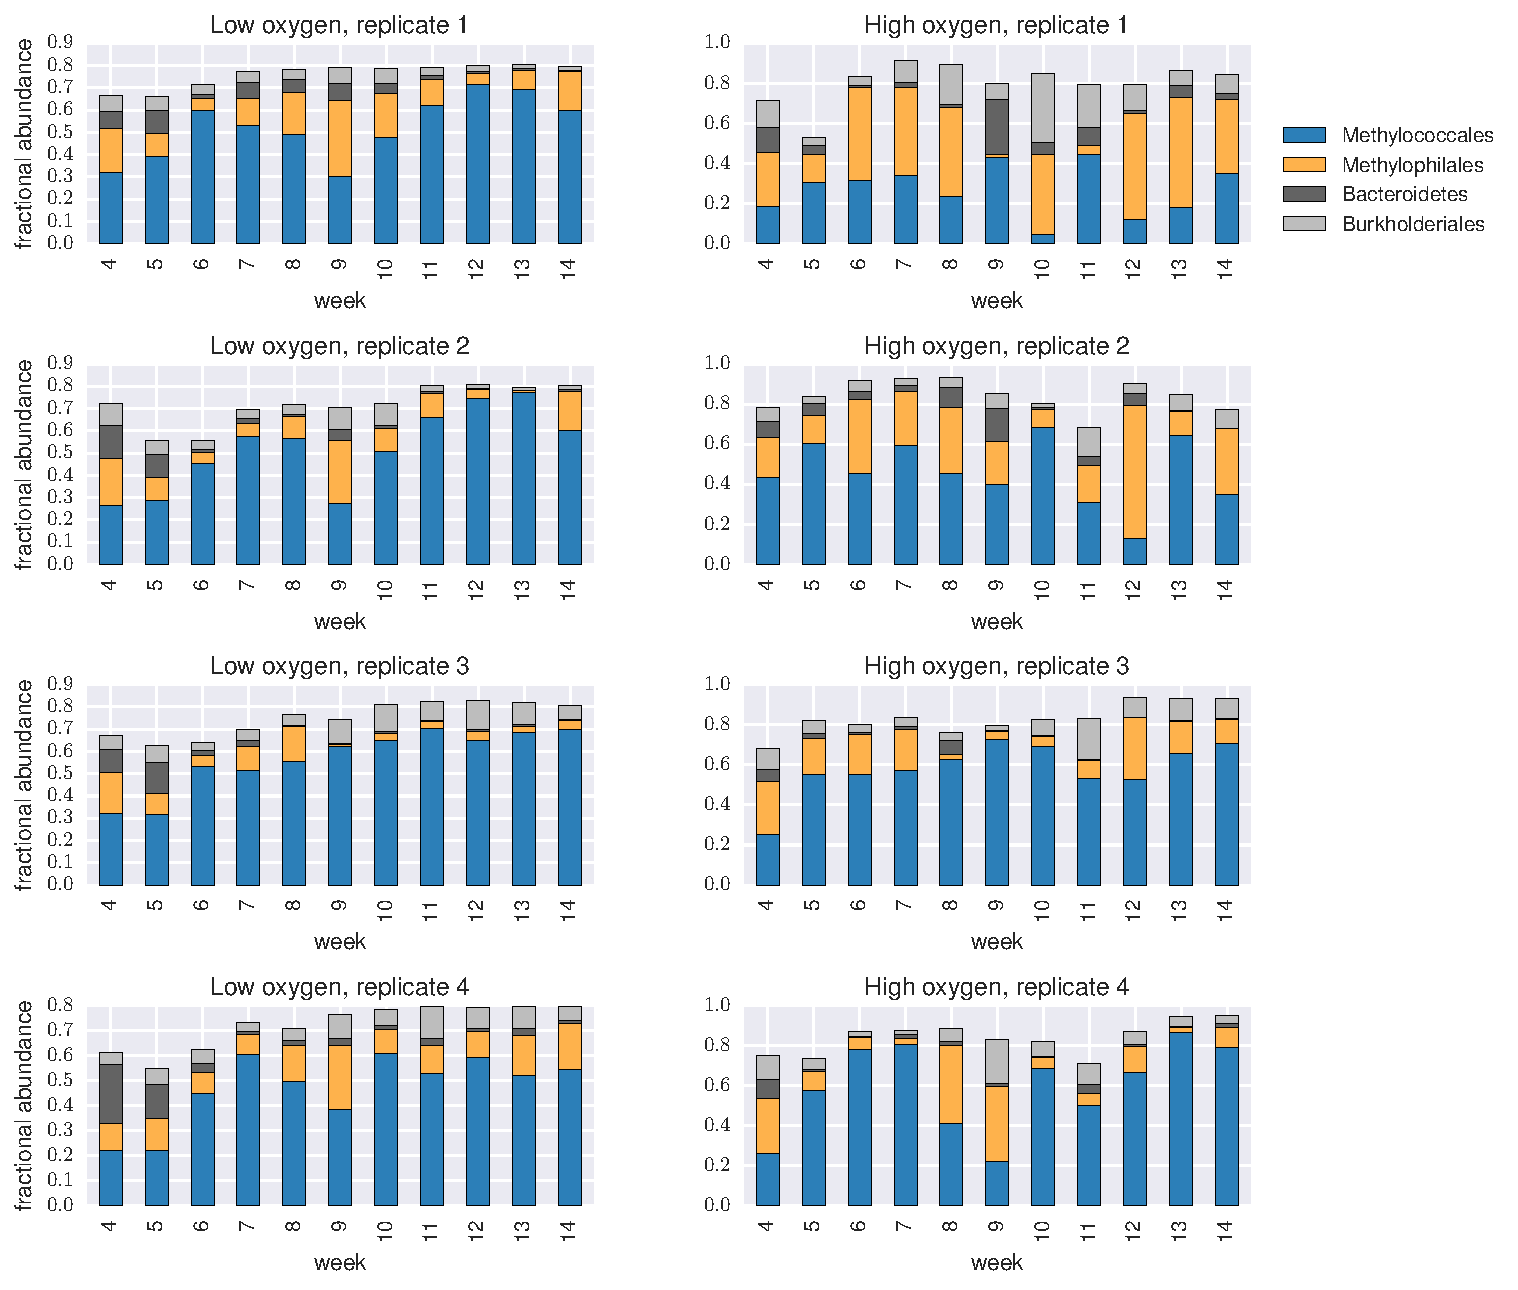
\includegraphics[width=1.0\textwidth]{./tex/chapter2/figures/170413_4_main_groups.pdf}  % ElvizAnalysis
    \begin{singlespace}
    \caption[Four major taxonomic groups in Lake Washington sediment incubations]{
        Fractional abundances of DNA from the four major taxonomic groups in Lake Washington sediment incubations:
	    phylum Bacteroidetes, orders Methylococcales (methylotrophs), Methylophilales (non-methanotrophic methylotrophs), Burkholderiales.
        The vertical gray line indicates the week the oxygen conditions were reversed.
        These bars only reflect reads that mapped to contigs, according to the Elviz pipeline.
        For information about the fraction of reads not assigned to contigs, see Figure \ref{fig:frac_elviz_mapped_to_contigs}.
        }
    \label{fig:4dominant_groups}
    \end{singlespace}
\end{figure}

\begin{figure}[H]
\centering
    % /Users/janet/elvizAnalysis/ipython_notebooks/plots/170313_methanotroph_methylotroph_taxa--portrait.pdf
    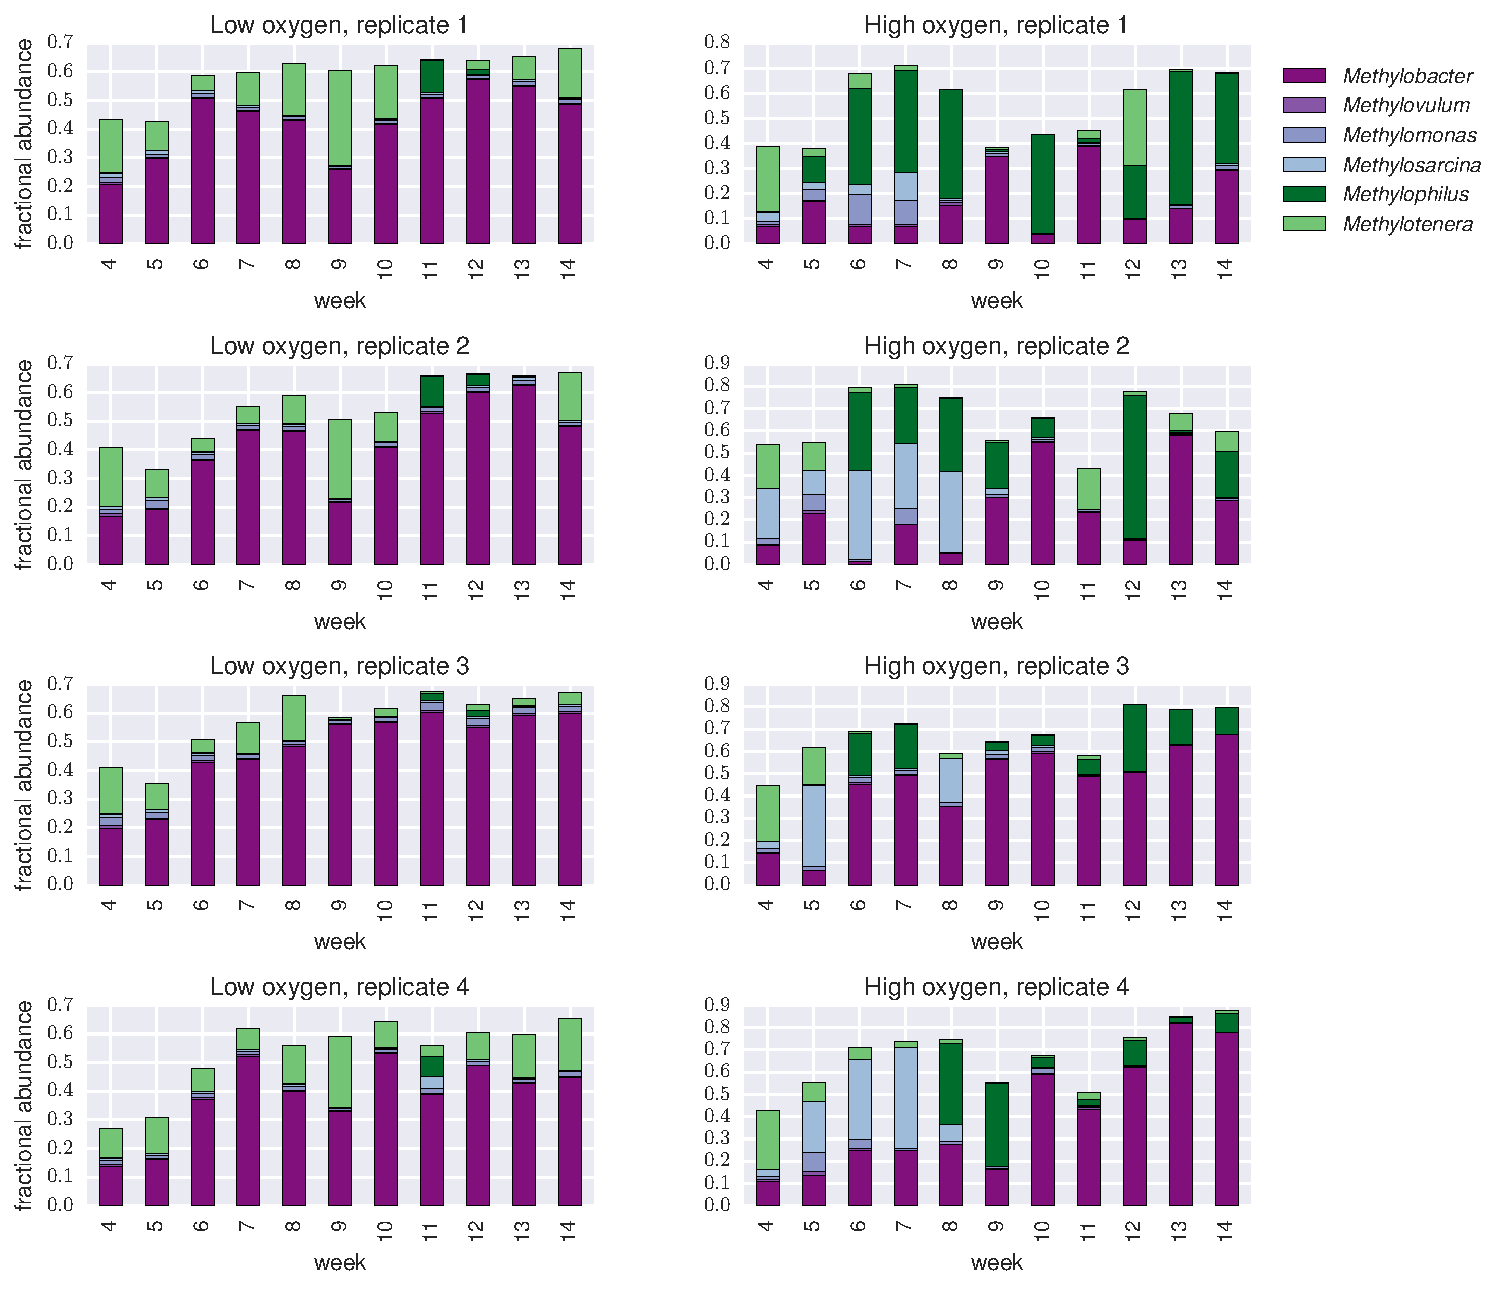
\includegraphics[width=1.0\textwidth]{./tex/chapter2/figures/170313_methanotroph_methylotroph_taxa--portrait.pdf}  % ElvizAnalysis
    \begin{singlespace}
    \caption[Dominant methanotrophic and methylotrophic genera]{
        Fractional abundance of DNA from the dominant methylotrophic genera.
        Purple bars are methanotrophs of order Methylococcales, family \textit{Methylococcaceae}
            (represents major taxa in blue bars of Figure \ref{fig:4dominant_groups}).
        Green bars are non-methanotrophic methylotrophs of order Methylophilales, family \textit{Methylophilaceae}
            (represents major taxa in yellow bars of Figure \ref{fig:4dominant_groups}).
        See Figure \ref{fig:taxonomy} for hierarchical taxonomy reference.
        Vertical gray line indicates the week the oxygen conditions were reversed.
        Like Figure \ref{fig:4dominant_groups}, these bars only reflect reads that mapped to contigs, according to the Elviz pipeline.
        For information about the fraction of reads not assigned to contigs, see Figure \ref{fig:frac_elviz_mapped_to_contigs}.
        }  % Italics are used for bacterial and viral taxa at the level of family and below.  https://wwwnc.cdc.gov/eid/page/scientific-nomenclature
    \label{fig:dominant_genera}
    \end{singlespace}
\end{figure}

\subsubsection{Binning Potential: Elviz Contigs}

%Genomic-scale resolution drove investigation of the potential for sorting these contigs into genome bins.
The goal of this study is a comprehensive description of the samples, ideally in terms of genome bins.
The potential for these Elviz contigs to paint a comprehensive picture of the microbial community was measured by summing all reads assigned to contigs long enough to bin, namely contigs $\geq$ 1.5kb.
Figure \ref{fig:dont_bin_Elviz} shows that while the entire set of contigs represents the samples well, the subset of contigs that are candidates for binning explain less than 20\% of the reads obtained for many low oxygen samples.
Another complication of binning these Elviz contigs, is that binning the contigs for each sample individually would lead to many redundant bins that need to be thinned.
This process is prone to human bias, and can lead researchers to over-fit their bins to their quality measures and thus over-state the quality of their bins.
Nonetheless, if a particular sample is enriched in an organism of interest, use of the contigs from that sample should be conisdered for future binning efforts.


\begin{figure}[H]
\centering
    % /Users/janet/Dropbox/meta4_bins_data_and_files/1703014_is_Elviz-_junk_revised/results
    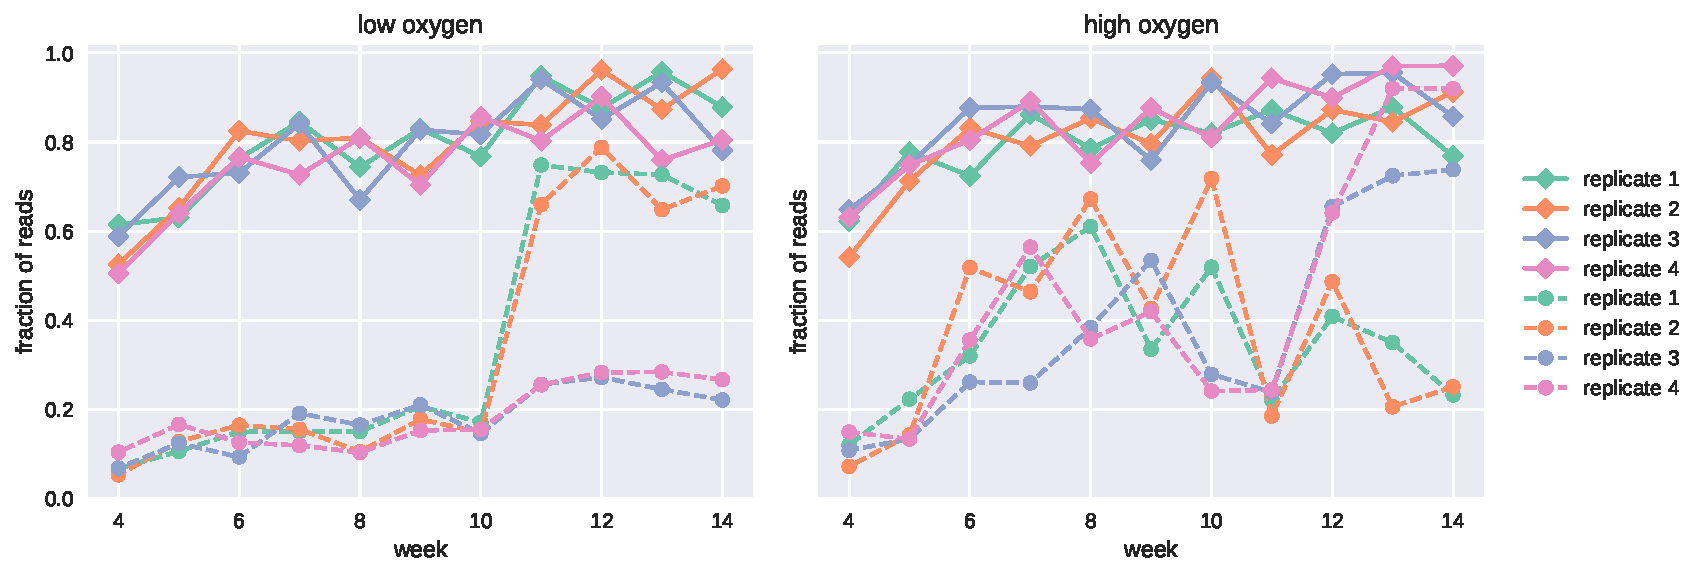
\includegraphics[width=1.0\textwidth]{./tex/chapter2/figures/170314_Elviz_is_not_for_binning--landscape.pdf}  % ElvizAnalysis
    \begin{singlespace}
    \caption[Upper-bound limit on success of binning Elviz contigs]{
        The upper-bound limit on success in binning Elviz contigs, as measured by the fraction of metagenome reads mapped to contigs.
        Lines are colored by replicate.
        Solid lines represent the fraction of reads in the raw \texttt{.fastq} file that map to contigs of any length.
        Dashed lines represent the fraction of reads in the raw \texttt{.fastq} file that map to contigs with length $\geq$ 1.5kb.
        Less than 20\% of the raw fastq reads would be explained by aggressive binning of most low oxygen samples.}
    \label{fig:dont_bin_Elviz}
    \end{singlespace}
\end{figure}

% ----- Map to Isolate Genomes ------
\subsection{Map to Isolate Genomes}

The next simplest approach for identifying which microbes are active in the samples, and what they express is to map the reads to the 55 isolate genomes (listed in Table \ref{table:55genomes}).
The potential efficacy of these results can be measured by quantifying the fraction of metagenomic and metatranscriptomic reads that align to these genomes (recall the pipe diagram, Figure \ref{fig:pipe_leaks}).
Figure \ref{fig:isolate_RNAseq} shows the fraction of the metatranscriptomes that can be explained using these reference genomes.
The low accountability (mostly $<$15\%) guarantees an incomplete portrait of the activity in these samples, so the data was not pursued further.
Despite heroic Lidstrom Lab efforts to isolate strains, the set obtained thus far does not cover the complexity seen in real samples.
This indicates missing taxa and/or dissimilarity between the isolated strains and the ones that dominate in nature.
While this method of describing gene expression was not pursued father, it provides a baseline fraction of RNA mapped for any subsequent metagenomic methods to beat.


\begin{figure}[H]
\centering
    % /Users/janet/Dropbox/thesis/tex/chapter2/figures/170208_fraction_of_transcriptome_reads_mapped_to_isolates.pdf
    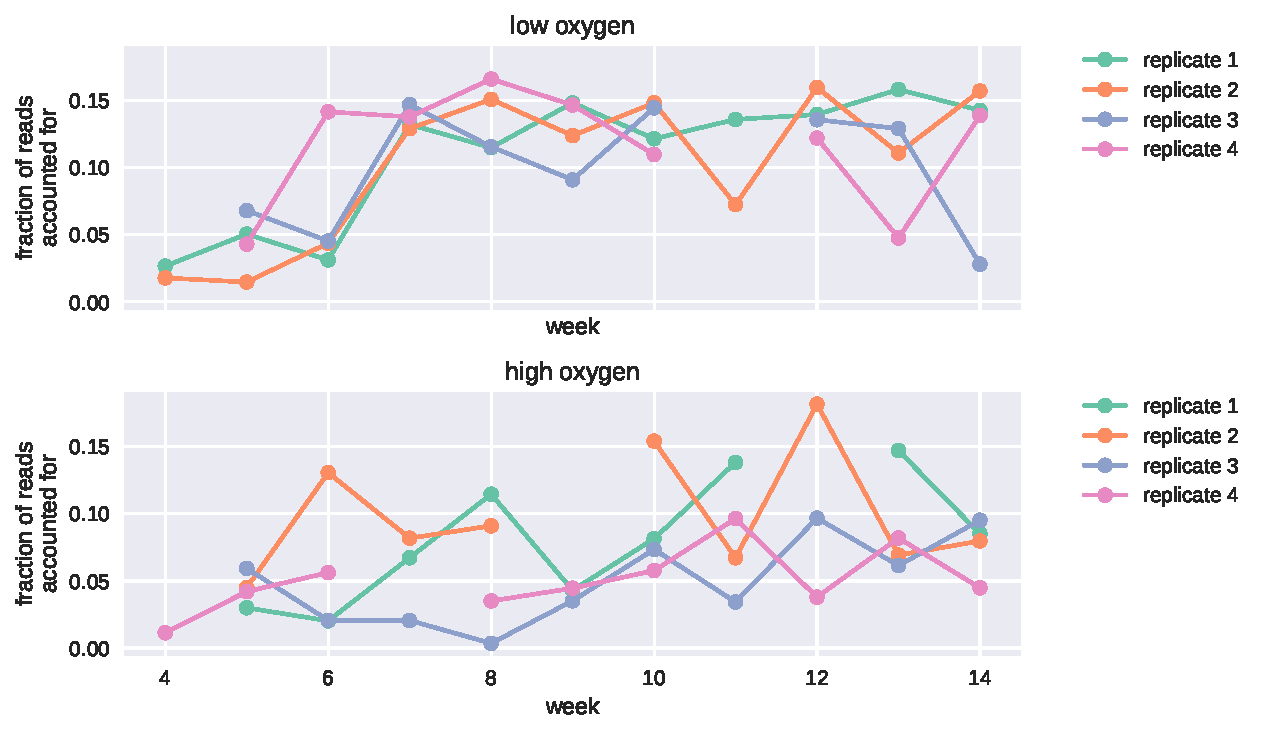
\includegraphics[width=1.0\textwidth]{./tex/chapter2/figures/170208_fraction_of_transcriptome_reads_mapped_to_isolates.pdf}
    \begin{singlespace}
    \caption[Measure of isolate genomes' ability to account for RNA-seq reads]{
        Measure of isolate genomes' ability to account for RNA-seq reads.
        Each dot represents the total fraction of raw reads assigned to genes when mapped to a concatenation of 55 isolate genomes.
        }
    \label{fig:isolate_RNAseq}
    \end{singlespace}
\end{figure}

As noted in the Methods, all computational steps using BWA-MEM and Samtools use default handling of reads that map equally well to multiple places.
This leads to omission of multiply-mapped reads.
Such handling is the best-practice approach for differential abundance analysis, which is the most common workflow for the tools used.
It does, however, lead to under-estimation of gene expression levels and lower accountability of the original fastq reads. % TODO: cite
Higher mapping fractions could be achieved by randomly assigning reads to one target from the set of best potential targets, but this lowers uncertainty about which genes/organisms are most influential in the samples.


% ----- ASSEMBLY ------
\subsection{Assembly}

Given that the Elviz contigs and isolate genomes proved ineffective as reference DNA for comparative analysis of samples, a single set of contigs that could be used to assess all samples was sought.
One workflow for explaining a set of metagenomic/metatranscriptomic samples includes co-assembly of metagenome reads, calling genes on the resulting contigs, mapping the transcriptomes to these contigs, and tabulating the expression levels.
Accordingly, the metagenomes from almost every sample were pooled and assembled into one set of contigs shared by all samples.

Assemblies which produce long contigs are desired, as longer contigs are easier to call genes on and cluster by similarity during binning.
Communities with extremely low complexity (just a few microbes co-existing) can yield long contigs with greater potential for being sorted into high-confidence genome bins. % which are often described by authors as genomes, rather than bins.
As complexity increases, reduced sequencing depth and homologous regions between organisms inhibit the formation of long contigs.
The distribution of contigs obtained (Figure \ref{fig:contig_lengths}) do not suggest a simple community.


\begin{figure}[H]
\centering
    % /Users/janet/Dropbox/meta4_bins_data_and_files/170124_current_metabat_analysis_figures/170123_frac_reads_binned_at_different_contig_lengths_and_total.pdf
    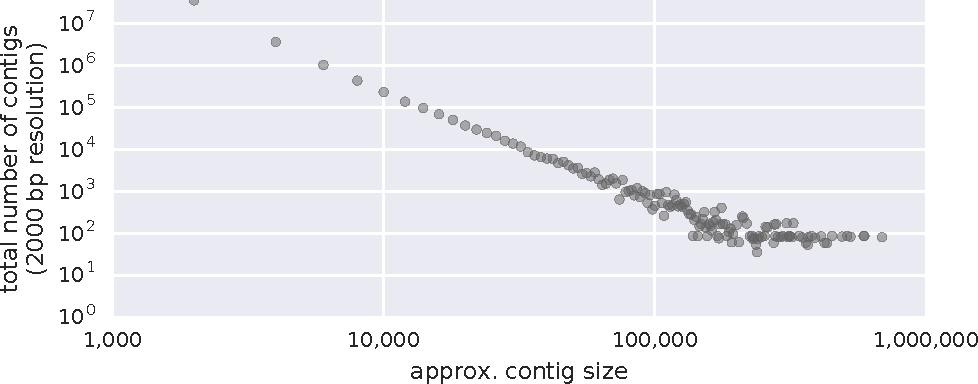
\includegraphics[width=1.0\textwidth]{./tex/chapter2/figures/170123_frac_reads_binned_at_different_contig_lengths_and_total--INKSCAPED.pdf}
    \begin{singlespace}
    \caption[Distribution of contig sizes]{
        Distribution of sizes for contigs assembled by MEGAHIT (2,617,225 contigs in total).}
    \label{fig:contig_lengths}
    \end{singlespace}
\end{figure}



% ----- ANNOTATION ------
\subsection{Annotation}

%[ec2-user@ip-10-0-0-158 map_to_contigs_longer_than_1500bp]$ realpath gene_read_totals.tsv
%/work/rnaseq/alignments/map_to_contigs_longer_than_1500bp/gene_read_totals.tsv
%[ec2-user@ip-10-0-0-158 map_to_contigs_longer_than_1500bp]$ cat gene_read_totals.tsv | wc -l
%107900

%[ec2-user@ip-10-0-0-158 map_to_contigs_longer_than_1500bp]$ realpath map_to_contigs_longer_than_1500bp_genes.tsv
%/work/rnaseq/alignments/map_to_contigs_longer_than_1500bp/map_to_contigs_longer_than_1500bp_genes.tsv
%[ec2-user@ip-10-0-0-158 map_to_contigs_longer_than_1500bp]$ cat map_to_contigs_longer_than_1500bp_genes.tsv | wc -l
%921436  % Includes 5 __ columns, use so 921,431.

Genes were called on contigs with length $\geq$ 1.5kb, in preparation for metatranscriptome studies (Table \ref{table:annotation}).
%Prokka identified 921,431 distinct genes, encoding 107,900 differently named proteins (Table XX).
See supplementary files for the gene \texttt{.fasta} and corresponding \texttt{.gff}. %, and RNA read counts \texttt{.tsv} in each sample.

\begin{table}[H]
\centering
\begin{singlespace}
\caption[Annotation of MEGAHIT contigs]
	{Annotation of MEGAHIT contigs.}
\begin{tabular}{l | c}
 %\toprule
        & statistic  \\
\midrule
	total \# of genes & \texttt{921,431} \\ % /work/jmatsen/170308_assess_Elviz_read_attraction_frac
	number of distinctly name genes & \texttt{107,900} \\
%\bottomrule
\end{tabular}
\label{table:annotation}
\end{singlespace}
\end{table}


% ?? Xox?

%Prokka was able to identify key methanotrophy/methylotrophy genes such as XXX.
%Some proteins were mis-annotated, as is typically observed when using automated annotation tools on methylotrophs.
%For example, many of the glucose dehydrogenases identified are in fact methane monooxygenases, and Xox-MDHs are listed as XXX.


% ?? TODO: make a plot that shows the gene density is lower on short contigs?


% ----- TRANSCRIPTOME ANALYSIS ------
\subsection{Transcriptome Analysis}

% Intro
Mappings of the 88 transcriptomes to the annotated contigs revealed which of the $\approx$0.9 million genes were strongly expressed.
Table \ref{table:top_genes} shows the names of the proteins associated with the highest total of reads mapped, and how many copies of each gene contribute to each sum.
See supplementary files (\texttt{.fasta}, \texttt{.gff}, and \texttt{.tsv}) for per-gene sequences, sequence information, and RNA-seq read counts by sample.

Figure \ref{fig:rna_mapping_bars} shows how well the called genes account for the transcripts seen in the raw sequence data.
The green bars represent a high degree of certainty.
Gray bars correspond to "no feature", which is presumably correlated to short contigs for which gene calls are less likely.
Pink bars are labeled as having low alignment quality, but recall that BWA-MEM sets the quality score to zero when a read maps equally well to two different spots.
It may be possible to improve (shrink) the gray bars via re-assembly of portions of the data (see Section \ref{sect:assembly_discussion}).
Similarly, recovery of reads that map equally well to different places can be brought out of the pink bars if htseq-count's parameters are altered to allow low quality reads to be counted (see Section \ref{sect:multiply_mapped_reads}).
While this alteration would help with describing the big picture of which genes are expressed, it reduces certainty of read mappings and is not appropriate for Chapter \ref{chapter:C}.


\begin{figure}[H]
\centering
    % /Users/janet/Dropbox/meta4_bins_data_and_files/1703016_frac_RNA-seq_mapped/figures/170316_fracs_mapped_unmapped_etc.pdf
    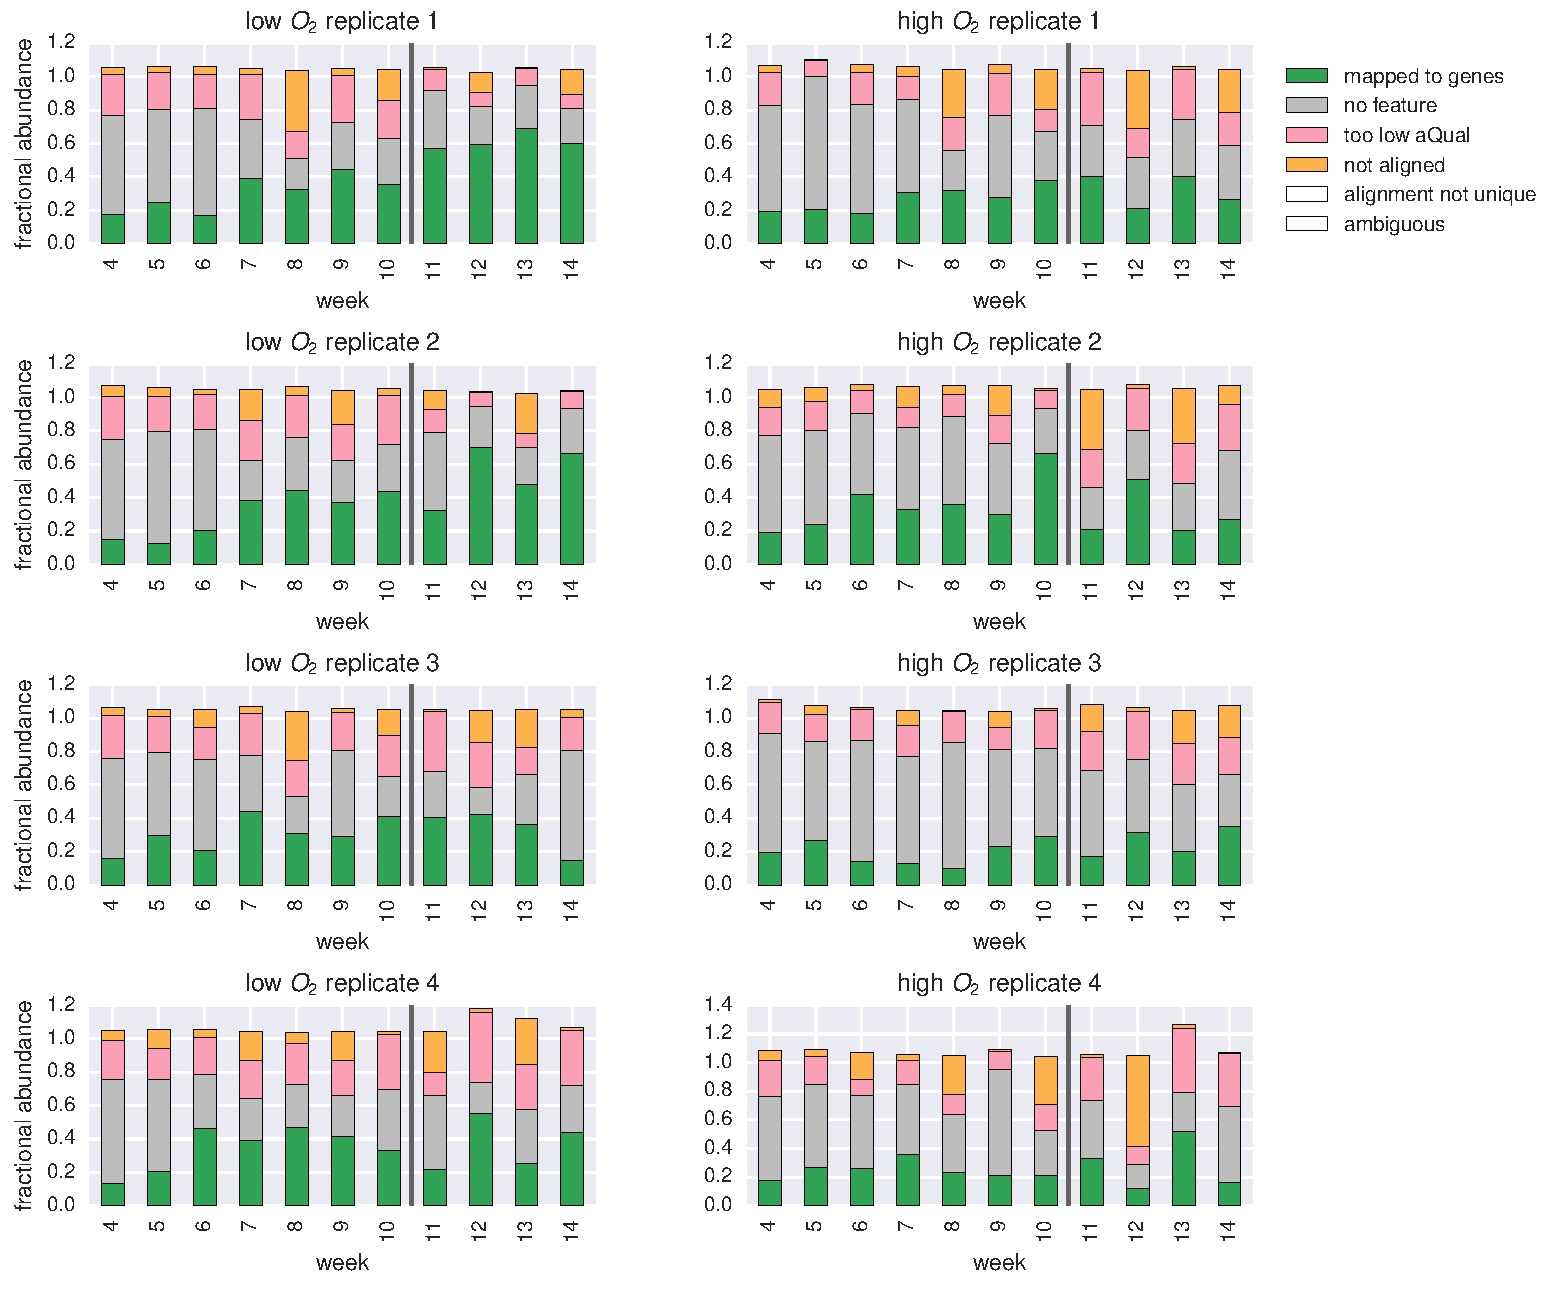
\includegraphics[width=1.0\textwidth]{./tex/chapter2/figures/170316_fracs_mapped_unmapped_etc.pdf}
    \begin{singlespace}
    \caption[Efficacy of mapping RNA-seq to MEGAHIT contigs]{
        Efficacy of mapping RNA-seq to MEGAHIT contigs.
        Bar heights are fractions of reads with respect to the original \texttt{.fastq} files.
        Bar height totals are noticeably greater than one for samples with a larger fraction of reads that map equally well to multiple loci.
        Such multiply mapped reads are included in the pink bar due to being assigned a quality score of zero by BWA-MEM.
        }
    \label{fig:rna_mapping_bars}
    \end{singlespace}
\end{figure}

\subsubsection{Highest Expressed Proteins}
% TODO: add table of highest expressed proteins, and describe.

The top genes include many methanotrophy genes, especially subunits of methane monooxygenase and methanol dehydrogenase (Table \ref{table:top_genes}).
Other highly expressed methylotrophy genes encode products including 3-hexulose-6-phosphate synthase, transketolase, formaldehyde-activating enzyme, and 3-hexulose-6-phosphate isomerase.
The presence of key methanotrophy and methylotrophy genes agrees with the Elviz portrait of methanotroph/methylotroph dominance in every sample.
Other highly expressed genes allow speculation for metabolic roles of other organisms.

Two phage proteins are near the top of the list: Capsid protein (F protein), and Microvirus H protein (pilot protein) (Figures \ref{fig:phage_protein_F}, \ref{fig:phage_pilot_protein}). %
%WTF... Group II intron-encoded protein LtrA ??  http://www.uniprot.org/uniprot/P0A3U0
Phage blooms could contribute to the apparent stochasticity in community rarefaction.
%?? Get isolate stats?? We hoped to beat the benchmark of mapping to the isolates:  median XX %.

Note that Table \ref{table:top_genes} does not include normalization for gene length or sample sequencing depth.
Before dividing by gene length, consistency of gene lengths for loci of the same gene product should be checked.
It is possible that genes encoding product of the same name could be of varying length, depending on how Prokka handles gene fragments.

\subsubsection{Expression of Genes by Locus}

Which copes are expressed, and under which conditions?
Breaking down the expression of these genes by locus and sample reveals which copies dominate.
Many of the patterns appear to be oxygen-dependent, and/or perturbed by the oxygen condition switch for the last four samples.
% TODO: figure of expression.  Include more in appendix.
% FIGURE: pmo subunit A.
For example, the patterns for which \textit{pmoC} locus is expressed in each sample appears to be correlated with the oxygen tension in each sample (Figure \ref{fig:mmo_alpha}).
Exploration of these patterns and analysis of the genes taxonomy can shed light onto how oxygen influences community composition.

\begin{figure}[H]
\centering
    % /Users/janet/Dropbox/thesis/tex/chapter2/figures/170328_loci_read_fracs_Particulate_methane_monooxygenase_alpha_subunit_precursor--portrait--cleaned.pdf
    % /Users/janet/Dropbox/meta4_bins_data_and_files/170328_locus_expression_plots/170328_loci_read_fracs_Particulate_methane_monooxygenase_alpha_subunit_precursor--portrait.pdf
    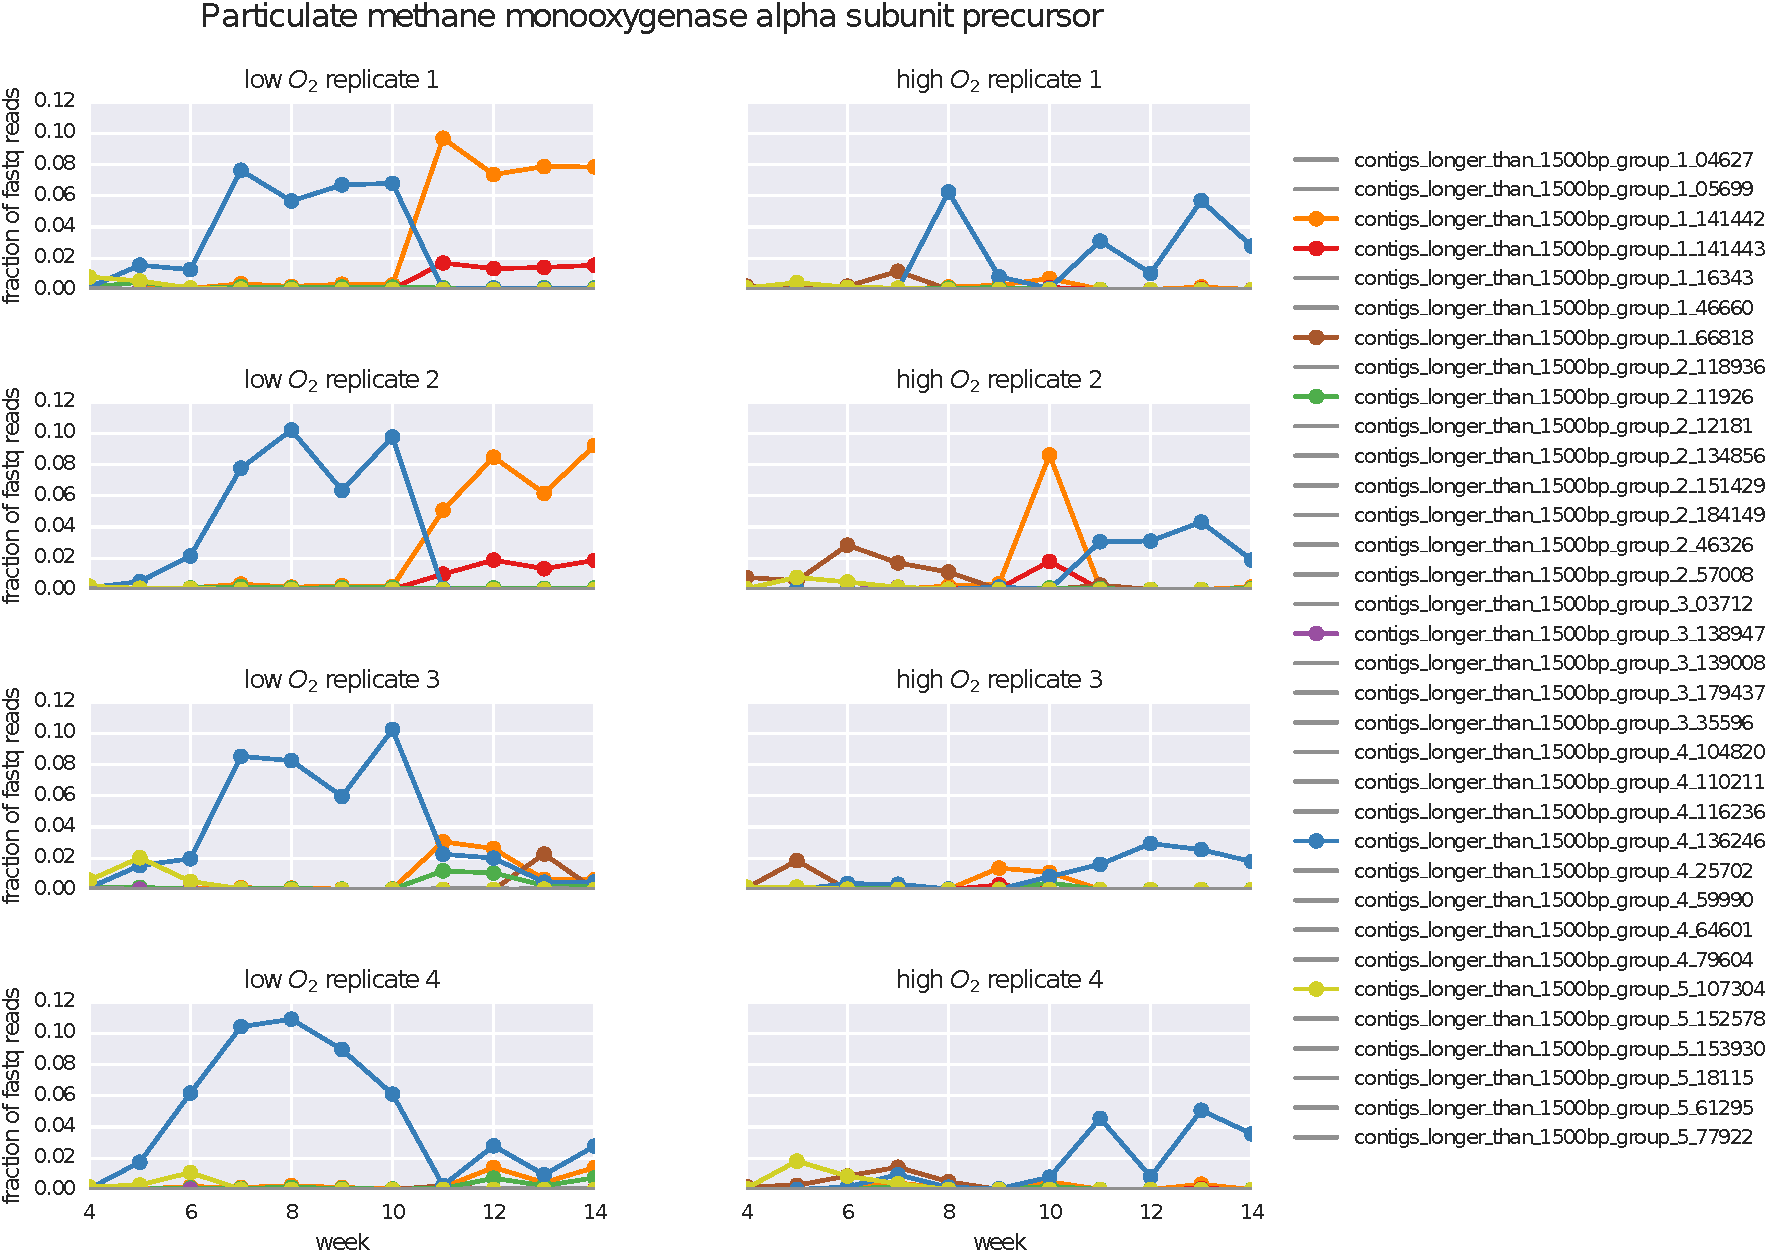
\includegraphics[width=1.0\textwidth]{./tex/chapter2/figures/170328_loci_read_fracs_Particulate_methane_monooxygenase_alpha_subunit_precursor--portrait--cleaned.pdf}
    \begin{singlespace}
    \caption[Methane monoxygenase alpha subunit locus expression profiles by sample]{
        Methane monoxygenase alpha subunit locus expression profiles by sample.
        The legend shows many genes annotated as such, but only the highest expressed loci were plotted with color.
        The gray series have nearly zero expression and thus do not rise above the x-axis.
        }
    \label{fig:mmo_alpha}
    \end{singlespace}
\end{figure}

% ----- BINNING ------
\subsection{Binning of Co-assembled Contigs}

Contigs of length $\geq$ 1.5kb were binned by MetaBAT and MyCC, two leading binning tools.
As mentioned, MyCC does not scale well to large data, so the full dataset including contigs as short as 1.5kb did not complete, even with a high performance AWS instance.

\begin{table}[H]
\centering
\begin{singlespace}
\caption[Binning results: MetaBAT \& MyCC]
	{Binning results: MetaBAT \& MyCC.}
\label{table:sample_read_sizes}
\begin{tabular}{l | cc}
 %\toprule
            & \# bins &  min contig size allowed \\  % consider fraction of contigs binned?
\midrule
	MetaBAT & 330   & 1.5kb \\
	MyCC    & 109   & 2.5kb \\
%[ec2-user@ip-10-0-0-158 metabat]$ realpath .
%/work/m4b_binning/assembly/metabat
%[ec2-user@ip-10-0-0-158 metabat]$ ls bin*.fa | wc -l
%330

%[ec2-user@ip-10-0-0-158 assembly_mycc_2.5kb_56mer_lt_0.4_st_50]$ realpath 20170131_1745_56mer_0.7_cov
%/work/m4b_binning/assembly_mycc_completed/assembly_mycc_2.5kb_56mer_lt_0.4_st_50/20170131_1745_56mer_0.7_cov
%[ec2-user@ip-10-0-0-158 assembly_mycc_2.5kb_56mer_lt_0.4_st_50]$ ls 20170131_1745_56mer_0.7_cov/Cluster*.fasta | wc -l
%109

%\bottomrule
\end{tabular}
\end{singlespace}
\end{table}

%MetaBAT suffers from low binning rates, MyCC suffers from too aggressive of binning.
Figure \ref{fig:binning_frac_reads_mapped} shows this the fraction of the metagenomes that are accounted for by the bins, as a measure of how effectively the bins describe the composition of organisms.
The two sets of lines for the MetaBAT plots measure how well the bins represent the original \texttt{.fastq} files in total (dashed lines), and how well they did using only contigs longer than 2.5kb (to better compare with the MyCC results).

\begin{figure}[H]
\centering
    % /Users/janet/Dropbox/meta4_bins_data_and_files/170201_MyCC_read_accountability_figures/170201_comparable_read_coverage_for_metabat_and_mycc_3kb.pdf
    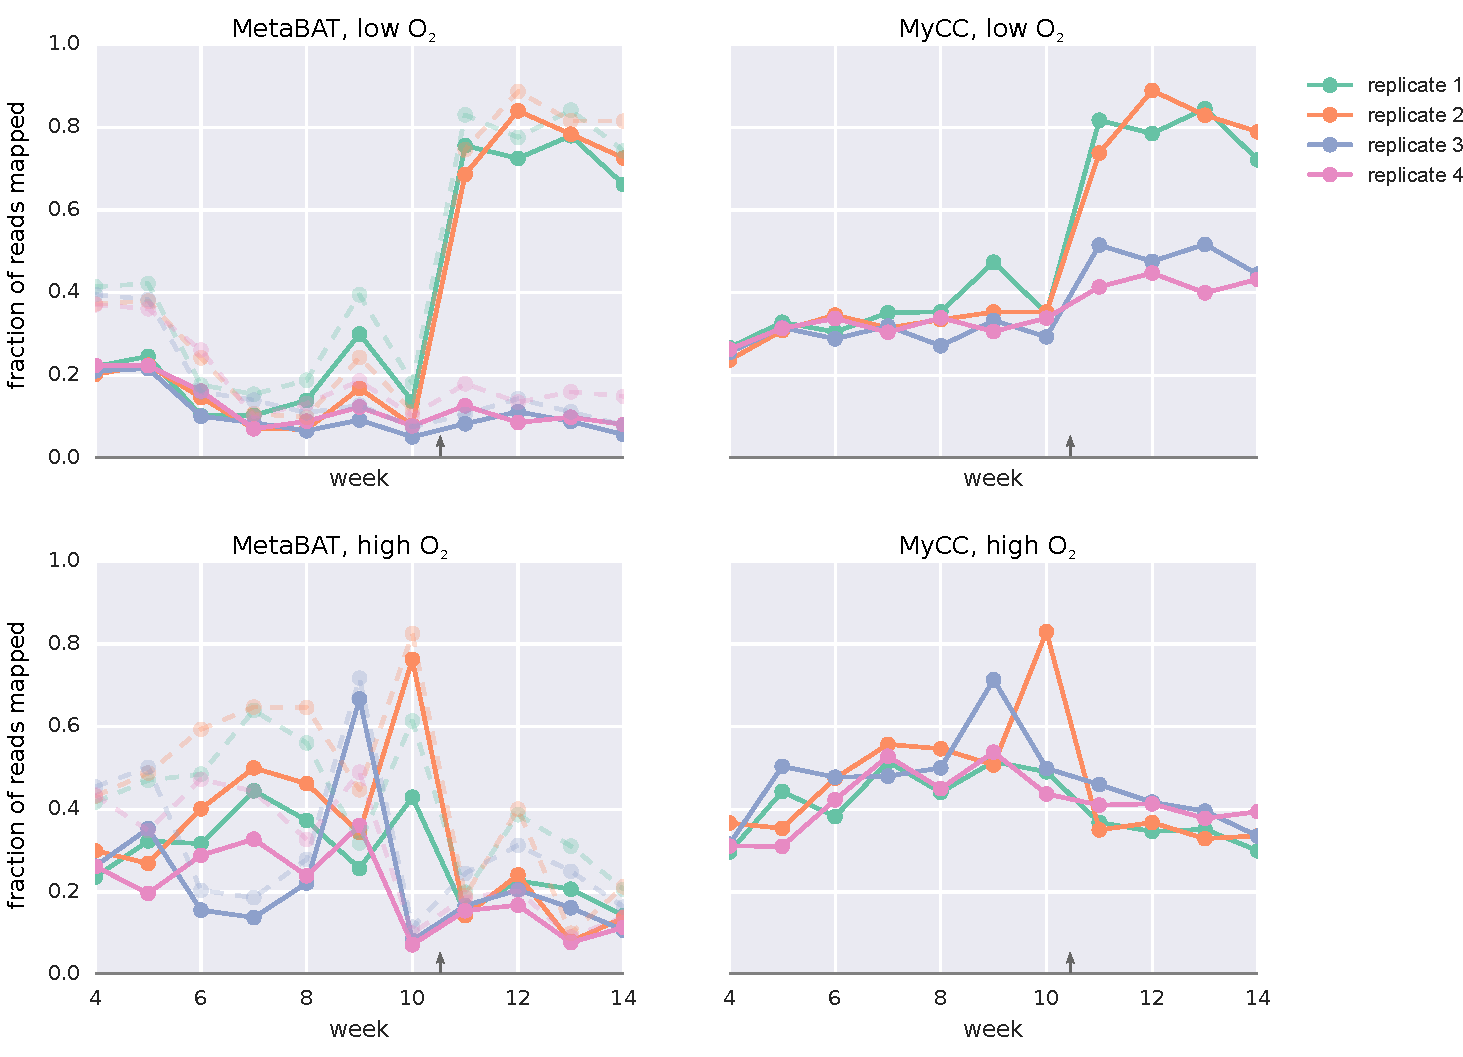
\includegraphics[width=1.0\textwidth]{./tex/chapter2/figures/170201_comparable_read_coverage_for_metabat_and_mycc_3kb--INKSCAPED.pdf}
    \begin{singlespace}
    \caption[Fraction of reads accounted for by MetaBAT and MyCC bins]{
        Fraction of reads accounted for by bins generated via MetaBAT (min contig size = 1.5kb, default settings) and MyCC (min contig size = 2.5kb, settings adjusted for memory issues).
        Points represent the fraction of reads that are associated with binned contigs for each sample.
        The solid MetaBAT lines represent the fraction of reads associated with contigs of length $\geq$ 2.5kb, as an appropriate comparison to the MyCC run.
        The dashed MetaBAT lines represent the full fraction of reads accounted for by the actual MetaBAT bins, which include contigs as short as 1.5kb.
        The arrows after week 10 in each plot indicate that all subsequent samples were treated with the opposite oxygen tension as the label indicates.
    }
    \label{fig:binning_frac_reads_mapped}
    \end{singlespace}
\end{figure}

MetaBAT with default settings produced bins with low sample accountability, whereas the MyCC bins represented a high fraction of the raw sample reads.
This represents a trade-off between precision and recall, a balance inherent to binning regardless of the tool used.

% MetaBAT comments
One striking trend in the MetaBAT results is the difference in read accountability between replicates 1/2 and 3/4 at the low oxygen state. %in the fraction of reads associated with binned contigs between low oxygen replicates 1/2 and 3/4.
The large difference is associated with the proportion of reads associated with long contigs (Supplemental Figure \ref{fig:contig_dist}).
The poorly represented samples are biased more toward short contigs.
While noting that the last 4 data points in each series have the opposite oxygen condition as the series label, see that the high oxygen samples in all four subplots are better reflected by MetaBAT bins.
This source of this conundrum has not yet been resolved, but could be due to a smear of organisms for which assembly performed poorly.
The Elviz data points towards the genus \textit{Methylobacter}, given its dominance in samples at the low-oxygen state.
BLAST or other computational tools could be used to identify the taxonomy of contigs that are not binning well. %identify the taxa for the contigs which are binning well, though high-throughput techniques would be prudent given the number of contigs.

Figure \ref{fig:mycc_binned_more_contigs} also shows MyCC's increased efficacy at representing the raw sequencing reads.
Upon further investigation, it was revealed that MyCC binned $>$99\% of all contigs supplied, including the shorter ($\approx$ 2.5kb) contigs which carry greater uncertainty. %(Figure \ref{fig:mycc_binned_more_contigs}).
Aggressive binning is associated with low specificity, meaning inclusion of contigs that do not belong in bins. %binning of contigs that do not belong with the others in the bin.

\begin{figure}[H]
\centering
    % /Users/janet/Dropbox/meta4_bins_data_and_files/170202_comparing_MyCC_to_metabat/170206_improved_fracs_of_contigs_binned_by_MyCC.pdf
    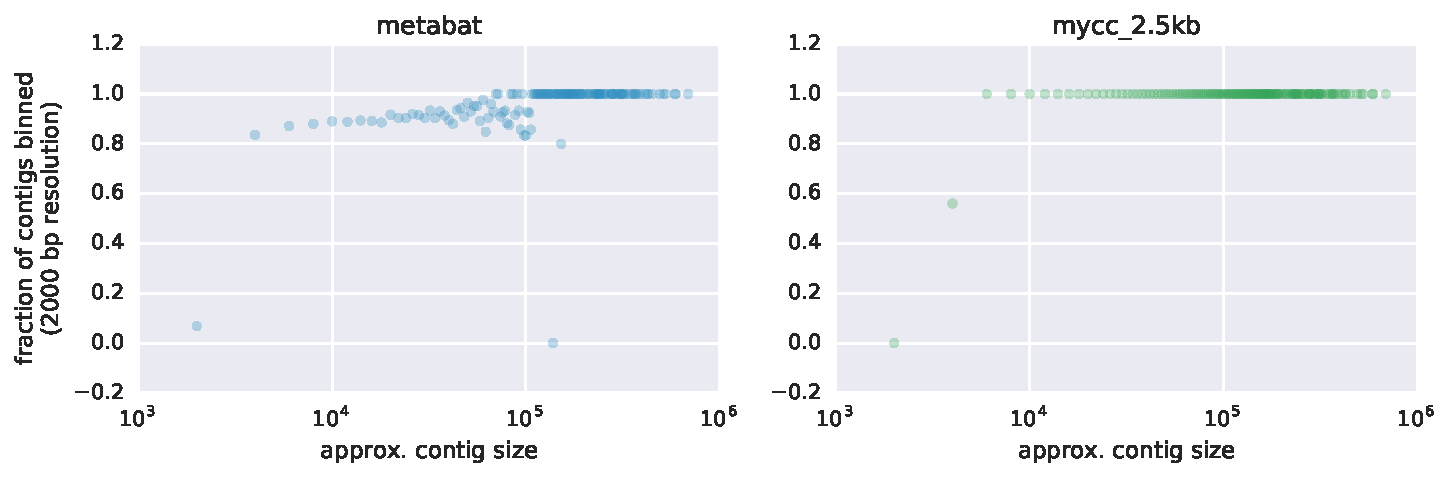
\includegraphics[width=1.0\textwidth]{./tex/chapter2/figures/170206_improved_fracs_of_contigs_binned_by_MyCC.pdf}
    \begin{singlespace}
    \caption[MyCC binned contigs more aggressively than MetaBAT]{
        MyCC binned contigs more aggressively than MetaBAT.
        With the settings used, MyCC binned $>$ 99\% of contigs at all lengths. %, for all lengths.
        The one MyCC dot near y=0.6 had a $>99\%$ binning rate as well, but is lower because the point includes contigs that were ineligible for binning (lengths below the 2.5kb cutoff).
        }
    \label{fig:mycc_binned_more_contigs}
    \end{singlespace}
\end{figure}

Figure \ref{fig:mycc_contamination} reveals the consequence of the aggressive MyCC binning: high contamination scores according to CheckM.
To test CheckM's predictive accuracy on methylotrophic genome bins, a positive control test was used: CheckM was applied to the 55 genomes used in the isolate studies.
While the marker lineages used were often surprising (e.g. Rhizobiales, Actinomycetales), the completeness and contamination statistics CheckM returned for these positive controls were nearly perfect (Table \ref{tab:checkm_isolate}).
Thus future binning efforts should aim for nearly 100\% completeness and less than a few percent contamination, even when CheckM uses the default (non-methylotrophic) marker lineages.
High measures of strain heterogeneity may be tolerated, as some of these isolates were estimated as having 100\% strain heterogeneity  (Table \ref{tab:checkm_isolate}).
% high sensitivity, low specificity.

Given the small fraction of the metagenome reads explained by MetaBAT (Figure \ref{fig:mycc_contamination}), and high contamination scores of the MyCC bins (Figure \ref{fig:mycc_contamination}), binning has been placed on hold.
See Section \ref{chA_future_steps} below for suggested next steps in the binning workflow.


\begin{figure}[H]
\centering
    % /Users/janet/Dropbox/meta4_bins_data_and_files/170202_comparing_MyCC_to_metabat/170202_MyCC_has_higher_contamination.pdf
    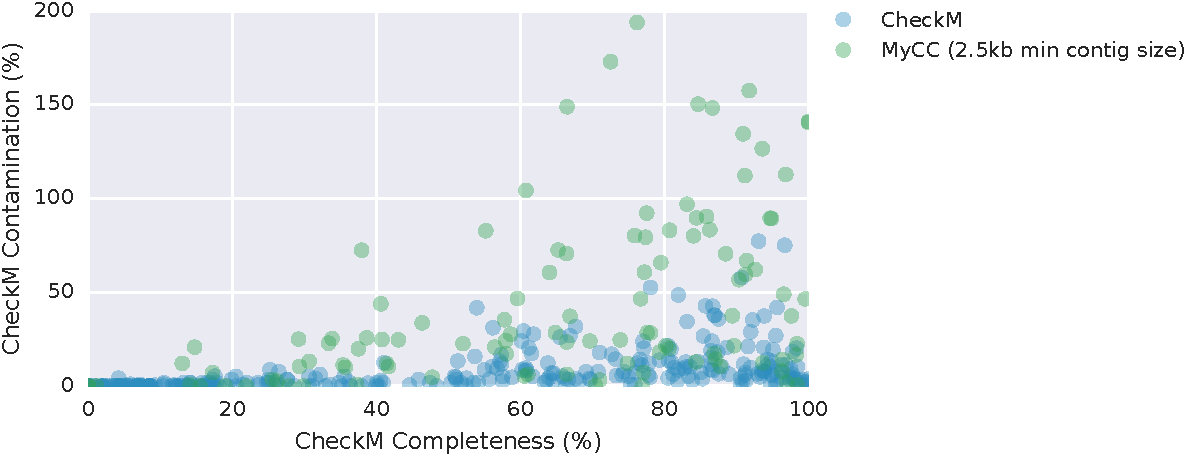
\includegraphics[width=1.0\textwidth]{./tex/chapter2/figures/170202_MyCC_has_higher_contamination--cleaned.pdf}
    \begin{singlespace}
    \caption[MyCC bins have higher contamination scores than MetaBAT bins]{
        MyCC bins have higher contamination scores than MetaBAT bins.}
    \label{fig:mycc_contamination}
    \end{singlespace}
\end{figure}

% ----- BIN TAXONOMY ------
\subsection{Bin Taxonomy}

Once final bins are in hand, taxonomic labels need to be assigned.
This can be done by aggregating information from several sources, including the CheckM marker gene set (coarse label), PhyloPhlAn results (maximally specific), and average nucleotide identity (ANI, below).

PhyloPhlAn was applied to the MetaBAT bins, producing taxonomic labels that did not agree particularly well with the CheckM labels.
This adds motivation for revisiting binning before describing the broad community composition in terms of genome bins.
% TODO: show data on this?  Put in Appendix?

% ----- ANI ------
\subsection{Average Nucleotide Identity (ANI)}

Average nucleotide identity (ANI) can also contribute evidence for taxonomic assignments, especially in cases such as this project when there are many environmental isolates from the exact ecosystem to use as references.
The JGI ANI tool was used on all pairs of MetaBAT bins and isolate genomes, producing a large matrix of ANI values, a subset of which is shown in Figure \ref{fig:ANIs}.

\begin{figure}[H]
\centering
    % /Users/janet/Dropbox/thesis/tex/chapter2/figures/170123_frac_reads_binned_at_different_contig_lengths_and_total--INKSCAPED.pdf
    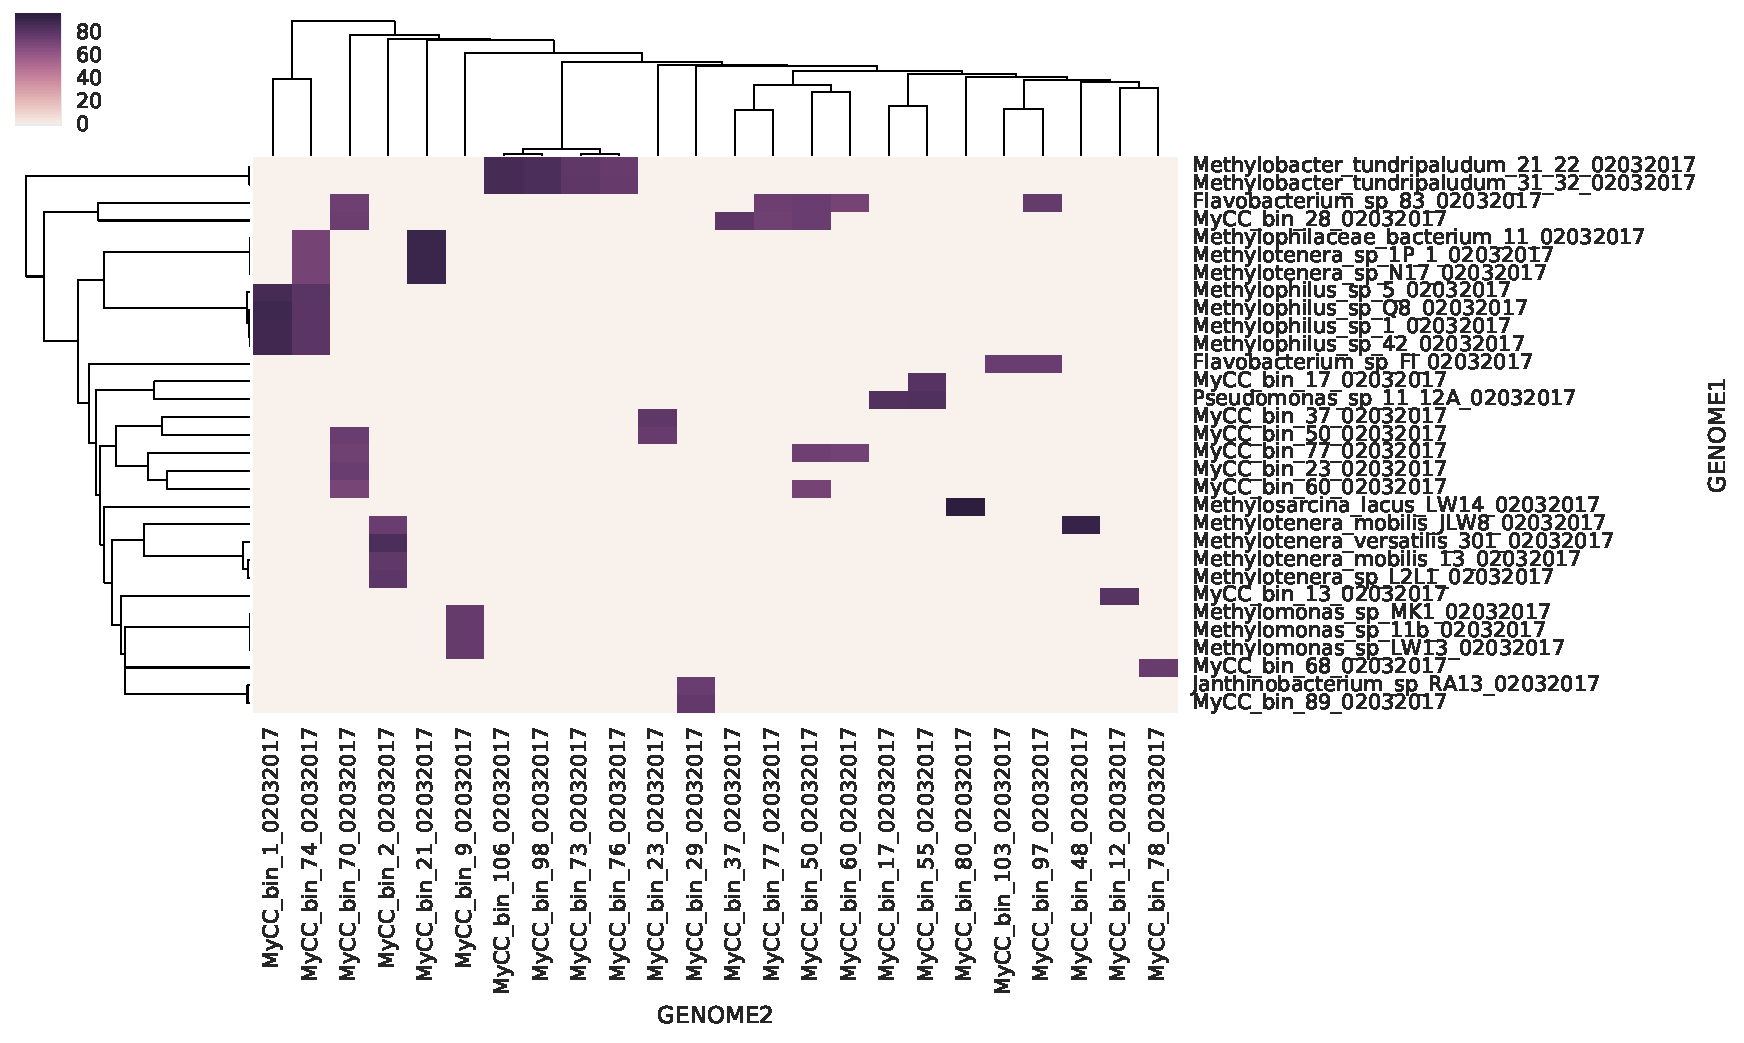
\includegraphics[width=1.0\textwidth]{./tex/chapter2/figures/170203_demo_of_ANI_heatmap.pdf}
    \begin{singlespace}
    \caption[Demo use of ANI to infer taxonomy of genome bins]{
        Demo use of ANI to infer taxonomy of genome bins.
        ANIs between all pairs of bins, and all isolate/bin pairs was computed, tabulated, and plotted to identify taxonomy of genome bins.
        This strategy, in conjunction with taxonomy calls by PhyloPhlAn \cite{segata2013} are recommended for taxonomic assignments when the final bins are identified.
        This clustermap was produced from raw ANI statistics via Seaborn (\url{https://github.com/mwaskom/seaborn}).}
    \label{fig:ANIs}
    \end{singlespace}
\end{figure}

% ------ FUTURE STEPS
\section{Future Steps}
\label{chA_future_steps}


%Big picture
This analysis aimed to describe a wholistic picture of the microbes in the mixtures, and assess how gene expression supports methane oxidation.
This thesis identified the key trends, but more precise understanding can be gained by diving deeper into many of the topics described.
Insights gained by iterating through pipeline steps have revealed possibilities to improving the analysis by modifying each step, as described in the following sections.

% ----- General NEXT STEPS ------
\subsection{Goal Setting for Future Directions}

This thesis highlights the challenge of information loss at each step of the analysis pipeline (recall the pipeline analogy in Figure \ref{fig:pipe_leaks}).
Give that the current goals are to describe broad trends of microbial abundance and activity, setting specific goals for information retention in future work is essential.
For example, substantial information in the metagenome \texttt{.fastq} files was lost along the path from raw reads to binned contigs.
Before future binning work is done, measurement of the upper-bound of binning success should be measured.
Specifically, the upper bound for the fraction of the metagenome and metatranscriptome reads that can be explained by metagenome bins can be calculated by counting all reads that align to contigs longer than 1.5kb, as was done in Figure \ref{fig:frac_elviz_mapped_to_contigs} for the Elviz Contigs.
If the fraction of reads mapping to these longer contigs is not sufficient for future publication, assembly should be re-visited (see below), or goals should be readjusted.

% TODO: insert figure of upper-bound for binning potential of these metagenomes.

% ----- Multiply Mapped Reads: NEXT STEPS ------
\subsection{Investigate Multiply Mapped Reads}
\label{sect:multiply_mapped_reads}

If the aim is to describe the community composition and gene expression broadly, investigation of multiply mapped reads is key.
As mentioned, BWA-MEM flags reads that map equally well to two loci as having a quality score of zero.
This means that any gene that appears twice in the reference contigs will have zero reads mapped to it.
Similarly, two homologous genes that attract a similar set of reads will have under-estimated gene expression.

This loss of multiply mapped reads is expected to be a problem for highly conserved genes such as particulate methane monooxygenase (pMMO).
Estimations of methanotroph abundances that rely on counting reads that map to various pMMO copies should have large associated uncertainty values.
One possible way to handle these data is to have three statistics associated with read counts for each gene.
The classically reported BWA-MEM read count will be preserved, but a second column could represent the number of additional reads that could be assigned to a gene if multiply mapped reads were spread evenly across their potential reference targets.
To give that number context, it would be beneficial to have a third column informing how many genes were similar enough to have caused read mapping ambiguity.

% ----- ASSEMBLY NEXT STEPS ------
\subsection{Assembly: Next Steps}
\label{sect:assembly_discussion}

Like all steps of metagenomics, assembly in itself is an art.
There is not one best assembly per data set, as two different research goals could lead to two different ideal assemblies.
For this thesis, the goal was a wholistic portrait of which organisms are present in natural communities.
While the assembly used throughout this chapter was appropriate for that question, there is potential to use additional assemblies to target particular organisms of interest.

%Re-assemble to find rare ones
New assemblies could be done with the aim of making contigs that bin a particular organism well.
The enumerations of the taxa present in each sample, the gene expression profiles, and trends across samples will be explored to identify uncultivated taxa to target.
For example, it is hypothesized that there is a "smear" of similar uncultivated \textit{Methylobacter} strains in these samples.
If genes thought to be associated with different \textit{Methylobacter} strains are found in particular samples, those could be re-assembled separately to get longer \textit{Methylobacter} contigs and thus better bins.
Another possibility is to iteratively bin, remove reads that map to those bins, and re-assemble the leftovers.
These approaches may also lead to bins of important non-methylotrophs, whose metabolic role is least understood.

%This is a computationally expensive and likely laborious path to wholistic community descriptions, but is possible.

% ----- BINNING NEXT STEPS ------
\subsection{Binning: Next Steps}

The analysis shown in this chapter highlights great opportunity to improve the bins and potentially allow for wholistic descriptions of the communities.
The easiest first step is to iteratively test MetaBAT's performance with different binning parameters as the authors suggest.
The resulting bins can be assessed, again by (a) CheckM completeness and contamination scores, (b) fraction of metagenomes that are attracted to bins, and (c) the fraction of transcriptomes that are attracted to them.
Special care can be taken to bin \textit{Methylobacter} strains.

In addition, there are many tools which have not yet been tried.
One promising tool from the Banfield Lab \cite{sieber2017}\footnote{\url{http://biorxiv.org/content/early/2017/02/11/107789}} just appeared on the Biology preprint server, bioRxiv.
This tool uses an ensemble of binning algorithms (MetaBAT\cite{metabat2015}, MaxBin \cite{wu2015}, CONCOCT \cite{concoct2014} and tetraESOMs \cite{dick2009}).
It counts the number of single-copy marker genes in candidate bins, removes good looking bins, and re-bins the remaining contigs.
Given the broad efficacy of ensemble methods in machine learning, exploration of this tool is highly recommended.



% ----- BIOLOGY NEXT STEPS ------
\subsection{Biology: Next Steps}

The dataset prepared in this analysis allows investigation of many biological questions.
Many of these questions are best answered with genome bins.
For example, one topic of excitement in the field of methylotrophy pertains to two alternative methanol dehydrogenase systems.
Recently it has been discovered that some organisms prefer to use lanthanum-dependent \textit{xox} methanol dehydrogenases, rather than the classically studied \textit{mdh} methanol dehydrogenases. %TODO: cite
Though lanthanum was not intentionally supplied to the organisms in this study, it is possible that lanthanum was present in trace amounts.
Identification of expression levels of these two methanol dehydrogenase alternatives in these samples will be explored soon.

Not all questions, however, require genome bins.
Building taxonomic trees of the various signature genes such as methane monooxygenase can give higher resolution insight into community composition inferred in Figures \ref{fig:4dominant_groups}, \ref{fig:dominant_genera}.
There is also potential to explore signatures of phage in the existing contigs.


% ------ CONCLUSIONS
\section{Conclusions}

In conclusion, this 88-metagenome, 88-metatranscriptome data set was designed to allow identification of dominant taxa and gene expression in a natural methane oxidizing microbial community.
The Elviz data was aggregated on taxonomic label to illustrate the fractions of the metagenomes attributed to different taxa (see Figures \ref{fig:4dominant_groups}, \ref{fig:dominant_genera}).
These data were not appropriate for comparison across samples, or assembly into contigs, so an assembly was done with nearly all of the metagenomes.
These contigs were binned into a draft set of bins, which highlighted the challenge of getting enough good bins to illustrate an entire population's dynamics.
% TODO: suggest quality checks so we know how good the set is.
% TODO: note dominant taxa

The contigs were annotated and the genetic content was explored.
In total, 921,431 million genes were identified, encoding 107,900 different proteins.
Oxygen-dependent trends in locus expression were identified, supporting evidence that oxygen is an important and only somewhat understood factor in community composition and function.

The biology inferred in this preliminary round of studies drove new ideas for iterating through the pipeline again, with new goals and refinement strategies in mind.
While the community structure may be too complex for current binning tools to explain without extensive manual labor, targeting particular taxa for binning will allow observation of community dynamics for the major players.
In addition, the ability to extract more information about community structure and dynamics is explored in Chapter \ref{chapter:C}.




 % ========== Chapter 3

%\chapter{Machine Learning for Metagenomics and Metatranscriptomics}
%\label{chapter:C}

\section{Abstract}

The potential to apply statistical/machine learning for metatranscriptomics data is explored, using the data of Chapter \ref{chapter:B}.
These data ($N$  = 88 samples, $d$ = 0.9 million measurements per sample) are too large to capture more than simple trends via manual inspections as is done in Chapter \ref{chapter:B}.
While typical machine learning datasets have much larger sample sizes ($N$), select regularized statistical learning techniques are promising.
This chapter focuses on two of them: canonical correlation analysis (CCA), and exploration of the approximated gene-expression partial correlation (pcor) matrix.
Results generated from this chapter are intended to generate hypotheses that will be tested with wet-lab experiments.
This chapter is left at an exploratory level; subsequent students will pursue the identified methods.


% ===========================
% ===== INTRODUCTION ========
% ===========================
\section{Introduction}

\subsection{Machine Learning for Metatranscriptomics}

\subsubsection{Essential Vocabulary}

Before jumping in, this subsection describes key vocabulary for statistical/machine learning.
"Sample" is used equivalently to biology, and the variable $N$ is used to denote the sample size.
In this experiment, $N$=88 for the 88 bottles that were sequenced.
"Feature" describes a measured value that is supplied to an algorithm.
A feature could be a raw measurement value (e.g. expression of gene A), or potentially some abstracted version of one or more measurements (e.g. $log$(expression), or (expression of A)*(expression of B).
The variable $d$ describes the number of features for each sample.

Machine learning is often used to make predictions, so there are terms to describe the different datasets used to train, validate, and test the models.
Ideally a new dataset is split into training data, and test data.
Training data are usually further split into chunks which can be iterated over to tune model "hyperparameters", a process called "cross-validation".
One example of a hyperparameter is the "regularization" strength, a measure of the penalty on large coefficients in models. % (discussed in Section XX).
These techniques allow tuning and evaluation of the model without compromising future predictive accuracy.

\subsubsection{Considerations for Meta-omics Data}

%Intro
The learning techniques chosen for this chapter were highly influenced by the properties of the underlying data.
These properties include sample independence, the samples size, compositional dependency, noise, high-dimensionality, and sparsity.
Each is described to contextualize model selection and analysis, and to aid in future consideration of other statistical frameworks.

\subsubsection{Non i.i.d. Sampling}
Machine learning techniques are generally applied to large datasets, where each data point is assumed to be independent and sampled from an identical data-generating processes (i.i.d.).
For example, a die that is more likely to roll a 6 if a 6 was just rolled exemplifies a violation of i.i.d.
Another violation example is a die that is more likely to roll a 6 when it is warm in the room.
The time-series nature and differences in \ce{O2} are analogous violations of i.i.d. assumptions for this dataset.
This i.i.d. violation can be beneficial, if perturbations allow more signal in the measurements, but can compromise generalizability.
Specifically, i.i.d. violations are more likely to produce models that are over-fit to the particular sample set and less likely to generalize to new data.
The concern about i.i.d. violations is set aside for this chapter given that wet-lab experiments will be designed to verify promising results.

\subsubsection{Sample size}
Machine learning is typically applied to datasets with sample sizes in the thousands or millions.
Some classic example domains include prediction of housing prices, or recognition of hand-written digits \cite{friedman2001}.
Access to tens of thousands of sample points allows the underlying structure to be discovered despite noisy measurements.
The data in this study have small $N$, limiting the number of frameworks that are appropriate.
In particular, this small $N$ is not suitable for generating predictive models.

In machine learning, predictive accuracy is tested by applying a model to un-seen data, and assessing the quality of the predictions.
Thus, one must have enough data to set aside test data that is never touched until the model is to be published.
The importance of not touching these test data until the model is published can not be over stated.
Assessing model accuracy on the test set before model development is complete often leads to over-fitting to the training data because the researcher will make subsequent modeling choices with those fit statistics in mind.
Given an $N$ of only 88, predictive models cannot be produced.
This is again consistent with the intention of this chapter to only use results for hypothesis generation.

\subsubsection{Compositional}
A further challenge of this dataset is that metagenomics and metatranscriptomics data are fundamentally compositional in nature: counts are sampled from a pool and absolute measures are not available \cite{tsilimigras2016, aitchison1982}.
As an illustration of the concern about compositional data, consider a hypothetical sample having only two genes: A and B.
Let genes A and B each have 1 unit of expression in a sample.
Then sampling of 60 reads leads (on average) to 30 reads counted per gene.
Now consider a second sample where B's expression is doubled but that of A remains constant.  When 60 reads are sampled again, only 20 will be associated with A and 40 will now be associated with B.
It thus appears that A's expression level has decreased when in fact only B's expression increased.
In the two-gene example above, the compositional effect is severe, however, as the number of expressed genes increases, the compositional effect grows less strong.

When multiple organisms are present, equivalent compositional effects occur across species.
Fluctuations in the abundance of one dominant organism can produce significant correlations for genes belonging to other microbial pairs that would be absent if comparing absolute measures of gene expression levels.
As with the example above, these cross-species compositional effects diminish as the number of abundant organisms increases.
In the limit of large community complexity, the compositional nature of metatranscriptomics/metagenomics data can be neglected \cite{tsilimigras2016}.
This thesis assumes that the diversity of abundant organisms and number of expressed genes is high enough to find real biological signal above the effects of compositional artifacts.

\subsubsection{Noise}
Consideration of experimental noise is necessary for analysis of metagenomics/metatranscriptomics data, as there are many noise-generating steps.
The first source of noise is biological variation.
Different samples have different population evolution trajectories.
These are often driven by unknown latent variables, and thus cannot be controlled for.
There is also noise that is common to all sequencing datasets, such as amplification biases, sequencing biases, etc..

Additional layers of noise are added when inferring the origin of these reads.
The reference DNA to which reads are mapped is known to be imperfect (see Figures \ref{fig:4dominant_groups}, \ref{fig:rna_mapping_bars}), so the tabulated RNA-seq measurements carry uncertainty.
On top of that, there is ambiguity in how to count reads that map equally well to two or more places \ref{sect:multipli_mapped_reads}).
This chapter explores the potential of finding signal in spite of these unavoidable layers of noise.

\subsubsection{High Dimensionality}
%Example of over-fitting
High dimensionality relative to the sample size can lead to over-fit models if model complexity is not limited \cite{friedman2001}. % pg 38: bias variance trade-off.
For example, consider a housing price dataset with $N$=100 houses, and $d$=1,000 measurements including some presumably uninformative measurements such as the number of steps to the front door, and the last digit of street address.
If only ten variables are allowed in the model, fitting is likely to select the most influential variables (e.g. square footage).
However, if an arbitrarily large model is allowed, the model is likely to include the nonsense features.
Thus it is essential to limit model complexity when $d$ is larger than N.
Regularization is a common technique that adds an additional term to the objective function which penalizes large coefficients \cite{friedman2001}.
Regularization strategies are discussed below, and featured in all techniques highlighted in this chapter.

\subsubsection{Sparsity \& Heavy-tails}
%Sparsity
Many of the metatranscriptomics read count measurements for the 0.9 million genes are zero, indicating high sparsity.
For the 754,836 genes found to have nonzero expression in at least one sample, only 10.6\% of read count values are nonzero.
    % 0.10595531527859875.  See np.count_nonzero(read_counts, axis=1)/elements*1.0 in /misc 170403_iid_and_non-gaussian_figures
To illustrate, Figure \ref{fig:sparse_RNA-seq} shows the read counts for 150 randomly selected genes (columns) across samples(rows).
White rectangles indicate zeros.  All nonzero values are highlighted in color.
Many algorithms are not designed to handle this level of sparsity.
For example, models that use Gaussian (normal) distributions to represent the underlying data should not be assumed to handle sparsity, unless explicitly stated.

%Heavy-tailed distributions
The distributions of counts are also heavy-tailed: large read counts are less common than small counts.
Sparsity aside, these tails are problematic for many model classes, including those based on Gaussian distributions.
%The majority of methods explored in this chapter transform the raw distribution, or statistics derived from them.
The models selected in this chapter are reasonable choices given the sparsity and heavy tails, though even stronger adaptations of these models for high sparsity are likely available in the statistics literature if subsequent students are open to programming their own algorithms.


%\subsection{Canonical Correlation Analysis of Metagenomic Gene Expression}

\begin{figure}[H]
\centering
    % Original: /Users/janet/Documents/Lidstrom Lab Work/meta4_bins_data_and_files/170403_sparsity_and_heavy_tails/20170403_sparsity_illustration--754836_nonzero_features.pdf
    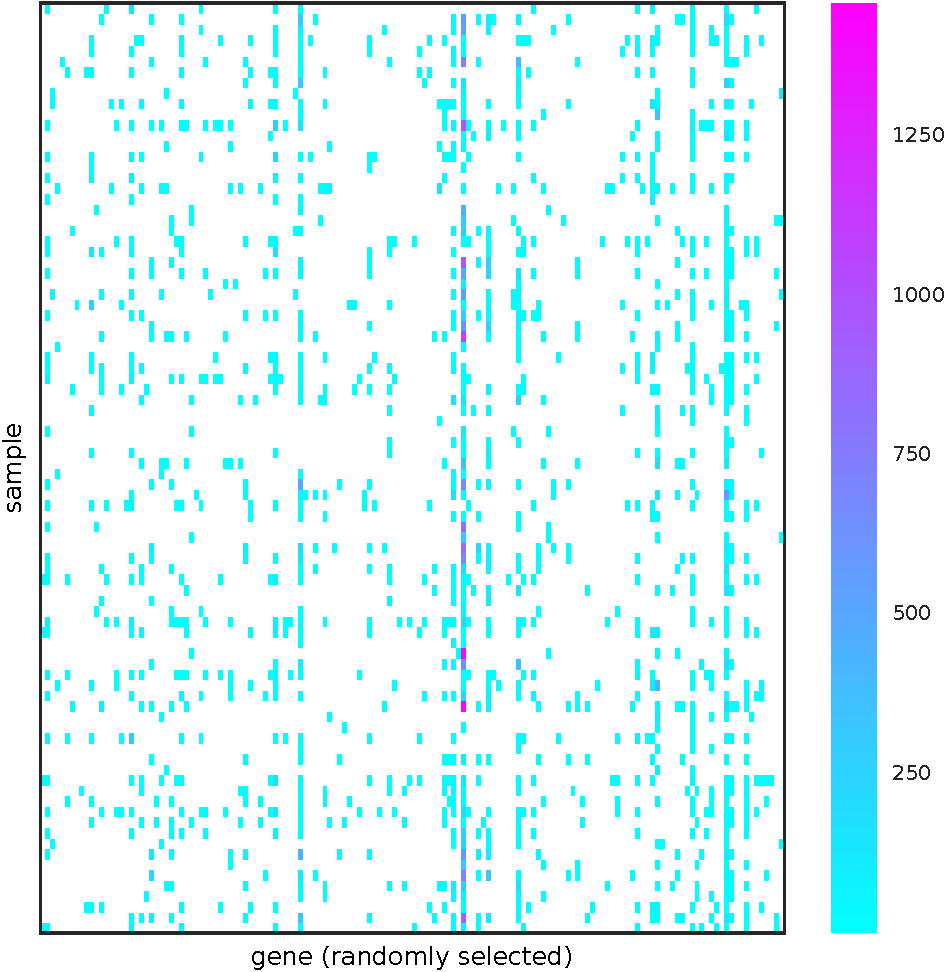
\includegraphics[width=0.8\textwidth]{./tex/chapter3/figures/20170403_sparsity_illustration--754836_nonzero_features.pdf}
    \begin{singlespace}
    \caption[Illustration of the sparsity of the RNA-seq count data]{
        Illustration of the sparsity of the RNA-seq count data.
        Nearly 90\% of measurements of reads per gene per sample are zero, even after removing genes zero reads mapped across samples.
        }
    \label{fig:sparse_RNA-seq}
    \end{singlespace}
\end{figure}


\subsection{General Steps}

%Though preparations for machine learning vary significantly
There are many types of machine learning approaches in the literature.
There are, however, three nearly universal steps for common to all: data normalization/standardization, choice of strategy to limit model complexity, and cross validation.
Each is described below.

\subsubsection{Standardization}
First, standardization of the data is almost always done.
Poor fits are often obtained when features/measurements are on different scales (e.g. inches and miles).
Even if measurements are in comparable units, many algorithms perform better when the features are scaled such that the variances are on a similar scale.
This chapter always scaled the features so each gene had variance = 1, but found centering of features (shift so the mean = 0) to be harmful (see Section \ref{sect:centering_sparse}).

\subsubsection{Model Class Selection \& Limiting Model Complexity}
Next, an appropriate model class needs to be selected.
As discussed above, consideration of $N$ and $d$ have large influence on model selection.
With $N$ = 88 and $d$ = 0.7 million, extra care to limit model complexity is essential.
Fancy algorithms with many parameters (e.g. neural networks) are inappropriate; models that can be limited to a small number of parameters were sought instead.
The two most common penalties for limiting model complexity are L1 (a.k.a. "lasso") \cite{tibshirani1996} (absolute values of coefficients are penalized) and L2 \cite{hoerl1970} (squared coefficients are penalized).
Both limit the coefficient sizes, but L1 leads to more truly zero coefficients \cite{tibshirani1996} and is thus particularly appealing in the $d >> N$ regime, or when some features are expected to be uninformative.
L1 penalties are used by algorithms in several of the methods explored herein.

\subsubsection{Cross Validation} %Evaluate fairly
As emphasized previously, the greatest danger of machine learning is production of a model that will not generalize to future un-seen data.
This can occur because of poorly selected model hyperparameters.
The best practice approach for choosing hyperparameters is cross-validation, whereby the models are trained multiple times, each time with a different portion of the data set aside as a validation set.
The held-out validation set is used to assess the performance of the model trained on the the remaining fraction of the data.
Such cross-validation provides the best framework for tuning parameters without touching the test data, thus reducing over-fitting.

\section{Methods explored}
Machine Learning encompasses broad sets of tools that can be as simple as linear regression or as potentially complex as neural networks.
This chapter uses canonical correlation analysis, a classical statistical tool, and various methods of obtaining and exploring graphs based on the gene-expression partial correlation matrix.

\subsection{CCA}
%Intro
Canonical correlation analysis (CCA) is a classic method dating back to 1936 \cite{hotelling1936} that highlights relationships between two sets of variables \cite{sherry2005}.
In particular, CCA identifies linear combinations of variables that maximize the correlations \footnote{Pearson r, thus "Canonical Correlation" \cite{sherry2005}} between measurements in two matrices.
It can be used as a statistical learning algorithm when the vectors produced predict gene expression of new data that have not been used to fit or assess the model.
In this chapter, if reasonable prediction at the cross-validation step is seen, the genes included in those vectors could highlight interesting biology to target with subsequent experiments.
The utility of CCA was explored by testing for correlation between a linear combination of a set of methylotroph genes and a linear combination of a set of methanotroph genes.
The data used were the tabulated RNA-seq reads after alignment to the 55 isolate genomes, allowing for labeling of species category.
% TODO: Cartoon of vectors.
% TODO (?) Similar to PCA.  PCA explains variance, CCA explains correlation

%Sparsity
The large number of features ($d$) relative to the number of samples ($N$) motivated use of a variation that produces sparse vectors.
In other words, a method was sought that could use regularization to pick out a handful of genes (features) in each category, rather than all features.
The R package PMA\footnote{\url{https://cran.r-project.org/web/packages/PMA/PMA.pdf}} \cite{witten2009} was selected.
CCA variants that focused on both sparsity and compositional data were not found.

\subsection{Gene Expression Partial Correlations}

%Intro
The observational studies of Chapter \ref{chapter:B} were not able to answer the pressing question of what drives the changes in community composition and the patterns of organism distribution (see Figures \ref{fig:4dominant_groups}, \ref{fig:dominant_genera}).
What drives the higher abundance of methylotrophs in the high \ce{O2} samples?
What makes some samples more likely to have high abundances of Bacteroidetes or Burkholderiales?
Do certain methylotrophs flourish when certain methanotrophs express particular sets of genes?

The trends of which genes tend to be co-expressed across samples can help answer these questions.
Correlations are not the best measure to infer causality, as they detect independence rather than dependence \cite{schafer2005}.
%Correlation between gene expression levels can hint at causality, but of course correlation does not imply causality.
A better measure is partial correlation, which measures the strength and directionality of a linear relationship between two variables while controlling for the effects of other variables.
Partial correlations are more likely to be linked to causality than correlations, but are also more difficult to estimate when $d > N$ (see below). % (see Section XX) .

The set of partial correlations can be represented as a graph describing how species interact.
Genes can be represented by nodes, and edges can be added for genes with significant partial correlations \cite{borthagaray2014}.
Once a graph is in hand, community structure can be detected by searching for groups of nodes that are highly connected to each other but have fewer connections to nodes outside the group \cite{hero2012}.
Edges that are labeled by organism type and/or taxonomy can be used to find sub-structures including multiple species.

A reduced version of the partial correlation matrix is desired.
For a network of 0.7M genes (7.0E5), there are approximately 0$.7M^2/2$ ($0.7E11$) potential partial correlation values. % really d(d-1)/2
These partial correlations can be represented in a matrix, or equivalently as edges in a graph.
Clearly the majority of edges are not expected to have meaningful partial correlations, so the goal is to identify the handful of edges that that highlight meaningful biology.
Furthermore, in this $d >> N$ regime, the traditional partial correlation matrix is ill-formed \cite{whittaker2009} such that shrinkage \footnote{similar to regularization} is required.
%In addition, estimation of the partial correlation matrix with this high dimensionality leads to mathematical instability.

There are many potential algorithms that can estimate the reduced set of partial correlations and highlight interesting biology in $d >> N$ regimes.
The Strimmer lab has made great advances in this area \cite{schafer2001, schafer2005, opgen2007shrinkage}.
One Strimmer Lab method uses a shrinkage formula (see the R package \texttt{corpcor}\footnote{\url{http://strimmerlab.org/software/corpcor/index.html}}) and analytic approximations that leads to an estimation of the thinned partial correlation matrix from the gene counts matrix.
They use a shrinkage parameter that shrinks the empirical correlations towards the identity matrix, while leaving empirical variances intact.
While promising, their methods have not been applied to larger omics sets.
The Strimmer group's 2005 paper uses 4,289 genes of \textit{E. coli} and 8 RNA-seq samples \cite{schafer2005}.
The 2007 paper used 800 pre-selected \textit{Aradopsis thaliana} genes \cite{opgen2007Aradopsis}.
%  4,289 protein coding genes of E. coli 8, 15, 22, 45, 68, 90, 150, and 180 minutes after induction of the recombinant protein SOD http://strimmerlab.org/publications/journals/shrinkcov2005.pdf
%In fact, many of their demos are not even demonstrated on the whole set of a single organisms' genes (cite).
This chapter explores the potential of using their methods on larger and higher-sparsity metatranscriptomics data.

Ledoit-Wolf is another route to that uses an empirical rule (no need for cross-validation) to estimate the inverse correlation matrix \cite{ledoit2003}.
This inverse correlation matrix is proportional but not equal to partial correlations.
Further thinning of the network with something such as false discovery rate corrections can be used to thin edges \cite{opgen2007Aradopsis}.

Graphical lasso is another promising method of producing the desired partial correlation network \cite{friedman2008}.
This technique uses L1 regularization to directly compute a sparse matrix of partial correlations.
Cross-validation can be used to optimize the regularization strength.

\subsubsection{Mining the Partial Correlation Matrix}
Even a sparse partial correlation matrix requires computational tools to investigate.
If the top 5\% of potential partial correlation values are kept, this is still $0.05*(1.4E11) = 7.0E9$ edges.
The graphs can be explored by a variety of methods, including NetworkX\footnote{\url{https://networkx.github.io/}} (Python) \cite{schult2008}, and the specialized graph database Neo4j\footnote{\url{https://neo4j.com/}}.

\subsection{Taxonomy of Genes and Contigs}
Knowledge of the taxonomy of genes and contigs are necessary for finding interesting cross-species interactions.
For CCA, taxonomy labels allow separation by microbe type (e.g. methanotrophs vs methylotrophs).
Labels of species in gene-expression partial correlation graphs allow identification of cross-species edges and sub-graphs that include genes from multiple species.
These taxonomic labels can be done at contig level, or the gene level.
Ideally labels at both levels are consistent.

Several methods for obtaining taxonomic labels were explored.
Most tools that assign taxonomic labels (e.g. MEGAN \cite{huson2015}, Kaiju \cite{menzel2016}, Taxator-tk \cite{droge2014}, MetaPhlAn \cite{segata2012}) are designed for individual raw sequencing reads rather than contigs.
Caution must be used when extending these methods to contigs, due to the larger length of contigs and the variable sizes.
For example, taxonomy calls may be made on short, say 100bp regions, of 100kb contigs.
If that region is representative of the whole contig, than a short match works great.
However, aggregating information about matches along the length of the contig should be more robust.

There are few tools designed for contig taxonomy assignments available.
MyTaxa aims to classify contigs using an extension of the Average Amino Acid Identity (AAI) concept \cite{konstantinidis2005}.
This tool was also tested, but appears to be broken and shows no signs of recent maintenance.
Currently a tool for per-gene taxonomic classifications using BLAST best hits and large word sizes is being developed by David Beck.
Additional tools will be required to infer taxonomy across whole contigs, as the labels for genes within a contig will not always agree.


% ================================
% ===== MATERIALS/METHODS ========
% ================================
\section{Materials and Methods}

The data used are RNA-seq counts described in Chapter \ref{chapter:B}.

\subsection{Taxonomy Predictions}
Kaiju \cite{menzel2016} was tested for the ability to predict contig taxonomy.
The settings used included \texttt{-a greedy -e 10000 -x}: greedy mode with up to 10,00 mismatches and filtering of query sequences containing low-complexity regions.
As discussed below (Section \ref{results:taxonomy}), concern about predictions of the taxonomy of long contigs using small portions of their coding sequence led to exploration of BLAST-based methods.
MEGAN was downloaded but was not pursued due to poor support for the command line interface.

\subsection{Canonical Correlation Analysis (CCA)}
CCA was applied to the mappings of the metatranscriptomes of Chapter \ref{chapter:B} to the 55 isolate genomes, in units of RPKM.
Expression levels across genes with the same gene name were pooled.
These data were then split into two matrices: one contained all genes from methanotrophic species and the other contained genes from the non-methanotrophic methylotrophic species.
Gene products having zero variance were removed.

%Features appearing in less than XX of samples were removed.
Each feature was normalized by scaling the variance to 1 with Python's StandardScaler\footnote{\url{http://scikit-learn.org/stable/modules/generated/sklearn.preprocessing.StandardScaler.html}}, but was not centered to have zero mean due to sparsity concerns.
Cross-validation was done to assess predictive accuracy across regularization strengths.
Penalties for the two matrices were kept at the same value, rather than use of a grid search.  %?? Did I ever grid search?  Appears not
% vl = [0.1, 0.2, 0.3, 0.4, 0.5, 0.6, 0.7, 0.8, 0.9]
% [(v, v) for v in vl]
R code was called from Python through rpy2\footnote{\url{https://rpy2.readthedocs.io/en/version_2.8.x/index.html}} \cite{gautier2008}.
All code is available on GitHub: \href{https://github.com/JanetMatsen/CCA_Omics}{CCA\_Omics}.
% TODO: sum on gene product by name.   Reduce number of features.

\subsection{Estimating the Partial Correlation Matrix}

\subsubsection{Prepping Data: Trimming and Normalization}
Data was trimmed and normalized before partial correlation calculations were performed.
First, genes with zero reads assigned across all samples were removed, bringing down the number of features from ~0.9 million to ~0.75 million genes. % 921435 --> 754836
Next, variants of these data with different total numbers of features were prepared by varying a cutoff that accounted for sequencing depth.
The criteria for inclusion was contribution of a specified fraction of reads in at least one sample.
This measure allowed features that were important in one sample, regardless of sequencing depth, to be included.
Dividing by the fraction of reads mapped to coding sequences seemed reckless given low fractions of reads mapped to coding sequences (see Figure \ref{fig:rna_mapping_bars}).
These datasets of varying size were used to test how well various algorithms to scale to this large dataset.

Three approaches were used to approximate the partial correlation matrix: (1) Ledoit-Wolf estimation \cite{ledoit2003}, followed by removing small-magnitude edges, (2) Graphical Lasso \cite{friedman2008} with varying regularization strengths, and (3) the GeneNet \footnote{\url{http://strimmerlab.org/software/genenet/}} package \cite{schafer2001, schafer2005}.
For all three approaches, the variance of each feature was scaled to 1 prior to training the models.
All three were tested on large-memory (244 Gb) AWS instances.

\subsubsection{Ledoit-Wolf}
Estimates of the pseudo-inverse matrix, a matrix proportional to the partial correlation matrix, was estimated via the Python implementation of Ledoit-Wolf\footnote{\url{http://scikit-learn.org/stable/modules/generated/sklearn.covariance.LedoitWolf.html}}.
Data sets of increasing size (increasing number of genes) were tried on an EC2 \texttt{r4.8xlarge} (244GB memory) instance.
The fact that values produced are proportional but not equal to partial correlations prevented use of edge-thinning via false discovery rate tools such as fdrtool\footnote{\url{https://cran.r-project.org/web/packages/fdrtool/fdrtool.pdf}}, which only accept test statistics.
Instead, the partial correlations with the largest magnitude were extracted.
Specifically, the 2.5\% of edges with the most positive, and 2.5\% of the edges with the most negative values were retained.

\subsubsection{Graphical Lasso}
Graphical Lasso was also tested, again with increasing file sizes.
The Scikit-Learn implementation\footnote{\url{http://scikit-learn.org/stable/modules/generated/sklearn.covariance.GraphLasso.html}} \cite{scikit-learn} (Python) was tested, as well as the Huge\footnote{\url{https://cran.r-project.org/web/packages/huge/huge.pdf}} \cite{zhao2012}  package of R, which promises better scalability for large data.

\subsubsection{GeneNet Package}
GeneNet\footnote{\url{https://cran.r-project.org/web/packages/GeneNet/GeneNet.pdf}} was called from R.
This package uses an analytic shrinkage estimator of the correlation matrix, so cross-validation was not required.
%Ran in R (see \href{https://github.com/BeckResearchLab/meta4/blob/master/rnaseq/pcor_new/GeneNet/run_GeneNet_and_summarize.R}{R script}).
Again, genes were trimmed out of the input data if they contributed less than a specified percent in all 88 samples.
The top million edges were explored.

\subsection{Exploring Networks}
%Intro
Different tools were used to explore the resulting matrix structures, in graph form.
Regardless of the software used, the general graph structure included nodes as genes, and edges as partial correlations.
%Nodes were also labeled with taxonomy.

\subsubsection{NetworkX}
Tabular data with one row per edge were loaded into Pandas.
Unique loci were identified, then loaded into NetworkX.
Edges were added by iterating over edge dataframes.
NetworkX haas built-in methods for computing basic network properties such as average connectedness.
See Python code \url{https://github.com/BeckResearchLab/meta4/blob/master/rnaseq/pcor_new/networkx/networkx_helpers.py}.

\subsubsection{Neo4j}
Use of Neo4j was also explored (see \url{https://github.com/JanetMatsen/Neo4j_meta4}).
This database-specific program has a particularly powerful query language, but is slow to develop in without Java programming skills.
A Python API is available, but is more limited than the Java API.


% =================================
% ===== RESULTS/DISCUSSION ========
% =================================
\section{Results and Discussion}

\subsection{Taxonomy Predictions}
\label{results:taxonomy}
Taxonomy calls at the gene and contig level were sought to enable applications of statistical learning that probe interactions between microbes.
While Kaiju produced usable taxonomy calls for the majority of contigs, exploration of these data raised concerns about extrapolation of taxonomic assignments from small match regions to long contigs. %to small regions of the contig to the length of contigs up to XX kb.  %  XX percent of contigs
Currently David Beck is developing a tool for BLAST-based taxonomic assignments of individual genes.
These assignments will be rolled up into contig-level taxonomic predictions.
The statistical learning technique results described below could not use contig taxonomy predictions, but future directions that use this rich layer of information are proposed.

\subsection{Avoid Centering Sparse Data Prior to Learning}
\label{sect:centering_sparse}
Early work for this chapter highlighted the importance of not centering scaled features during preprocessing (Figure \ref{fig:standard_scaler}).
The sparsity of metagenomic data leads to peaks at zero being shifted away from zero during centering. % is not amenable to centering, or the zero peak can is shifted.
The heavier the tail, the greater the shift. %more this peak is shifted away from zero.
These shifted peaks led to strange artifacts in modeling, so centering during preprocessing was always avoided.

\begin{figure}[H]
\centering
    % Originals: /Users/janet/repos/CCA_Omics/code/demo_notebooks/results_for_thesis/170324_example_centered.svg
    % Merged: /Users/janet/Dropbox/thesis/inkscape/170324_standard_scalar.svg.2017_03_24_07_44_42.0.svg
    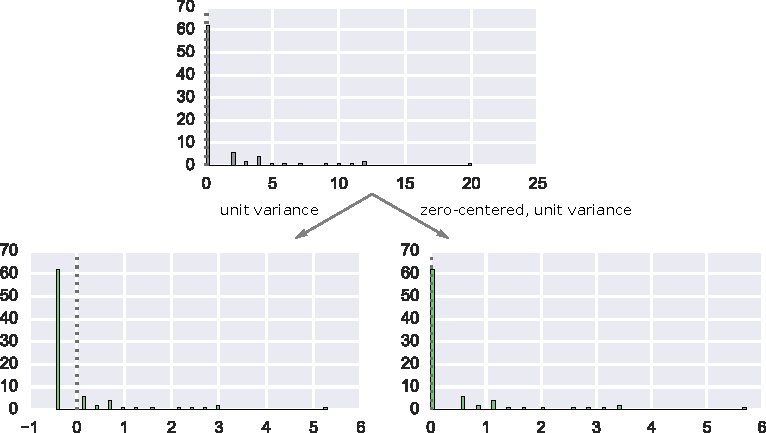
\includegraphics[width=0.8\textwidth]{./tex/chapter3/figures/170324_standard_scalar.pdf}
    \begin{singlespace}
    \caption[Feature scaling: centering sparse features is not advised]{
        When preparing features for machine learning, centering sparse data is not advised.
        All plots have read counts (RPKM, with or without scaling) on the x-axis and the number of samples on the y-axis.
        The top plot shows the untransformed distribution of RPKM for a particular copy of a gene encoding
            "methane monooxygenase component A alpha chain".
        The gene is not expressed in many of the samples, giving the large peak at zero.
        Below, two different normalization schemes are shown:
            standardization so the variance is 1 (left), and
            standardization so the mean is zero and the variance is 1 (right).
        Most machine learning algorithms will produce models with problem artifacts when fitting to such shifted-zero peaks.
        }
    \label{fig:standard_scaler}
    \end{singlespace}
\end{figure}

The CCA results were particularly problematic when features were centered.
Specifically, very high correlations were predicted, but only using features where most measurements had been zero prior to centering.
Variants of CCA that are designed to produce sparse results from sparse data were searched for, but not found.

\subsection{Partial Correlation Matrix Estimation}

\subsubsection{Graphical Lasso}
None of the methods for estimating the partial correlation matrix scaled well to the entire 0.75 million gene dataset.
% TODO: try GeneNet on the whole 0.7M feature data.
The general strategy for exploring algorithm scalability was to run each pipeline on input datasets of increasing size.
The Scikit-learn implementation of Graphical lasso scaled particularly poorly, struggling even with the top 815 features.
It produced floating point errors. % \texttt{FloatingPointError}s:
\texttt{FloatingPointError: Non SPD result: the system is too ill-conditioned for this solver.} % The system is too ill-conditioned for this solver}
In addition the necessity to tune the regularization strength via cross-validation added substantial compute requirements.
Further exploration of this tool is not suggested, unless a few dozen genes have been pre-selected for exploration, as was done in the Strimmer Lab papers.

%\subsubsection{Huge}
The Huge package's variant of graphical lasso scaled better to larger data than the Scikit-learn graphical lasso implementation, but still could not solve large networks.
Instead, other techniques were pursued.

\subsubsection{Ledoit-Wolf}
The Scikit-learn Ledoit-Wolf algorithm scaled reasonably: it was able to approximate the partial correlation matrix for the top 26,968 genes.
The values it reports, however are inverse covariance matrix values, not the partial correlation matrix.
The inverse covariance matrix values are proportional to the partial correlations, but they are not true partial correlations.

Furthermore, genes that are expected to have positive partial correlations in fact had negative values.
To verify this trend, a minimal example was prepared.
The values of 9 genes corresponding to three \textit{pmoCAB} clusters were used, and again the expected within-operon precision matrix values were negative (Figure \ref{fig:pcor_pmocab}).
This may be the result of an unexpected sign convention that is not described in the Python documentation.
Further reading of the Whittaker textbook \cite{whittaker2009} could elucidate the steps needed to get from inverse covariance estimates to partial correlations, and clarify this sign issue.

\begin{figure}[H]
\centering
    % /Users/janet/Dropbox/thesis/tex/chapter3/figures/170403_pMMO_pcor_heatmap.pdf
    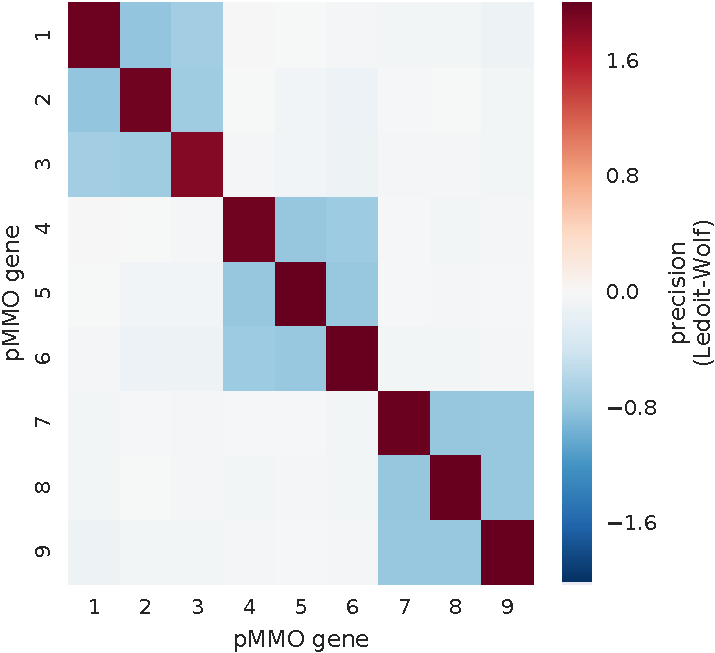
\includegraphics[width=0.7\textwidth]{./tex/chapter3/figures/17045_LedoitWolf_results_on_9_pmo_genes--uncentered.pdf}
    \begin{singlespace}
    \caption[Partial correlation demo: three \textit{pmoCAB} clusters]{
        %The matrix inverse of the covariance matrix, often called the precision matrix, is proportional to the partial correlation matrix
        Ledoit-Wolf estimated precision matrix values (proportional to partial correlations) for a minimal example of 9 genes in three different three-gene \textit{pmoCAB} clusters.
        The read counts were scaled to unit-variance prior to application of the Ledoit-Wolf function in Python's scikit-learn.
        %Notably, the partial correlations for all within-cluster pMMO subunits are negative.
        }
    \label{fig:pcor_pmocab}
    \end{singlespace}
\end{figure}


\subsubsection{GeneNet}
GeneNet provided excellent estimates of the partial correlation matrix.
The algorithms scaled well, despite previous publications having focused on tens or hundreds of genes.

Sequential genes in clusters proved to have the expected positive-valued partial correlations, and an input file of the top 26,968 genes produced partial correlation estimates in about 6 hours on an AWS \texttt{r4.8xlarge} instance (244GB memory). %31,767
Larger networks produced memory errors.
%Larger networks were not tried, as the lowest expressed features are less likely to produce interesting biological stories.

\subsubsection{Validation of the GeneNet Partial Correlation Graph}

Partial correlation graphs were explored with NetworkX and Neo4j.
NetworkX has the large advantage of being quick to program for Python developers, but Neo4j has a much more powerful query language.
The Neo4j query language allows such queries as
%\texttt{MATCH (n)<- [e \{cross_species:'True'\}] -> (m) WHERE n.gene\_product =~'.*transport.*' AND e.pcor\_abs > 0.045 RETURN n, m}
\begin{verbatim}
MATCH (n)<- [e {cross_species:'True'}] -> (m)
    WHERE n.gene_product =~ '.*transport.*'
        AND e.pcor_abs > 0.02
    RETURN n, m
\end{verbatim}
This query demonstrates restriction to cross-species edges where the first gene product of the first node contains the substring``transport" and the partial correlation magnitude is above 0.02.
Neo4j may be used more in future analysis, but the short-term goals of probing the basic network structure were better done using NetworkX.
% gene product of the

%Basics
The top 1 million partial correlation values (edges) had the following distribution (Figure \ref{fig:pcor_hist}):
\begin{figure}[H]
\centering
   % /Users/janet/Documents/Lidstrom Lab Work/meta4_bins_data_and_files/170412_explore_specific_network_as_done_previously/170412_explore_cutoff_0.01/pcor_hist--1e+06_edges.pdf
    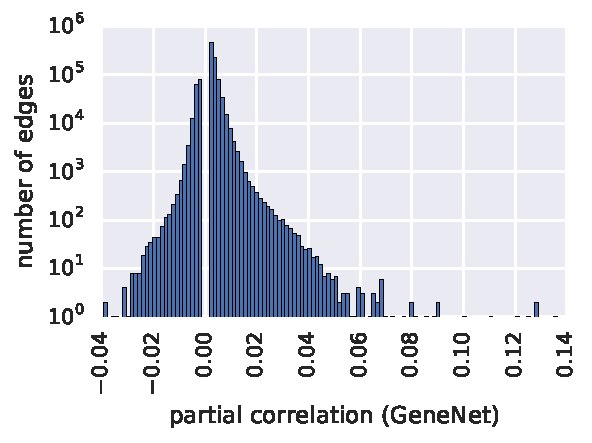
\includegraphics[width=0.6\textwidth]{./tex/chapter3/figures/pcor_hist--1e+06_edges.pdf}
    \begin{singlespace}
    \caption[Distribution of the 1 million partial correlation values with the largest magnitudes]{
        Distribution of the 1 million partial correlation values with the largest magnitudes.
        }
    \label{fig:pcor_hist}
    \end{singlespace}
\end{figure}
This set of one million edges corresponds to 19,850 nodes (genes).
The average degree (edges per node) is 100.8, with the distribution shown in Figure \ref{fig:degree_rank}.
\begin{figure}[H]
\centering
    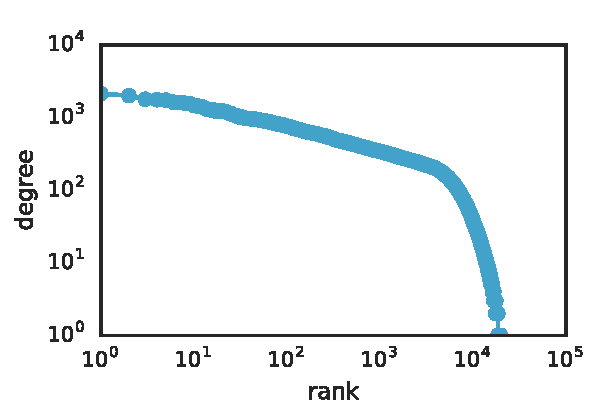
\includegraphics[width=0.6\textwidth]{./tex/chapter3/figures/170406_degree_rank_plot--GeneNet_1e+06_edges--title_deleted_inkscape.pdf}
    \begin{singlespace}
    % /Users/janet/Documents/Lidstrom Lab Work/meta4_bins_data_and_files/170406_GeneNet_on_the_largest_ledoit_Wolf_friendly_file--large_instance/170406_degree_rank_plot--GeneNet_1e+06_edges.svg
    \caption[Degree rank of plot for nodes in GeneNet derived partial correlation network]{
    	Degree rank of plot for nodes in GeneNet derived partial correlation network.
	The most connected nodes are shown on the left, and are each connected to more than 1,000 other genes.
	The least connected nodes have less than 10 connections.
        }
    \label{fig:degree_rank}
    \end{singlespace}
\end{figure}

Initial measures of the validity of the partial correlation matrix focused on the distribution of partial correlations for different sets of genes.
For example, the partial correlations of genes on the same contig are expected to be higher than partial correlations of genes on different contigs.
This turned out to be true (Figure \ref{fig:pcor_same_and_cross_contigs}).

\begin{figure}[H]
\centering
    % /Users/janet/Documents/Lidstrom Lab Work/meta4_bins_data_and_files/170412_explore_specific_network_as_done_previously/170412_explore_cutoff_0.01/same-contig_and_cross-contig_pcor_distributions.pdf
    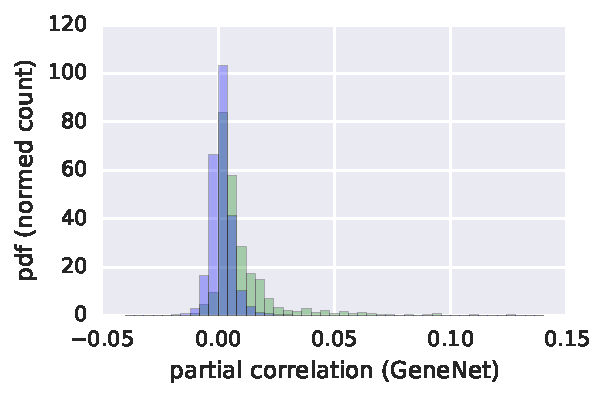
\includegraphics[width=0.6\textwidth]{./tex/chapter3/figures/same-contig_and_cross-contig_pcor_distributions.pdf}
    \begin{singlespace}
    % OLD: /Users/janet/Documents/Lidstrom Lab Work/meta4_bins_data_and_files/170406_GeneNet_on_the_largest_ledoit_Wolf_friendly_file--large_instance/170407_same-contig_and_cross-contig_pcor_distributions.pdf
    \caption[Distribution of partial correlations: same-contig versus across-contig gene pairs]{
    	Distribution of partial correlations: same-contig versus across-contig gene pairs, with each distribution normalized to have unit area.
	    Cross-contig gene pairs (blue bars, 997,276 edges) have lower partial correlations than pairs of genes found on the same contig (green bars, 2,724 edges).
        }
    \label{fig:pcor_same_and_cross_contigs}
    \end{singlespace}
\end{figure}

Similarly, higher partial correlations are expected between subunits of the same protein, or enzymes that are under the same regulation.
This hypothesis was tested by looking at the distribution of partial correlations between subunits of particulate methane monooxygenase \textit{pmo}.
All edges connecting pairs of \textit{pmo} genes were gathered and split into to sets: edges corresponding to the same \textit{pmo} cluster (sequential gene annotations on the same contig), and edges corresponding to two \textit{pmo} genes that are on different contigs or are not sequential.
The distributions (Figure \ref{fig:pmo_pcors}) confirm that subunits of the same operon have higher partial correlation values, adding validity to the GeneNet model.
The same is true for methanol dehydrogenase (\textit{mdh}) subunit pairs (Figure \ref{fig:mdh_pcors}) and hexulose-6-phosphate synthase:hexulose-6-phosphate isomerase gene pairs (Figure \ref{fig:hps_hpi_pcors}).

\begin{figure}[H]
\centering
    % /Users/janet/Documents/Lidstrom Lab Work/meta4_bins_data_and_files/170412_explore_specific_network_as_done_previously/170412_explore_cutoff_0.01/pmo_subunit_pairs_have_higher_pcor--GeneNet--1e+06_edges--horizontal.pdf
    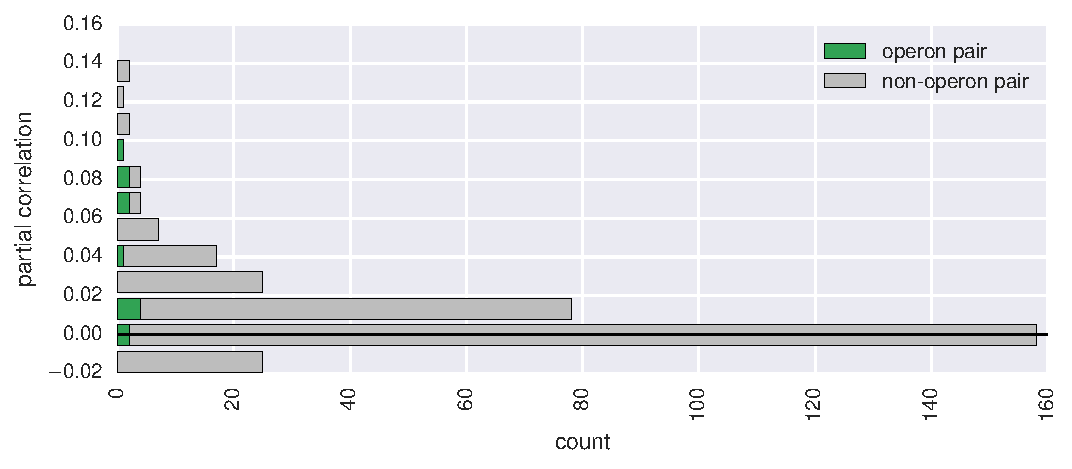
\includegraphics[width=1.0\textwidth]{./tex/chapter3/figures/pmo_subunit_pairs_have_higher_pcor--GeneNet--1e+06_edges--horizontal.pdf}
    \begin{singlespace}
    \caption[Partial correlation values for \textit{pmo}:\textit{pmo} subunit pairs]{
    	Partial correlation values for \textit{pmo}:\textit{pmo} subunit pairs in the GeneNet network.
	Green bars represent pairs that appear to be on the same operon, and gray bars represent all other pairs.
        }
    \label{fig:pmo_pcors}
    \end{singlespace}
\end{figure}

\begin{figure}[H]
\centering
    % /Users/janet/Documents/Lidstrom Lab Work/meta4_bins_data_and_files/170412_explore_specific_network_as_done_previously/170412_explore_cutoff_0.01/mdh-mdh_sequential_pairs--GeneNet--1e+06_genes--horizontal.pdf
    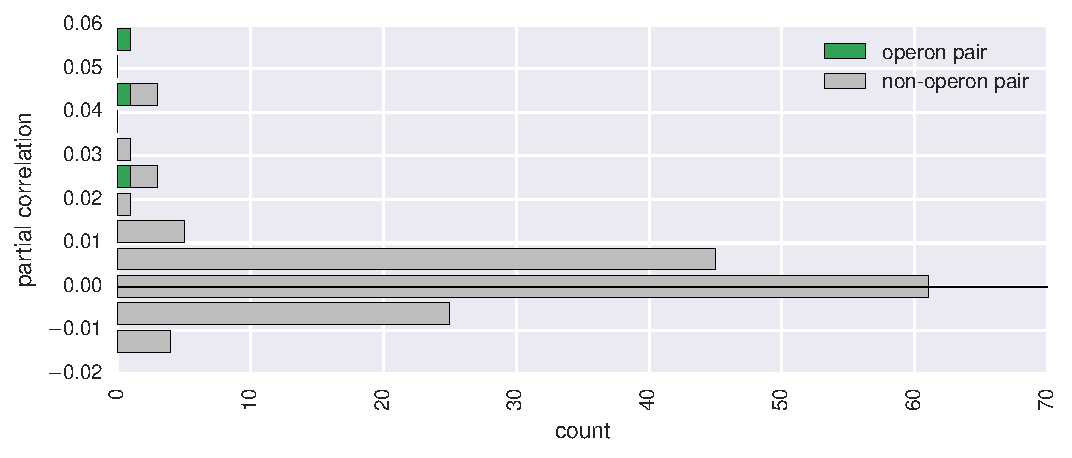
\includegraphics[width=1.0\textwidth]{./tex/chapter3/figures/mdh-mdh_sequential_pairs--GeneNet--1e+06_genes--horizontal.pdf}
    \begin{singlespace}
    \caption[Partial correlation values for \textit{mdh} subunit pairs]{
    	Partial correlation values for \textit{mdh} subunit pairs in the GeneNet network.
	    Green bars represent pairs that are sequential on a contig, and gray bars represent all other pairs.
        }
        \label{fig:mdh_pcors}
    \end{singlespace}
\end{figure}



\subsubsection{Future Directions for GeneNet Analysis}

This chapter identified great potential to use GeneNet for estimation of between-gene partial correlation values.
%There are many next steps for this early stage project.
%First, switching to measuring gene abundance in TPM could be considered, as a means to control for gene length.
%The current iteration used percent of reads in the \texttt{.fastq}, which shed light into how rare the included genes were in these samples, but give smaller %weights to  as the measure of expression for each gene.
%Switching to TPM (Transcripts Per Kilobase Million) could be used instead,
The next step is to mine these graphs for interesting biology.
Community structure can be detected by searching for groups of nodes that are highly connected to each other, but have fewer connections to nodes outside the group \cite{girvan2002}.
Layering in taxonomic labels for nodes will allow the ability to look at partial correlation values between species.

%It should also be possible to detect community structure using social network analysis algorithms.
%A variety are available, though algorithms that can account for edge weights can take advantage of the estimates of partial correlations.


%--------------------------- CCA RESULTS -------------------------------
\subsection{CCA}

CCA was run to see if subsets of genes expressed by methanotrophs have expression that is correlated with subsets of non-methanotrophic methylotroph genes.
The regularization path leading to the optimal objective function had penalties for both vectors equal to 0.026, indicating high regularization.
The vectors it selected for the methanotrophy and methylotrophy genes each included 5 genes, but a correlation of only 0.656.
The genes predicted did not point toward meaningful biology, either (Tables \ref{table:CCA_methanotroph}, \ref{table:CCA_methylotroph}).
This promising technique did not overcome the noise in these RNA-seq data.
Looking back to Figure \ref{fig:isolate_RNAseq}, these null results are likely due to low input data quality.
This method should be revisited when higher-confidence tabulated RNA-seq data becomes available, or used to target other questions.

\begin{table}[H]
\centering
\begin{singlespace}
\caption[Canonical correlation analysis: top features]{Canonical correlation analysis: top methanotroph features.}
\begin{tabular}{l | c | c}
 %\toprule
          gene number & gene name & coefficient  \\
\midrule
	1 & PEP-CTERM protein-sorting domain-containing  protein & 0.977  \\
	2 & heavy metal efflux pump, CzcA family &  0.053  \\
	3 & methionyl-tRNA synthetase &  0.028 \\
	4 & type I restriction enzyme M protein &  0.203 \\
	5 & zinc and cadmium transporter &  0.017 \\
%\bottomrule
\end{tabular}
\label{table:CCA_methanotroph}
\end{singlespace}
\end{table}

\begin{table}[H]
\centering
\begin{singlespace}
\caption[Canonical correlation analysis: top features]{Canonical correlation analysis: top methylotroph features.}
\begin{tabular}{l | c | c}
 %\toprule
          gene number & gene name & coefficient  \\
\midrule
	1 & 3-oxoacyl-[acyl-carrier protein] reductase & 0.214 \\
	2 & GMP synthase (glutamine-hydrolysing) & 0.735 \\
	3 & chaperonin GroEL & 0.544 \\
	4 & citrate synthase & 0.014 \\
	5 & phosphoglucosamine mutase & 0.341 \\
%\bottomrule
\end{tabular}
\label{table:CCA_methylotroph}
\end{singlespace}
\end{table}

% ==========================
% ===== CONCLUSIONS ========
% ==========================
\section{Conclusions}

This chapter described guidelines for applying statistical learning to metatranscriptomics datasets.
It warns against the common practice of centering features in data preprocessing.
Opportunities to use CCA and partial correlation graphs were highlighted.
Given the small $N$ and large $d$ characteristic of metatranscriptomics data, these models are recommended for hypothesis generation rather than predictive modeling.

Two promising software tools were demonstrated for explorations of partial correlation graphs: NetworkX and Neo4j.
NetworkX is powerful and easy to use for Python programmers.  It also has a lot of algorithms built in.
Neo4j has a more user friendly query language, but external packages are usually used when exploration algorithms are needed.

Applications of these techniques will be stronger after refining the tabulated RNA-seq data as is described in Chapter \ref{chapter:B}.



\printendnotes

%
% ==========   Bibliography
%
\nocite{*}   % include everything in the uwthesis.bib file
\bibliographystyle{plain}
\bibliography{uwthesis}
%
% ==========   Appendices
%
\appendix
\raggedbottom\sloppy

% ========== Appendix A

\chapter{Test Appendix}
Appendix, yes, appendix.

\end{document}
